\documentclass[a4paper, 11pt]{memoir}
\author{Gisbert Jan\ss en}
\usepackage{marvosym}
\usepackage{amsfonts}
\usepackage{amssymb}
\usepackage{amsmath}
\usepackage{amsthm}
\usepackage{dcolumn}
\usepackage{bm,bbm}
\usepackage{kpfonts}
\usepackage{braket}
\usepackage{color}
\usepackage{authblk}
\usepackage{graphicx}
\newcommand{\cA}{{\mathcal A}}
\newcommand{\cB}{{\mathcal B}}
\newcommand{\cC}{{\mathcal C}}
\newcommand{\cD}{{\mathcal D}}
\newcommand{\cE}{{\mathcal E}}
\newcommand{\cF}{{\mathcal F}}
\newcommand{\cG}{{\mathcal G}}
\newcommand{\cH}{{\mathcal H}}
\newcommand{\cI}{{\mathcal I}}
\newcommand{\cJ}{{\mathcal J}}
\newcommand{\cK}{{\mathcal K}}
\newcommand{\cL}{{\mathcal L}}
\newcommand{\cM}{{\mathcal M}}
\newcommand{\cN}{{\mathcal N}}
\newcommand{\cO}{{\mathcal O}}
\newcommand{\cP}{{\mathcal P}}
\newcommand{\cQ}{{\mathcal Q}}
\newcommand{\cR}{{\mathcal R}}
\newcommand{\cS}{{\mathcal S}}
\newcommand{\cT}{{\mathcal T}}
\newcommand{\cU}{{\mathcal U}}
\newcommand{\cV}{{\mathcal V}}
\newcommand{\cW}{{\mathcal W}}
\newcommand{\cX}{{\mathcal X}}
\newcommand{\cY}{{\mathcal Y}}
\newcommand{\cZ}{{\mathcal Z}}
\newcommand{\cq}{{\mathcal {CQ}}}

% MATHFRAK LETTERS

\newcommand{\fA}{{\mathfrak A}}
\newcommand{\fB}{{\mathfrak B}}
\newcommand{\fC}{{\mathfrak C}}
\newcommand{\fD}{{\mathfrak D}}
\newcommand{\fE}{{\mathfrak E}}
\newcommand{\fF}{{\mathfrak F}}
\newcommand{\fG}{{\mathfrak G}}
\newcommand{\fH}{{\mathfrak H}}
\newcommand{\fI}{{\mathfrak I}}
\newcommand{\fJ}{{\mathfrak J}}
\newcommand{\fK}{{\mathfrak K}}
\newcommand{\fL}{{\mathfrak L}}
\newcommand{\fM}{{\mathfrak M}}
\newcommand{\fN}{{\mathfrak N}}
\newcommand{\fO}{{\mathfrak O}}
\newcommand{\fP}{{\mathfrak P}}
\newcommand{\fQ}{{\mathfrak Q}}
\newcommand{\fR}{{\mathfrak R}}
\newcommand{\fS}{{\mathfrak S}}
\newcommand{\fT}{{\mathfrak T}}
\newcommand{\fU}{{\mathfrak U}}
\newcommand{\fV}{{\mathfrak V}}
\newcommand{\fW}{{\mathfrak W}}
\newcommand{\fX}{{\mathfrak X}}
\newcommand{\fY}{{\mathfrak Y}}
\newcommand{\fZ}{{\mathfrak Z}}

% MATHBB LETTERS

\newcommand{\bbmC}{{\mathbbm C}}
\newcommand{\bbmE}{{\mathbbm E}}
\newcommand{\bbmN}{{\mathbbm N}}
\newcommand{\bbmH}{{\mathbbm H}}
\newcommand{\bbmM}{{\mathbbm M}}
\newcommand{\bbmR}{{\mathbbm R}}
\newcommand{\bbmQ}{{\mathbbm Q}}
\newcommand{\bbmZ}{{\mathbbm Z}}
\newcommand{\bbmeins}{{\mathbbm 1}}

% MATHBF LETTERS
\newcommand{\spann}{\mathrm{span}}
\newcommand{\expe}{\mathbbm E}
\newcommand{\prob}{\mathrm{Pr}}
\newcommand{\id}{\mathrm{id}}
\newcommand{\V}{\mathcal V}
\newcommand{\tr}{\mathrm{tr}}
\newcommand{\supp}{\mathrm{supp}}
\newcommand{\pot}{\mathrm{Pot}}
\newcommand{\cl}{\mathrm{cl}}
\newcommand{\sr}{\mathrm{sr}}
\newcommand{\bS}{\mathbf S}
\newcommand{\conv}{\mathrm{conv}}
\newcommand{\pr}{\mathfrak{P}}
\newcommand{\rank}{\mathrm{rank}}
\newcommand{\rebd}{\mathrm{rebd}}
\newcommand{\ri}{\mathrm{ri}}
\newcommand{\spec}{\mathrm{spec}}
\newcommand{\aff}{\mathrm{aff}}
\newcommand{\diam}{\mathrm{diam}}
\newcommand{\argmin}{\mathrm{argmin}}
\newcommand{\sign}{\mathrm{sign}}



\newcommand{\bolds}{{\mathbf{s}}}
\newcommand{\boldm}{{\mathbf{m}}}
\newcommand{\boldr}{{\mathbf{r}}}
\newcommand{\bolde}{{\mathbf{e}}}
\newcommand{\boldg}{{\mathbf{g}}}
\newcommand{\boldv}{{\mathbf{v}}}
\newcommand{\boldK}{{\mathbf{K}}}
\newcommand{\boldL}{{\mathbf{L}}}
\newcommand{\boldR}{{\mathbf{R}}}
\newcommand{\boldk}{{\mathbf{k}}}

\newcommand{\bfU}{{\mathbf{U}}}
\newcommand{\bfu}{{\mathbf{u}}}
\newcommand{\bfl}{{\mathbf{l}}}

\newtheorem{theorem}{Theorem}
\newtheorem{acknowledgement}[theorem]{Acknowledgement}
\newtheorem{axiom}[theorem]{Axiom}
%\newtheorem{case}[theorem]{Case}
\newtheorem{claim}[theorem]{Claim}
\newtheorem{conclusion}[theorem]{Conclusion}
\newtheorem{condition}[theorem]{Condition}
\newtheorem{conjecture}[theorem]{Conjecture}
\newtheorem{corollary}[theorem]{Corollary}
\newtheorem{criterion}[theorem]{Criterion}
\newtheorem{convention}[theorem]{Convention}
\newtheorem{definition}[theorem]{Definition}
\newtheorem{example}[theorem]{Example}
\newtheorem{observation}[theorem]{Observation}
\newtheorem{exercise}[theorem]{Exercise}
\newtheorem{lemma}[theorem]{Lemma}
\newtheorem{notation}[theorem]{Notation}
\newtheorem{problem}[theorem]{Problem}
\newtheorem{proposition}[theorem]{Proposition}
\newtheorem{property}[theorem]{Property}
\newtheorem{remark}[theorem]{Remark}
\newtheorem{solution}[theorem]{Solution}
\newtheorem{summary}[theorem]{Summary}
\newcommand{\U}{\mathcal U}
\newcommand{\margpar}[1]{\marginpar{\textcolor{red}{\scriptsize{#1}}}}


\semiisopage
\chapterstyle{komalike}
\usepackage{makeidx}
%\titlehead{Lecture Notes}
\title{Lecture Notes: \\ Quantum Information Theory}
\makeindex
\begin{document}
\maketitle
\tableofcontents

%\part{Basics}


\chapter*{About these notes}
\label{chap:about}
These notes where written as an accompanying document for a quantum information theory master's course held at the ET-IT department at the Munich Technical University, and therefore adresses primarly an audience with classical information theory backround rather than a formal education in quantum mechanics.\\
These notes (as well as the course) intend to provide access to the topic for the uninitiated. Therefore, the focus lies on careful introduction of the underlying structure avoiding to praise the folklore. A downside of this approach is a loss in pace. The contents of the course in consequence only cover a very small fraction of what is nowadays canonical. The motivated reader is referred to the exercises.\\
Especially do these notes not intend to be a textbook on the topic nor should it be regarded as a replacement. The reader is pointed to consult one of the excellent textbooks on the field (we here just mention as examples the books of  Wilde \cite{wilde13}, and Holevo \cite{holevo12a}.) 
Next, we give some overview of the topics of the lectures.  \vspace{3ex} \\
\textbf{Lecture 1.} We introduce the basic entities of quantum theory (for finite-degree systems), and comfort ourselves with its structure by recognizing it as a statistical theory.  \\
\textbf{Lecture 2.} Quantum systems with more than one subsystems are considered. We introduce direct sum and tensor product spaces to describe them. Mathematical tools for describing such systems are introduced. We encounter the first severe "nonclassical" features: Purifications, Entanglement, Noncompatibility. \\
\textbf{Lecture 3.} As a first asymptotical quantum statistical Problem, we discuss the Quantum Hypotheses Testing Problem. We prove a quantum version of Stein's Lemma which acquaints us with the quantum relative entropy.  \\
\textbf{Lecture 4.} Quantum channels, the broades class of allowed transformations of quantum states are introduced as completely positive and trace preserving linear maps. 
We add two important equivalent representation theorems (Kraus decomposition and Stinespring dilation) to our toolbox.  \\
\textbf{Lecture 5.} Source compression of discrete memoryless quantum sources ins considered. The quantum source compression theorem is proved. We get to know the quantum Fidelity, and entanglement fidelity as meaningful figures of merit. The optimal compression rate is determined in terms of the von Neumann entropy. \\
\textbf{Lecture 6.} Transmission of classical messages over disrete and memoryless classical quantum and quantum channels is discussed. The Holevo Theorem is proven to 
determine the classical message transmission capacity. The coding theorem as well as the converse theorem will be derived as implications of Quantum Stein's Lemma. \vspace{3ex}

While it seems, that the quantum Hypotheses testing problem and Quantum Stein's lemma are usually not regarded as part of the canonical arsenal of first-course quantum information theory topics. In this course, Quantum Stein's lemma plays a central role. On one hand, good, capacity achieving classical message transmission codes for quantum channels can be derived from certain good hypothesis tests. On the other hand, Quantum Stein's lemma allows for a elementary "information-theoretic" proof of the monotonicity of quantum relative entropy under quantum channels - which helps to derive most of the important entropy inequalities in quantum information theory. \newline 
The approach to teaching quantum information theory (and teaching it at all) is inspired by I. Bjelakovi\'c and R. Siegmund-Schultze's paper \cite{bjelakovic12a}, which is strongly recommended as additional reference.
















\chapter{Statistical theories in a nutshell}
\label{chap:stat_th}
 In this course, no prior familiarity with quantum theory is assumed. Since our main interest lies in doing information theory for quantum systems, we take a rather short route to get comfortable with the necessary quantum theoretic terminology. \newline 
The approach which best fits our needs, is to regard quantum theory as a mathematical theory to describe the results of a certain type of "statistical" experiments. We already implicitly use such a \emph{statistical theory} ("classical probability theory" ) when considering classical Shannon theory. \newline
The statistical structure of quantum theory arises from the evidence that microscopic objects (e.g. atoms, photons,...) tend to exhibit "random behaviour" in experiments. 
Measurement outcomes fluctuate. However, the following assumption seems to be justified.
\begin{itemize} %\index{statistical axiom}
	\item If a measurement is performed on independent and equally prepared systems in the same condition many times, the relative frequencies 
	\begin{align*}
	f_i := \frac{\text{number of occurencies of the measurement value} \ i}{\text{number of total measurements}}
	\end{align*}
	stabilize (i.e. converge to "probabilities")
\end{itemize}
The above assumption characterizes the hard core of a statistical theory. We will see that there are additional properties a statistical theory should have, and of course there is need to specify, what "measurement", "independent", and "equally prepared"  means. \newline 
It turned out, that the usual "probability theory" used for describing random experiments with coins (and more complex situations) does not suffice
to correctly model some experiments with systems like atoms, photons. \newline 
In the next section, we introduce framework which formulates the specifications of \emph{statistical theory} - in generality sufficient to describe the classical and quantum theories.
\begin{section}{Statistical theories - A general framework}
A real-world statistical experiment is usually divided into two steps
\begin{enumerate}
 \item[(i)] \textbf{Preparation:} Setting a preparation "$P$" to fix the "initial conditions" of the experiment. Examples 
 \begin{itemize}
 \item producing a dice, throwing the dice
 \item filling an urn with a number of balls having each having some letter in $A..Z$, blindly take a ball from the urn
 \item setting up a certain laser configuartion for single photon production
 imprinted.
 \end{itemize} 
  \item[(ii)] \textbf{Registration:} Setting a registration "$R$", i.e. rules how observations are made. Here we assume the most basic type of observation - a "yes/no"-measurement: the registration which one of two given alternatives is taking place. E.g.: 
   \begin{itemize}
   	\item observing if the number showing up on the dice is odd or even
   	\item observing, whether or not the letter $A$ is printed on the ball
   	\item setting up a semipermeable plate in the laser beam and record whether it went through the plate or not.
   \end{itemize}
\end{enumerate}
Usually, in a statistical context, the experiment is performed many times (lets say a large number $N$ of times), the next step is calculating \textbf{relative frequencies}. If $N_i$ is the number of registrations of the $i$th alternative, the relative frequencies are
	\begin{align*}
	f_1 \ = \ \frac{N_1}{N}, \hspace{.3cm}\text{and} \hspace{.5cm} f_2 \ = \ \frac{N_2}{N} = 1 - f_1
	\end{align*}
Having the statistical postulate from the preceding paragraph in mind, we assume, that the relative frequencies stabilize (i.e. converge) in the limit $N \rightarrow \infty$.\newline  
\textbf{Assumption}: There is a number $p(P,R)$ -- the \emph{probability} of registration. 
\newline 
In order to theoretically describe a certain type of experiment, we form equivalence classes,
i.e. we say two preparation procedures $P_1$ and $P_2$ are equivalent, if they lead to the same probabilities for all registration procedures, i.e. $p(P_1,R) = p(P_2, R)$ for all possible $R$. Two registration procedures $R_1, R_2$ are equivalent, if $p(P,R_1) = p(P,R_2)$ for all preparation procedures $P$. We call each equivalence class of preparation procedures a \emph{state}, and each equivalence class of registration procedures an \emph{effect}. 
\begin{enumerate}
	\item [(iv)] \textbf{Theoretical description:} A statistical theory is given by a set $\fS$ of states and a set $\fE$ of effects together with a map $p: \ \fS \times \fE \rightarrow [0,1]$, \ $(s, E) \mapsto p(s,E)$ with
	\begin{align*}
	 p(s_1,E) &= p(s_2,E) \ \text{for all} \ E \in \fE \Rightarrow s_1 = s_2 \\ 
	 p(s,E_1) &= p(s,E_2) \ \text{for all} \ s \in \fS \Rightarrow E_1 = E_2 
	\end{align*}
	we denote the \emph{certain} effect by $\bbmeins$ (i.e. $\bbmeins$ is the unique effect with $p(s, \bbmeins) = 1$ for all states)
\end{enumerate}  
Before we proceed with our exposition of statistical theories, we give the two examples which will be of interest in this course. The first one describes experiments with a "classical system", while the second, regards a "quantum system". 
\begin{example}[Classical statistics]
	Let $\Omega$ be a finite sample set. The statistical theory usually imposed is given by the state set $\fS := \cP(\cX)$, and effect set $\fE := \fE(\Omega)$ with
	\begin{align*}
	  \cP(\Omega) 
		  &:= \left\{ q: \Omega \rightarrow [0,1]: \ \sum_{\omega\in \Omega}q(\omega) = 1 \right\} \\
	  \cE(\Omega)
		  &:= \left\{f: \Omega \rightarrow [0,1]: 0 \leq f(\omega) \leq 1 \ \text{for all} \ \omega \in \Omega   \right\}.
	\end{align*}
	The probability to register the effect $E \in \fE$ when preparing with $q \in \cS$ is
	\begin{align*}
	p(q,E) \ := \ \sum_{\omega \in \Omega} q(\omega) \cdot f(\omega)
	\end{align*}
\end{example}
Note that in the traditional formulation of probability theory after Kolmogorov, rather \emph{events} are considered instead of effects. This approach is recovered by restricting the registration effects to the set
\begin{align*}
\left\{\bbmeins_A: \ A \subset \Omega  \right\} \ \subsetneq \ \fE(\Omega),
\end{align*}
where $\bbmeins_A$ is the indicator function of $A$, i.e. 
\begin{align*}
  \bbmeins_A(\omega) \ := \ 
  \begin{cases}
	  1 	&\text{if} \ \omega \in A \\
	  0  	&\text{otherwise}
  \end{cases}
\end{align*}	
By using the broader concept of effects, we allow also "fuzzy" registrations. 
\begin{example}[Quantum statistics]
Consider a finite-dimensional Hilbert space $\cH = \bbmC^d$, $d < \infty$, the usual statistical model for a quantum system with $d$ degrees of freedom is given by the state set $\fS := \cS(\cH)$, and $\fE := \cE(\cH)$, where 
\begin{align*}
	\cS(\cH) \
	&:= \ \{\rho \in \cL(\cH): \ \rho^\ast = \rho \wedge \rho \geq 0 \wedge \tr\rho = 1\} &\text{(density matrices)}\\
	\cE(\cH) \
	&:= \ \{E \in \cL(\cH): \ 0 \leq E \leq \bbmeins \} 
	&\text{(quantum effects)}
\end{align*} 
 Moreover, for given density matrix $\rho$, and effect $E$, the probability of registration is  calculated via the formula
 \begin{align*}
  p(\rho, E) = \tr \rho E &&\text{(Born's rule)}.
 \end{align*}
\end{example}
 We consider some more aspects of the notions we just introduced.  \newline 
\textbf{Convexity:} When conducting statistical experiments, there usually also is the principal possibility to \emph{mix} preparation procedures as well as registration procedures. For example, when having two preparation devices $P_1, P_2$ at hand, one could let a random number generator decide which one of these to take for the next sample. If $\lambda$ is the probability, that $P_1$ is chosen, it makes sense to demand, that the resulting preparation procedure $\tilde{P}$ is also allowed, and fulfills
 \begin{align}
	p(\tilde{P}, E) = \lambda \cdot p(P_1, R) + (1-\lambda) \cdot p(P_2,R) \label{mixture_of_preparations}
 \end{align} 
 for each registration procedure $R$. Formulating this equation on the level of states and effects, we have
 \begin{align}
    \lambda p(\rho_1, E) + (1-\lambda) p(\rho_2,E) \ 
    &= \lambda \tr \rho_1 E + (1-\lambda) \tr\rho_2 E \\
    &= \tr(\lambda \rho_1 + (1-\lambda)\rho_2)E,
 \end{align}  
 i.e. the state corresponding to a mixture of states $\rho_1, \rho_2$ with mixing parameter $\lambda$ is the corresponding convex combination $\lambda \rho_1 + (1-\lambda) \rho_2$ for each effect $E$. \newline 
 A similar argument can be drawn for mixtures of effects. In consequence, the sets $\cS(\cH)$ and $\cE(\cH)$ are convex subsets of a linear space!
  It is of interests to know the extremal elements of a convex set (i.e. the elements which are not nontrivial convex combinations of other elements of that set). The extremal elements of the set $\fS$ are called \emph{pure states} (accordingly, states which are not pure are called \emph{mixed} \index{mixed state}), while the extremal elements of $\fE$ are called \emph{propositions}. In case of quantum theory, we have
 \begin{proposition}
  Let $\cH$ be (finite dimensional) Hilbert space. The following claims hold. 
  \begin{enumerate}
   \item $\rho \in \cS(\cH)$ is a pure state if and only if it is a rank one projection.
   \item $E \in \cE(\cH)$ is a proposition if and only if it is a projection.
  \end{enumerate} 
 \end{proposition}
  \begin{proof}
  	We show the first claim. The second can be proven by similar arguments. We first show the "$\Rightarrow$" implication. Assume, that $\rho$ is a rank one projection, i.e. it holds
  	%\begin{align}
  	$ \rho^2 = \rho$. 
  	%\end{align}
  	We show, that any convex combination 
  	\begin{align*}
  	\rho = \mu \tau_1 + (1-\mu) \tau_2 \label{thm:density_convexity_2}
  	\end{align*}
  	is necessarily trivial. It holds
  	\begin{align*}
  	\rho - \rho^2  
  	&= \mu \tau_1 + (1-\mu) \tau_2 - \mu^2 \tau_1^2 - \mu(1-\mu) (\tau_1 \tau_2 + \tau_2 \tau_1) - (1-\mu)^2 \tau_2^2 \\
  	&= \mu (\tau_1 - \tau_1^2) + (1- \mu) (\tau_2 - \tau_2^2) + \mu(1-\mu) (\tau_1 - \tau_2)^2 \\
  	&\geq \mu(1-\mu)^2 (\tau_1 - \tau_2)^2 \\
  	&\geq 0.
  	\end{align*}
  	The equalities above are by rearranging terms. The first inequality above (notice: the inequality is a matrix inequality in the hermitian semiorder) is by
  	the fact, that $\mu$ and $1 -\mu$ are nonnegative and $(\tau_1 - \tau_1^2)$ as well as $\tau_2 - \tau_2^2$ are positive semidefinite matrices (check this.) 
  	The second inequality follows, because $(\tau_1 - \tau_2)^2$ is positive semidefinite. Since $\rho - \rho^2 = 0$ ($\rho$ is assumed to be a projections),
  	it holds 
  	\begin{align}
  	\mu (1 - \mu) (\tau_1 - \tau_2)^2 = 0.
  	\end{align}
  	But this is only possible if $\mu \in \{0,1\}$ or $\tau_1 = \tau_2$, which is the case if and only if the convex combination in Eq. (\ref{thm:density_convexity_2})
  	is trivial. \newline 
  	For the showing remaining "$\Leftarrow$" implication, let $\rho$ be an extremal element of $\cS(\cH)$. Consider a spectral decomposition 
  	\begin{align}
  	\rho = \sum_{i=1}^{\dim \cH} \lambda_i \ket{\psi_i}\bra{\psi_i}
  	\end{align}
  	of $\rho$. Notice that this is a convex combination of $\rho$. Since $\rho$ is assumed to be extremal there is exactly one $i_0$ with $\lambda_{i_0} =1$, while $\lambda_i = 0$
  	for all $i \neq i_0$. Consequently
  	$\rho = \ket{\psi_{i_0}}\bra{\psi_{i_0}}$,
  	a rank one projection.
  \end{proof}
  \begin{remark}
  	Each unit vector $v \in \cH$ gives rise to a pure state $\rho = \ket{v}\bra{v}$. 
  	the correspondence $v \leftrightarrow \ket{v}\bra{v}$ is one-to-one up to global phases, i.e. for $\theta \in \bbmR$, $v$ and $e^{i\theta} v$ give rise to the same pure 
  	state. 
  \end{remark}
   To describe statistical experiments with more than two outcomes, we introduce the concept of an observable. An \emph{observable} (or \emph{measurement}) \index{observable} \index{measurement} with a (finite) set $\cY$ of measurement outcomes is a function $F: \cY \rightarrow \fE$ such that 
   \begin{align}
    \sum_{y \in \cY} E_y \ = \ \bbmeins
   \end{align}
	Since the set of measurement values is finite, it is more common to define a measurement by a collection of effects. In case of quantum theory, we define
   \begin{definition}
   	 Let $\cH$ be a finite dimensional Hilbert space, and $\cY$ be a finite set. A POVM (positive operator valued measure) on $\cH$ with measurement outcomes in $\cY$ is a family $\{E_y\}_{y \in \cY}$ such that 
   	 \begin{enumerate}
   	 	\item $0 \leq E_y \leq \bbmeins_\cH$ for all $y \in \cY$
   	 	\item $\sum_{y \in \cY} E_y = \bbmeins_\cH$. 
   	 \end{enumerate}
   	 The special case, of a family of mutually orthogonal projections in $\cH$ is called \emph{projection valued measure (PVM)} or simply \index{projection valued measure}  \emph{von Neumann measurement} \index{measurement!von Neumann}.
   \end{definition}
	In this course we restrict ourselves to finite dimensional Hilbert spaces and finite sets of measurement values, which avoids topological and measure theoretic issues. The interested reader may consult the following references for more details. 
\begin{enumerate}
 \item K. Kraus, \emph{States, Effects and Operations}, Springer, 1983
 \item A. Holevo, \emph{Quantum Systems, Channels, Information}, de Gruyter, 2012, Chapter 2.
 \item A. Holevo, \emph{Probabilistic and Statistical Aspcects of Quantum Theory}, Edizione de Scuola Normale Superiore Pisa, 2011, Chaper 1
 \item S. Gudder, \emph{Stochastic Methods of Quantum Mechanics}, Dover Publications, 2005, Chapter 4
 \end{enumerate}
\end{section}

\begin{section}{Example: Qubit systems} \index{qubit}
  To get into calculations with the mathematical objects defined above, we consider the case of a quantum system with two degrees of freedom, i.e. the underlying Hilbert space is two-dimensional.
  Despite the fact, that such systems are often considered in physics\footnote{Real-world examples of such systems are e.g. the spin of an electron system or the polarization of light.}, they can be 
  regarded as quantum counterparts of classical bit systems bit systems with alphabet $|\cX| = 2$. The set $\cS(\bbmC^2)$ of qubit states has a convenient pictoral representation in $\bbmR^3$, which we derive 
  next. The matrices
  \begin{align*} \index{Pauli matrices}
   \sigma_0 &=  \left(\begin{array}{c c} 1 & 0 \\ 0 & 1 \end{array}\right)  \hspace{.5cm}
   \sigma_1 =  \left(\begin{array}{c c} 0 & 1 \\ 1 & 0 \end{array}\right) \\
   \sigma_2 &=  \left(\begin{array}{c c} 0 & - i \\ i & 0 \end{array}\right) \hspace{.5cm}  
   \sigma_3 =  \left(\begin{array}{c c} 1 & 0 \\ 0 & -1 \end{array}\right)  
  \end{align*}
  are called \emph{Pauli matrices} and form an orthogonal basis in $\cL(\bbmC^2)$, it holds  
  \begin{align}
    \braket{\sigma_i, \sigma_j}_{HS} =  2 \delta_{ij}.
  \end{align}
  If we normalize each of the matrices with a factor $1/\sqrt{2}$ we obtain an orthonormal basis. We can write each matrix $A \in \cL(\cH)$ as a linear combination
  \begin{align}
   A = \frac{1}{2} \sum_{i=0}^3 r_i \sigma_i. \label{bloch_linear_comb} 
  \end{align}
   with $r_i = \braket{A, \sigma_i}_{HS}$. We aim to derive conditions on the numbers $r_0,\dots,r_3$ being equivalent to $A \in \cS(\cH)$. We have
   \begin{enumerate}
    \item Each $r_i$ has to be real, because $A$ is Hermitian. 
    \item $r_0 = 1$ holds because of the property $\tr(A) = 1$. 
    \item Since $A \geq 0$ holds, 
     \begin{align}
      \frac{1}{4}(r_0^2 - r_1^2 - r_2^2 - r_3^2) = \det A \geq 0.
     \end{align}
     Since $r_0 = 1$, we obtain the condition $\|r\| \leq 1$ for the vector $(r_1,r_2,r_3)^T \in \bbmR^3$. 
   \end{enumerate}
   On the other hand, if $A$ is represented as in (\ref{bloch_linear_comb}) with $r_0 = $ and $(r_1,r_2,r_3)^T$ an element of $B_1(0)$, the euclidean ball around $0$ with radius one, then $A \in \cS(\cH)$ is 
   implied. Indeed, $1 = r_0 = \tr A$, and $\det A = 1 - r_1^2 - r_2^2 - r_3^2 \geq 0$. Consequently, $A$ is a density matrix. Since the basis coefficients $r_0,r_1,r_2,r_3$ of an element of $\cL(\cH)$
   are unique, the map which connects each density matrix with its bloch vector $(r_1,r_2,r_3)^T$ is a one-to-one. By linearity of the Hilbert-Schmidt scalar product, it is clear that this map is also 
   affine. Therefore, we have introduced an affine bijection of $\cS(\cH)$ onto the radius one euclidean ball in $\bbmR^3$. By this fact, it is clear, that the set of extremals of $\cS(\cH)$ correspond to
   the set of extremals of $B_1(0)$, i.e. the unit sphere around $0$ in $\bbmR^3$.
   \begin{remark}
    In quantum optics, it is common, to specify the polarization preparation of a leaser beam by giving the corresponding bloch vector $r = (r_1,r_2,r_3)^T$. Examples are (according to www.wikipedia.de)
    \begin{align*} 
    &  \left(\begin{array}{c} 1 \\ 0 \\ 0 \end{array}\right) \hspace{.5cm} \text{(linear horizontal)}  
    & \left(\begin{array}{c} -1 \\ 0 \\ 0 \end{array}\right) \hspace{.5cm} \text{(linear vertical)}   \\
    &  \left(\begin{array}{c} 0 \\ 1 \\ 0 \end{array}\right) \hspace{.5cm} \text{(linear 45}^{\circ}\text{)}  
    & \left(\begin{array}{c} 0\\ -1 \\ 0 \end{array}\right) \hspace{.5cm} \text{(linear -45}^{\circ}\text{)}  \\ 
    &  \left(\begin{array}{c} 0 \\ 0 \\ 1 \end{array}\right) \hspace{.5cm} \text{(right circular)}  
    & \left(\begin{array}{c} 0\\ 0 \\ -1 \end{array}\right) \hspace{.5cm} \text{(left circular)}   \\
    & \left(\begin{array}{c} 0\\ 0 \\ 0 \end{array}\right) \hspace{.5cm} \text{(unpolarized)}.   
    \end{align*}
   \end{remark}
   By calculating their bloch vectors, one can verify, that the pure states $P_i := \ket{e_i}\bra{e_i}$, $i \in \{0,1\}$ are located at the north and south poles of the Bloch ball. The set of states 
   which lie on the straight line connecting the pure states $P_0$ and $P_1$ are parameterized by probability distributions on $\{0,1\}$, 
   \begin{align*}
    \left\{P(p) := p(0) P_0 + p(1) P_1\right\}.
   \end{align*}
   In fact, each straight line connecting two antipodes on the Bloch sphere can be regarded as a version of the classical bit states. 
   %Proceeding with this discussion, we observe an essential difference between
   %the set of bit and the set of qubit states. ???
   
  % \begin{exercise}
  %  Calculate the Bloch vectors of the states $P_{\pm} := \ket{f_\pm} \bra{f_\pm}$ where
  %  \begin{align*}
  %   f_{\pm} := \tfrac{1}{\sqrt{2}}(e_0 \pm e_1).
  %  \end{align*}
  %  Where are their images located on the Bloch ball?
  % \end{exercise}
 %\end{section}

  
  %\begin{section}{Exercises}
   
   %\begin{exercise}
   %	compatibility
   %\end{exercise}
   
   %\begin{exercise} 
   % Prove, that the set of POVMs on a Hilbert space all indexed by the same alphabet form a convex set.
   %\end{exercise}
   
   %\begin{exercise}
   % Consider the set of probability distributions $\cP(\cX)$ on the alphabet $\cX := \{1,2,3\}$ find a useful geometric picture in $\bbmR^3$. 
   %\end{exercise}
   
   %\begin{exercise}
   % Where are the pure qubit states located in the Bloch ball, where the maximally mixed state 
   % \begin{align}
   %  \pi_2 := \left(\begin{array}{cc} 
   %          \tfrac{1}{2} & 0 \\
   %           0 	& \tfrac{1}{2}
   %         \end{array} \right)
   % \end{align}
   %\end{exercise}
   
   %\begin{exercise}
    %Consider the orthonormal basis $\cB := \{f_+, f_-\}$ defined by
    %\begin{align}
    % f_{+} := \tfrac{1}{\sqrt{2}}(e_0 + e_1) \hspace{.3cm} \text{and} \hspace{.3cm} f_{-} := \tfrac{1}{\sqrt{2}}(e_0 - e_1).
   % \end{align}
   % Calculate the Bloch vectors $r_1,r_2,r_3$, and draw them into the Bloch ball picture. 
   %\end{exercise}
   %\begin{exercise}
   	%Show, that two mixtures
   	%\begin{align}
   	% \sum_{i=1}^I \lambda_i \ket{\psi_i}\bra{\psi_i} \hspace{.2cm} \text{and} \hspace{.2cm} \sum_{j=1}^J \mu_i \ket{\phi_j}\bra{\phi_j}
   	%\end{align}
   	%are pure state decompositions of the same density matrix if and only if 
   	%...
   %\end{exercise}

 % \end{section}











\chapter{Composite quantum systems}
\label{chap:comp_sys}
 In the preceding lecture, we introduced the basic quantum-theoretic entities for given quantum system with Hilbert space $\cH$. In this lecture, we consider quantum systems
which are composed of two or more \emph{subsystems}. E.g. we need to be able to describe the statistics of experiments where two electron spins (each with Hilbert space $\cH = \bbmC^2$) are involved. 
It is one of the major tasks in information theory, to quantify correlations between such subsystems and optimally exploit statistical properties of composite systems for usage in communication protocols. \\
Remembering classical statistical theory (with finite sample spaces), the state of a system composed of $n < \infty$ subsystems with alphabets $\cX_1,\dots,\cX_n$ the set of states on that system 
is the set $\cP(\cX_1 \times \cdots \times \cX_n)$ of probability distributions on the cartesian product of $\cX_1,\dots,\cX_n$. We notice, that the pure states are exactly the products of point measures, $\{\delta_{x^n}: \ x^n \in \cX^n \}$ with 
\begin{align*}
 \delta_{x^n}(y^n) := \prod_{i=1}^n \delta_{x_i}(y_i) && (x^n = (x_1,\dots,x_n), y^n = (y_1,\dots,y_n)).
\end{align*} 
Taking as an example $n=2$, we can define to each $p \in \cP(\cX \times \cX_2)$ the \emph{marginal states} $p_1 \in \cP(\cX_1), p_2 \in \cP(\cX_2)$ by
\begin{align*}
p_1(x_1) := \sum_{x_2 \in \cX_2} \ p(x_1,x_2), \hspace{.3cm} \text{and} \hspace{.7cm} p_2(x_2) := \sum_{x_1 \in \cX_1} p(x_1,x_2)  
\end{align*}
which recover the statistical properties of the individual subsystems. The systems are statistically \emph{independent}, if the state $p$ is a product distribution, i.e. with some $p_1 \in \cP(\cX_1), \ p_2 \in \cP(\cX_2)$ it holds
\begin{align*}
   p(A \times B) \ = \ p_1(A)\cdot p_2(B)
\end{align*}
for all $A \subset \cX_1$, $B \subset \cX_2$ (the usual notation is then "$p = p_1 \otimes p_2$".) We notice, that each $w \in \cP(\cX_1 \times \cX_2)$ can be written as a convex combination of product states via
\begin{align*}
 w \ = \ \sum_{x^n \in \cX_1 \times \cdots \times \cX_n} w(x^n)  \ \delta_{x^n}.
\end{align*}
Regarding a composite quantum system with subsystem Hilbert spaces $\cH_1,\dots, \cH_n$, we need to define the states on that Hilbert space. Therefore, the cartesian product $\cH_1 \times \dots \times \cH_N$ has to be equipped with a Hilbert space structure. 
\begin{subsection}{Mathematical Interlude -- Direct sums and tensor products}
 In this course, we will make extensive use of two different possibilites to provide the cartesian product 
 \begin{align*}
  V_1 \times \cdots \times V_N \ := \ \left\{ (v_1,\dots, v_N): \  v_i \in V_i, \ 1 \leq i \leq N \right\}
 \end{align*}
 of linear spaces $V_1,\dots, V_n$ with a linear structure, the \emph{direct sum}\index{linear space!direct sum} $V_1 \oplus \cdots \oplus V_n$ and the \emph{tensor product} $V_1 \otimes \cdots \otimes V_n$\index{linear space!tensor product}. Since we are always dealing with Euclidean
 spaces, we assume $V_i$ to be equipped with a scalar product $\braket{\cdot,\cdot}_i$, $i = 1,\dots, n$. 
 \end{subsection}
 \begin{subsection}{Direct sum spaces}
 The direct sum $V_1 \oplus \cdots \oplus V_N$ of $V_1, \dots, V_N$ is defined as the set
 \begin{align*}
   \left\{ \left(\begin{array}{c} v \\ w   \end{array}\right): \ v \in V_1,\ w \in V_2 \right\}
 \end{align*}
 together with the obvious linear structure inherited from the component spaces by using addition and scalar multiplication component-wise, i.e.
 \begin{align*}
  \lambda \cdot \left(\begin{array}{c} v_1 \\ \vdots \\ v_N   \end{array}\right) \ 
  & =  \ \left(\begin{array}{c} \lambda \cdot  v_1 \\ \vdots \\ \lambda \cdot v_N   \end{array}\right) &(\lambda \in \bbmC, v_1 \in V_i, \ 1 \leq i \leq N), \ \text{and} \\ 
  \left(\begin{array}{c} v_1 \\ \vdots \\ v_N   \end{array}\right) + \left(\begin{array}{c} w_1 \\ \vdots \\ w_N   \end{array}\right) \
  & = \ \left(\begin{array}{c} v_1 + w_1 \\ \vdots \\  v_N + w_N   \end{array}\right) &(v_i, w_i \in V_i, \ 1 \leq i \leq N).
 \end{align*}
 We may also define a scalar product $\braket{\cdot,\cdot}_{1 \oplus \dots \oplus N}: V_1 \cdots \oplus V_N \rightarrow \bbmC$ by setting
 \begin{align*}
  \left\langle \left(\begin{array}{c}v_1 \\ \vdots \\ v_N \end{array}\right), \left(\begin{array}{c}w_1 \\ \vdots \\ w_N \end{array} \right) \right\rangle_{1 \oplus \dots \oplus N} := \sum_{i=1}^N \braket{v_i,w_i}_i 
 \end{align*}
 for all $v_i,w_i \in V_i$, $1 \leq i \leq N$. On the other hand, if $\cH$ is a Hilbert space, and $V_1,\dots, V_N \subset \cH$ are pairwise orthogonal linear subspaces such that for each $h \in \cH$
 exist uniquely $h_1 \in V_1, \dots, \ h_N \in V_N$ such that $h = h_1 + \dots + h_N$, then $\cH$ is isomorphic to $V_1 \oplus \dots \oplus V_N$. We can define injections 
 \begin{align*}
  I_j \in \cL(V_j, \cH), \hspace{.2cm}  v \mapsto I_j (v) = (0, \dots,v, \dots, 0) &&(v \in V_j).
 \end{align*}
 Notice, that the adjoints are given by $I_j^\ast(h) = P_j h$, where $P_j$ is the projector onto $V_j$ for $j \in [N]$. Choosing an appropriate orthonormal basis, each $A \in \cL(\cH)$ can be 
 written as a \emph{block matrix} \index{matrix!block}
 \begin{align*}
  A = \left(\begin{array}{ccc}
  A_{11} & \cdots & A_{1N} \\ 
  \vdots & \ddots& \vdots \\ 
  A_{N1} & \cdots & A_{NN} \end{array}\right) 
 \end{align*}
 where $A_{ij} = I_j^\ast AI_i\in \cL(V_i, V_j)$ is a smaller matrix for all $i,j \in [N]$.
 \begin{exercise}
  Show, that 
  if $\{v_i\}_{i=1}^{\dim V_1}\subset V_1$ and $\{w_j\}_{j=1}^{\dim V_2} \subset V_2$ are orthonormal bases in $V_1$, $V_2$, then
   \begin{align}
    \left\{\left(\begin{array}{c} v_i \\ 0 \end{array} \right) \right\}_{i=1}^{\dim V_1} \ \cup \ \left\{\left(\begin{array}{c} 0 \\ w_i \end{array} \right) \right\}_{j=1}^{\dim V_2}
   \end{align}
   is an orthonormal basis in $V_1 \oplus V_2$ according to the corresponding scalar product. In particular, $\dim V_1 \oplus V_2 = \dim V_1 + \dim V_2$.
 \end{exercise}
 \end{subsection}
 \begin{subsection}{Tensor product spaces}
  Another way to equip the cartesian product of $V_1, \dots, V_N$ with a linear structure is forming the tensor product. First, we note, that each 
  pair $(v_1,\dots, v_N) \in V_1 \times \cdots \times V_N$ defines a $N$-linear function $v_1 \otimes  \otimes v_N: V_1 \times \dots \times V_N \rightarrow \bbmC$ by
  \begin{align*}
   v_1 \otimes \dots \otimes v_N (x_1,\dots, x_N) := \braket{v_1, x_1}_1\cdot \dots \cdot \braket{v_N,x_N}_N. 
  \end{align*}
  The definitions can be obviously extended to form linear combinations of these \emph{elementary tensors}, i.e. the rules
  \begin{align*}
    \lambda (v \otimes w) 
    &= (\lambda v) \otimes w = v \otimes (\lambda w)  &(\lambda \in \bbmC, v \in V_1, w \in V_2) , \\
    (v_1 + v_2) \otimes w 
    &= v_1 \otimes w + v_2 \otimes w &(v_1,v_2 \in V_1, w \in V_2) \\
    v \otimes (w_1 + w_2)
    &= v \otimes w_1 + v \otimes w_2 &(v \in V_1, w_1, w_2 \in V_2) 
  \end{align*}
  apply (the rules above are formulated for $N=2$, but it is quite clear how the version for general finite $N$ looks). We can form formal linear combinations 
  \begin{align*}
   \sum_{i=1}^N \alpha_{i_1\dots i_N} v_{i_1} \otimes \cdots \otimes v_{i_N}
  \end{align*}
  of elementary tensor product vectors with coefficients $\alpha_{i_1\dots i_N} \in \bbmC$. The set 
  \begin{align*}
   V_1 \otimes \cdots \otimes V_N := \spann \{v_1 \otimes \cdots \otimes v_N: \  v_i \in V_i, \ 1 \leq i \leq N\}
  \end{align*}
  is called the tensor product of $V_1$ and $V_2$. We also can extend these structures to the linear maps. With spaces $V_1, \dots, V_N, \tilde{V}_1, \dots  
  \tilde{V}_N$, we define the tensor product $\cL(V_1,\tilde{V}_1) \otimes \dots \otimes \cL(V_N, \tilde{V}_N)$ accordingly. For each $A_1,\dots,A_N$, $A_i \in \cL(V_i,\tilde{V_i})$, $A_1 \otimes \cdots \otimes A_N$ is the map defined by 
  \begin{align*}
   (A \otimes \cdots \otimes A_N)(v_1 \otimes \cdots \otimes v_N) 
   = A_1v_1 \otimes \cdots \otimes A_N v_N
  \end{align*}
  for each $v_1 \in V_1, \dots, v_N \in V_N$. We have
  \begin{align*}
     \cL(V_1 \otimes V_2, \tilde{V}_1 \otimes \tilde{V}_2) 
   &= \ \cL(V_1, \tilde{V}_1) \otimes \cdots \otimes \cL(V_N, \tilde{V}_N)  \\
   &= \ \spann \{A_1 \otimes \cdots A_N: \ A_i \in \cL(V_i, \tilde{V}_i), \ 1 \leq i \leq N\}.
  \end{align*}
  
 \end{subsection}
  \begin{subsection}{Isomorphisms and representations} 
 
 In calculations and proofs, it is sometimes advantageous, to transfer the objects under investigation to another space. In the following we collect some isomorphisms
 which are often used. The definitions below are defined for members of the canonical euclidean orthonormal basis, but extend -- by linearity -- to all elements of the underlying spaces. 
 \begin{enumerate}
  \item 
 \begin{align*}
   \Sigma: \ \bigoplus_{i=1}^N \cH \   
   \rightarrow \ \cH \otimes \bbmC^N,  \hspace{.8cm}
    \left(\begin{array}{c} v_1 \\ \vdots \\ v_N \end{array} \right)  \mapsto \sum_{i=1}^N v_i \otimes e_i 
 \end{align*}
 \item 
 \begin{align}
  \Gamma: \ \cL(\cH_1,\cH_2) \ \rightarrow \ \cH_1 \otimes \cH_2 \hspace{.8cm} \ket{v}\bra{w} \  \mapsto \ \ket{\overline{w}} \otimes \ket{v} \label{def:iso_gamma}
 \end{align}
 \item 
 \begin{align*}
  \Lambda: \ \cL(\bbmC^M \otimes \bbmC^N) \ 
   \rightarrow  \ \cL\left(\bigoplus_{i=1}^M \bbmC^N\right) \ \hspace{.8cm}
   \ket{e_i} \bra{e_j} \otimes \ket{e_k}\bra{e_l} \
   \mapsto  I_i^\ast \ket{e_k}\bra{e_l} I_j
  \end{align*}
 \end{enumerate}
With the preparations, we are able to define quantum states on composite systems.
\begin{definition} 
 The set of states of a composite system with $N < \infty$ subsystems, $\cH_i$ being the Hilbert space of the $i$-th subsystem is given by the set
 \begin{align*}
  \cS\left(\bigotimes_{i=1}^N \ \cH_i \right)
 \end{align*}
 of density matrices on the tensor product $\bigotimes_{i=1}^{N} \ \cH_i := \cH_1 \otimes \dots \otimes \cH_N$ of the spaces $\cH_1, \dots \cH_N$. 
\end{definition}
A corresponding map to form ``marginal states'' on subsystems is given by the partial trace, which we define for notational simplicity for bipartite
systems (i.e. composite systems consisting of two subsystems). 
\begin{definition}[Partial trace] \index{partial trace} \index{trace!partial}
 For two Hilbert spaces $\cH_1, \cH_2$, the partial trace (over $\cH_2$) is the linear map
 \begin{align*}
  \tr_{\cH_2}: \ \cL(\cH_1 \otimes \cH_2) \rightarrow \cL(\cH_1) 
 \end{align*} 
 defined by 
 \begin{align*}
  \tr_{\cH_2}(\ket{u \otimes v}\bra{ w \otimes x}) := \braket{x,v} \ket{u}\bra{w} &&(u,w \in \cH_1, \ v,x \in \cH_2)
 \end{align*}
 plus linear extension. The corresponding partial trace over $\cH_1$, $\tr_{\cH_1}$ is defined analogeously. 
\end{definition}
 We demonstrate by example, how the partial trace can be calculated. Let $\cH_1, \cH_2$ be Hilbert spaces, $\dim \cH_i = d_i$, $i = 1,2$.  
 Let $A \in \cL(\cH_1 \otimes \cH_2)$, with orthonormal tensor basis decomposition
 \begin{align*}
  A = \sum_{i,j=1}^{d_1} \sum_{k,l=1}^{d_2} \ a_{ijkl} \ \ket{f_i \otimes g_k} \bra{f_j \otimes g_l}. 
 \end{align*}
 Then, we calculate
 \begin{align*}
  \tr_{\cH_2}(A) 
  &= \sum_{i,j=1}^{d_1} \sum_{k,l=1}^{d_2} \ a_{ijkl} \ \tr_{\cH_2}(\ket{f_i \otimes g_k} \bra{f_j \otimes g_l}) \\
  &= \sum_{i,j=1}^{d_1} \sum_{k}^{d_2} \ a_{ijkl} \ \braket{f_l, f_k} \cdot \ket{f_i} \bra{f_j} \\
  &= \sum_{i,j=1}^{d_1}  \left(\sum_{k}^{d_2} \ a_{ijkk}\right)  \cdot \ket{f_i} \bra{f_j}.
 \end{align*}
  Note, that the definition of partial traces easily extends to composite systems with more than two subsystems. Let $N$ parties (each of them with Hilbert space 
  $\cK_i$ assigned, share a system with Hilbert space $\cK_1 \otimes \dots \otimes \cK_N$. To apply the partial trace on the $j$-th system one uses the definition
  above with $\cH_1 = \bigotimes_{i \neq j} \cK_i$, $\cH_2 := \cH_i$ and so on...
  \begin{proposition}
  Let $A \in \cL(\cH_1 \otimes \cH_2)$. It holds 
  \begin{enumerate}
   \item $\tr(A) = \tr(\tr_{\cH_1}(A)) = \tr(\tr_{\cH_2}(A))$,
   \item $\tr(\tr_{\cH_2}(A)B) = \tr(A(B \otimes \bbmeins_{\cH_2}))$,
   \item $A \geq 0 \ \Rightarrow \ \tr_{\cH_2}(A) \geq 0$,
   \item $\rho \in \cS(\cH_1 \otimes \cH_2) \ \Rightarrow \ \tr_{\cH_2}(\rho) \in \cS(\cH_2)$. 
  \end{enumerate}
 \end{proposition}
  \begin{proof}
   The claims of the proposition can be verified by straightforward calculation, left as an exercise. As an example, we show the second claim. Let $x \in \cH_1$, $\|x\| =1$. Note, that 
   \begin{align*}
    P:= \ket{x}\bra{x} \otimes \bbmeins_{\cH_2}
   \end{align*}
   is a projection. We have
   \begin{align*}
    \braket{x, \tr_{\cH_2}(A) x}  
    \ =\ \tr(\ket{x}\bra{x} \tr_{\cH_2}(A)) 
    \ =\ \tr(A^{\tfrac{1}{2}}PA^{\tfrac{1}{2}}) 
    \ \geq\  0.
   \end{align*}
  \end{proof}
  Here, we may point out a significant difference between the concept of a bipartite state in classical theory and quantum theory. As noticed earlier, each classical bipartite state (i.e. probability distribution on a product alphabet) 
   can be written as a convex combination of product distributions. Quantum probability 
   offers an additional class of states beyond. 
  \begin{definition} \label{def:bipartite_state_classification}
   A state $\rho \in \cS(\cH_1 \otimes \cH_2)$ is called
   \begin{enumerate}
    \item[(i)] \emph{"uncorrelated", "product state"} \index{quantum state!product}, if it can be written $\rho = \rho_1 \otimes \rho_2$ for some $\rho_1 \in \cS(\cH_1)$, $\rho_2 \in \cS(\cH_2)$. 
    \item[(ii)] \emph{"separable state"} \index{quantum state!separable}, if it admits the form 
    \begin{align*}
     \rho = \sum_{i=1}^N \lambda_i \ \rho_1^{(i)} \otimes \rho_2^{(i)}
    \end{align*}
    with $N \in \bbmN$, $\lambda_i \in (0,1)$, $\rho_1^{(i)} \in \cS(\cH_1)$, and $\rho_2^{(i)} \in \cS(\cH_2)$ for all $i \in [N]$, $\sum_{i=1}^N \lambda_i = 1$. 
    \item[(iii)] \emph{entangled} \index{quantum state!entangled} otherwise.
   \end{enumerate}
  \end{definition}
   \begin{remark}
    One could ask about infinite or even uncountable convex combinations of product states. These are identified as uncorrelated by means of Caratheodory's theorem. 
    It asserts, that for given convex subset $A \subset \bbmR^d$, each element $x \in A$ can be written as a convex combination of at most $d+1$ extremal elements in 
    $A$. Consequently, each separable state can be written as a finite convex combination of not more than $2d+1$ product states. 
   \end{remark}
   A closer look at Definition \ref{def:bipartite_state_classification} reveals, that beyond the convex combinations of product states (of which the product states itself are a trivial
   subclass), there is another class of states having no classical counterpart. The class of entangled states is indeed nonempty, as the following example demonstrates.
	Let two unit vectors $\varphi_1, \varphi_2 \in \bbmC^d$ with $\varphi_1 \perp \varphi_2$, and nonzero coefficients $\alpha, \beta \in \bbmC$, $|\alpha|^2 + |\beta|^2 = 1$ be given. We
	show, that 
	\begin{align}
	\eta  \ = \ \alpha \varphi_1 \otimes \varphi_1 + \beta \varphi_2 \otimes \varphi_2 \label{ex_entangled_state_1}
	\end{align}
    is state vector of an entangled state. In fact, the assumption, that $\eta$ is separable leads to a contradiction. Let $\{\varphi_1,\varphi_2,\dots,\varphi_d\}$ be an extension of $\varphi_1,\varphi_2$ to an orthonormal basis in $\bbmC^d$. Since $\eta$ is pure and separable, it takes the form of a product vector
    \begin{align}
     \eta \ = \ \left(\sum_{i=1}^d c_i \varphi_i \right) \otimes \left(\sum_{i=1}^d \tilde{c}_j \varphi_j\right) \ = \ \sum_{i,j=1}^d c_i \tilde{c}_j \varphi_i \otimes \varphi_j.
     \label{ex_entangled_state_2}
    \end{align}
    Comparing coefficients in (\ref{ex_entangled_state_1}) and (\ref{ex_entangled_state_2}), shows, that 
    \begin{align}
     c_1 \cdot \tilde{c}_1 \ = \alpha, \hspace{.3cm} c_2 \cdot \tilde{c}_2 \ = \beta, \hspace{.3cm} c_i \cdot \tilde{c_j} \ = \ 0 \ \text{for} \  i \neq j \ \text{or} \ i,j > 2.
    \end{align}
    As a consequence of the above equalities, $\alpha \cdot \beta = c_1 \cdot \tilde{c}_2 \cdot \tilde{c}_1 \cdot c_2  = 0$, which is a contradiction to $\alpha, \beta \neq 0$. We record
   \begin{example}
	A pure bipartite state $\eta = \alpha \cdot \varphi_1 \otimes \varphi_1 + \beta \cdot \varphi_2 \otimes \varphi_2$, $|\alpha|^2 + |\beta|^2 = 1$ is entangled if and only if $\alpha, \beta \neq 0$.
   \end{example}

	\end{subsection}
	\begin{subsection}{Schmidt decomposition}
    Especially useful is the following ``polar'' representation of vectors on a tensor product. 
   \begin{theorem}\label{theorem:schmidt_decomposition} \index{decomposition!Schmidt -}
    Let $a \in \cH_1 \otimes \cH_2$. Then there exist ortonormal systems $\{v_i\}_{i=1}^m \subset \cH_1$, $\{w_i\}_{i=1}^m \subset \cH_2$ and numbers 
    $\alpha_1 \geq \alpha_2 \geq \dots \geq \alpha_m > 0$, such that 
    \begin{align*}
     a = \sum_{i=1}^m \sqrt{\alpha_i} v_i \otimes w_i \label{theorem:schmidt_decomposition_1}
    \end{align*}
    holds. 
   \end{theorem}
   \begin{remark}
    \begin{enumerate}
     \item $m$ is usually called the \emph{Schmidt number}\index{Schmidt number} of $a$, $\sqrt{\alpha_1}, \dots, \sqrt{\alpha_m}$ the \emph{Schmidt coefficients}
     \index{Schmidt coefficients}.
     \item It holds 
     \begin{align*}
      A_1 := \tr_{\cH_2}(\ket{a}\bra{a}) &= \sum_{i=1}^{m} \alpha_i \ket{v_i}\bra{v_i} \\
      A_2 := \tr_{\cH_1}(\ket{a}\bra{a}) &= \sum_{i=1}^{m} \alpha_i \ket{w_i}\bra{w_i}. 
     \end{align*}
      In particular the Schmidt coefficients are the nonzero eigenvalues (counted with their multiplicities), and the vectors in the orthonormal systems which appear in 
      the Schmidt decomposition are the corresponding eigenvectors.
    \end{enumerate}
	\end{remark}
    Though formulated for general bipartite vectors, we will use the Schmidt decomposition most of the time for pure quantum states. 
    The Schmidt decomposition Theorem is essentially a reformulation of the singular value decomposition, see Theorem \ref{thm:svd}. 
    \begin{proof}[Proof of Theorem \ref{theorem:schmidt_decomposition}]
	 Using the inverse of the linear isomorphism $\Gamma$ from (\ref{def:iso_gamma}), we
	 obtain a matrix $A = \Gamma^{-1}(\ket{a})$. Let
	 \begin{align*}
	 A = \sum_{i,j=1}^{m} \sqrt{\alpha_i} \ket{v_i}\overline{\bra{w_i}}
	 \end{align*}
	 be a singular value decomposition of $A$. Then 
	 \begin{align*}
	  a \ = \Gamma \circ \Gamma^{-1} a = \sum_{i=1}^m \sqrt{\alpha_i} \ \Gamma(\ket{w_i}\overline{\bra{v_i}}) = \sum_{i=1}^m \sqrt{\alpha_i} v_i \otimes w_i.
	 \end{align*}
    \end{proof}
	As we will see in forthcoming lectures, Schmidt decomposition is a very convenient way to write a pure bipartite state in proofs and calculations. Unfortunately, there seems to be no general satisfactory extension of Theorem \ref{theorem:schmidt_decomposition} to spaces with more than two tensor factors. Nevertheless, Schmidt decompositions allows us to construct "purifications" of states, we define.
	\begin{definition}[Purification] \index{purification}		
	  Let $\rho \in \cS(\cH)$ be a state, and $\cK$ be an additional Hilbert space. The pure state $\ket{\Psi}\bra{\Psi}$ is a \emph{purification} of $\rho$ if, $\tr_\cK \ket{\Psi}\bra{\Psi} = \rho$. 
	\end{definition}
	The Schmidt decomposition offers a nice principle to construct purifications of a state $\rho$. By the remark following Theorem \ref{theorem:schmidt_decomposition}, the Schmidt coefficients and the orthonormal vectors in one tensor factor in Schmidt decompositions are obtained from a spectral decomposition of $\rho$. The remaining Schmidt vectors can be chosen freely on any Hilbert space of sufficient dimension (see Exercise \ref{ex:schmidt_dec}). 
		\begin{observation} \label{obs:mon_ent}
		A quantum system in a pure state can only be uncorrelated to the ``outside world'', i.e. if $\rho \in \cS(\cH \otimes \cK)$ is such that $\tr_\cK \rho$ is pure, it is necessarily a product state.
	\end{observation}
	The above observation also holds in for the classical statistical theory. However, in quantum information theory, this insight becomes a powerful tool when combined with the possiblity to "purify" quantum systems. The bipartite pure state resulting from purification captures all correlations of the system "to the outside world". This is a "quantum feature", since purifying systems is not possible in classical theory (see Exercise \ref{ex:class_pur}.)
	\end{subsection}
     \begin{section}{Supplement: Entanglement witnesses}
      \begin{definition}[Entanglement witness]
      A matrix $A \in \cL^h(\cH_A \otimes \cH_B)$ is called an \emph{entanglement witness} \index{entanglement!witness}, if it is not positive semidefinite, and 
      \begin{align}
       \tr A(\rho \otimes \sigma) \geq 0 
      \end{align}
      for all $\rho \in \cS(\cH_A)$, $\sigma \in \cS(\cH_B)$. An entangled state $\tau$ is said to be \emph{detected} by $A$, if 
      \begin{align}
       \tr A \tau < 0.
      \end{align}
     \end{definition}

     \begin{definition}
      A hyperplane in $\bbmR^m$ is a set of the form
      \begin{align}
       H(\xi, k) := \{z \in \bbmR^m: \braket{\xi,z} = k\},
      \end{align}
      where $\xi \in \bbmR^m \setminus \{0\}$, and $k \in \bbmR$. $H(\xi,k)$ is said to separate two sets $S_1, S_2 \subset \bbmR^m$, if 
     \end{definition}
     Some properties 
     \begin{enumerate}
      \item $H(\xi,k) \perp span \{\xi\}$
      \item $\forall x,y \in H(\xi,k) ,\lambda \in \bbmR$, it holds $\braket{\lambda, \xi, x -y}$
     \end{enumerate}
     
     
     \begin{theorem}[Separating Hyperplanes] \label{thm:separating_hyperplanes}
     If $S$ is a closed convex subset of $\bbmR^m$, and $x_0 \notin S$, then there exists a hyperplane separating $x_0$ and $S$.
     \end{theorem}
  
     \begin{proof}
      First step. We show, that there is a unique $s_0 \in S$ minimizing the distance $|s-x_0|$. Such an $s_0$ exists, because $S$ is closed. Namely, choosing a sequence $\{s_i\}_{i \in \bbmN}$ such that 
      \begin{align}
       \underset{k \rightarrow \infty}{\lim}|s_k - x_0| = \underset{s \in S}{\inf}|s - x_0|
      \end{align}
      holds. By the Bolzano-Weierstrass Theorem (``Every bounded sequence has a convergent subsequence''), we find a subsequence $\{s_{k(j)}\}_{j=1}^\infty$, which converges to an $s_0 \in \bbmR^m$, which is 
      also a member of $S$, since by hypothesis, $S$ is closed. Consequently,
      \begin{align}
       |s_0 - x_0| \ = \ \underset{j \rightarrow \infty}{\lim} |s_{k(j)} - x_0| \ = \ \underset{k \rightarrow \infty}{\lim} |s_k - x_0| \ = \ \underset{s \in S}{\inf} |s -x_0|.
      \end{align}
      We show uniqueness by contradiction. Assume that another element $s' \in S$ also fulfills the mentioned condition, i.e.   
      \begin{align}
       |s' - x_0|  \ = \ \underset{s \in S}{\inf} |s' - x_0|. 
      \end{align}
      Then $|s' - x_0| = |s_0 - x_0|$, and $x_0, s_0, s'$ form an isosceles triangle. But then the midpoint of $\overline{s_0s')}$ (which is by convexity of $S$ also a member of $S$), is closer to $x_0$ than $s_0$, a 
      contradiction! \\
      As a second step, we construct a hyperplane which separates $s_0$ and $x_0$. We set
      \begin{align}
       \xi := x_0 - s_0, \ \text{and} \hspace{.5cm} \hat{\xi} := s_0 + \tfrac{1}{2} \xi.
      \end{align}
      We have
      \begin{align}
       k \ := \ \braket{\xi,\hat{\xi}} \ = \ \braket{x_0 - s_0, \tfrac{1}{2}(x_0 + s_0)} \ = \ \tfrac{1}{2}(|x_0|^2 - |s_0|^2).
      \end{align}
      By construction, $H(\xi, k)$, the hyperplane perpendicular to $\xi$, going through $\hat{\xi}$, fulfills
      \begin{align}
       0 \ < \ \tfrac{1}{2} |s_0 - x_0|^2 = \frac{1}{2}(\braket{\xi,s_0} - \braket{\xi,x_0})
      \end{align}
      Therefore, $H(\xi, k)$ is a separating Hyperplane for $s_0$ and $x_0$, since
      \begin{align}
       \braket{\xi, x_0} \ < \frac{1}{2}(\braket{\xi,s_0} - \braket{\xi,x_0}) \ < \ \braket{\xi, s_0}.
      \end{align}
      In the last two steps of the proof, we convince ourselves, that $H(\xi, k)$ is indeed separating $x_0$ and $S$. \\
      Step three. We show $H(\xi,k) \cap S = \emptyset$. Assume that $s_1 \in H(\xi,k) \cap S$, i.e. $\braket{\xi,s_1} = k$. Consider the isosceles triangle with vertices $s_1,x_0,s_0$. Let $s_2$ be a point on
      $\overline{s_0s_1}$ for which $\overline{xs_2} \perp \overline{s_0s_1}$. Then 
      \begin{align}
       |x_0 - s_2| \ < \ |x_0-s_0|,
      \end{align}
      which is a contradiction, because $s_2 \in S$. consequently the constructed hyperplane and $S$ do not intersect. \\
      Fourth step. We show, again by contradiction, that $\braket{\xi, s} > k$ for all $s \in S$, i.e. $H(\xi, k)$ separates $S$ from $x_0$. Assume hat $s_1 \in S$ and $\alpha_1 := \braket{\xi,s_1} \leq k$. 
      We already know from Step 2, that $\alpha_0 := \braket{\xi,s_0} > k$. Define
      \begin{align}
       \lambda \ := \ \frac{k - \alpha_1}{\alpha_0 - \alpha_1}.
      \end{align}
      Notice, that $\lambda$ is in $[0,1)$, since
      \begin{align}
       \alpha_0 \ > \ k \ \geq \alpha_1.
      \end{align}
      By convexity of $S$, 
      \begin{align}
       s_2 := \lambda s_0 + (1-\lambda) s_1 \  \in \ S,
      \end{align}
      which is a contradiction, because
     \begin{align}
      \braket{\xi,s_2} = \lambda \alpha_0 + (1-\lambda) \alpha_1 = k.
     \end{align}      
     \end{proof}
     Although we formulated the separating hyperplane Theorem for $\bbmR^m$ and euclidean scalar product $\braket{\cdot,\cdot}$, there is no obstacle in using it for the set $\cL(\cH)$ equipped with the Hilbert scalar 
     product $\braket{\cdot,\cdot}_{HS}$ on that space. Indeed $\Gamma: \ \bbmR^{2m^2} \ \rightarrow \ \cL(\cH)$ with
     \begin{align}
      A \ \mapsto (\Re(a_{11}),\dots, \Re(a_{mm}),\Im(a_{11}), \dots, \Im(a_{mm}))
     \end{align}
     sets up a linear isomorphism between $\bbmR^{2m^2}$ and $\cL(\cH)$, and it is easily checked, that
     \begin{align}
      \braket{A,B}_{HS} \ = \ \braket{\Gamma(A), \Gamma(B)} 
     \end{align}
     for all $A,B \in \cL(\cH)$. 
     \begin{theorem}
      A state $\rho \in \cS(\cH_A \otimes \cH_B)$ is
     \begin{itemize}
      \item separable, if and only if $\tr\rho A \geq 0$ for each entanglement witness $A$. 
      \item entangled, if and only if there exists an entanglement witness $A$, such that $\tr \rho A < 0$.
     \end{itemize}
     \end{theorem}
     \begin{proof}
      The both claims of the above theorem are easily seen to be equivalent. We prove the first claim. Asssume, that $\rho$ is separable. By defnition, $\tr \rho A \geq 0$ for each entanglement 
      witness $A$. for the converse statement, we notice, that the set of separable states on $\cS(\cH_A \otimes \cH_B)$ is a closed convex subset of $\cL(\cH)$. By Theorem \ref{thm:separating_hyperplanes} and
      the remark after its proof, we find a Hyperplane $H(A,k) \subset \cL(\cH)$, such that $\braket{A,\sigma}_{HS} \geq k$ for each member $\sigma$ of the separable density matrix, and $\braket{A,\rho} < k$.
      Consequently, $A - k \bbmeins_{\cH_A \otimes \cH_B}$ is an entanglement witness for $\rho$.
     \end{proof}
    \end{section}
   \begin{section}{Exercises}
     \begin{exercise}[Non-cyclicity of the partial trace]
     	Find an example of matrices $A,B \in \cL(\cH_1 \otimes \cH_2)$ such that 
     	$\tr_{\cH_2}(AB) \ \neq \ \tr_{\cH_2}(BA)$ holds.
     \end{exercise}
     
   \begin{exercise}[Compatibility problems]
   Let $q \in \cP(\cX_1 \times \cX_2)$, $r \in \cP(\cX_2 \times \cX_3)$ be probability distributions. They are called \emph{compatible}, if there is a probability distribution $p \in \cP(\cX_1 \times \cX_2 \times \cX_3)$ 
   having $q$ and $r$ as marginals on $\cX_1 \times \cX_2$ and $\cX_2 \times \cX_3$ respectively. 
   \begin{itemize}
    \item Show, that $q, r$ are compatible if and only if their marginals on the ``shared alphabet'' $\cX_2$ coincide.
    \item Show, by counterexample, that an analogue of the above equivalence does not hold for density matrices. (Hint: Monogamy of entanglement).
   \end{itemize}
   \end{exercise}
   \begin{exercise}
    Mixing may cause destruction of entanglement. Convince yourself by straightforward calculation, that the equidistributed mixture 
    \begin{align}
     \rho := \frac{1}{2}(\ket{\Phi_+}\bra{\Phi_+} + \ket{\Phi_-}\bra{\Phi_-})
    \end{align}
   of the so-called singlet states with state vectors $\Phi_+$ and $\Phi_-$,
   \begin{align}
    \Phi_{\pm} := \frac{1}{\sqrt{2}}( e_0 \otimes e_0 \pm e_1 \otimes e_1 ) 
   \end{align}
   is in fact separable.
   \end{exercise}
   \begin{exercise}
    The set of separable density matrices in $\cS(\cH_A \otimes \cH_B)$ is convex by definition. What are the extremal elements?
   \end{exercise}
	\begin{exercise}\label{ex:schmidt_dec}
		Let $\rho \in \cS(\cH)$ be a quantum state. What is the minimum dimension of a Hilbert space $\cK$ such that we find a purification of $\rho$ on $\cS(\cH \otimes \cK)$?
    \end{exercise}
    \begin{exercise}
	  Let $\rho \in \cS(\cH)$ be a density matrix with spectral decomposition $\sum_{i=1}^r \lambda_i \ket{f_i}\bra{f_i}$. Show, that with a pure maximally entangled state $\Phi := \ket{\phi}\bra{\phi}$ with state vector
	  \begin{align*}
	   \phi \ := \ \frac{1}{\sqrt{r}} \sum_{i=1}^{r} f_i \otimes f_i
	  \end{align*} 
	  on $\cH \otimes \cH$, 
	  \begin{align*}
		 \psi := (\bbmeins_{\cH} \otimes \rho^{\frac{1}{2}})\phi 
	  \end{align*}
	  is state vector of a purification of $\rho$.
    \end{exercise}
	\begin{exercise}[Classical purifications] \label{ex:class_pur}
	Let $p \in \cP(\cX)$ be mixed. There exists no $\cY$ such that $r \in \cP(\cX \times \cY)$ is pure and the $\cX$-marginal is $p$.
	\end{exercise}
  %   \margpar{Include \begin{itemize}
  %   		\item Exercises on Block matrices
  %   		\item Positivy preservation under isomorphisms
   %  		\item GHZ state
  %   	\end{itemize}}
   \end{section}
   
    

 
 
 
  
 
 
   



\chapter{Quantum hypotheses testing - Quantum Stein's Lemma}
\label{chap:hypotheses_tests}
 In this lecture we consider the "asymmetric quantum hypothesis testing" problem. Assume, an experimenter is confronted with a source which emits pairwise independent and equally prepared quantum systems. Given two a priori density matrices  
$\sigma_0$ (called ``null hypothesis''), or $\sigma_1$ (called ``alternative hypothesis'') the goal is to decide by measurements on the outputs, which preparation is present. 
We prove ``Quantum  Stein's lemma'', 
which quantifies the behaviour of the error of optimal tests for this task in a situation, where large numbers of outputs of the systems are available for 
performing tests. \\
This lecture is central to the course for two reasons. A first one is, that hypothesis tests also make up for good  message transmission codes. This fact is already known
from classical Shannon information theory. However, this relation seems to be even more important for quantum systems, as we will see in subsequent sections. A second reason
is, that Stein's lemma allows a very simple and illuminating proof of the \emph{monotonicity of the quantum relative entropy under completely positive and trace preserving maps}, 
which is notoriously hard to prove otherwise. After all, this will be our entrance to several highly notrivial quantum entropic inequalities which are essential for proving 
major results in quantum Shannon theory. \\
The mentioned strategy to prove entropy inequalities starting from Quantum Stein's lemma is strongly inspired by the paper \cite{bjelakovic12a}, where also the relatively elementary proof 
of the result given below can be found. The interested reader also should consult that work. 
To formally settle the above described situation, assume, we are confronted with a preparation device which emits quantum systems pairwise uncorellated and 
additionally all being prepared according to the same density matrix. If this density matrix is $\gamma$, the mentioned properties of the preparation device ensure us, that 
the statistical behaviour of the joint quantum state of $n$ systems (``\emph{blocklength} $n$'') prepared is described by the density matrix 
\begin{align*}
\gamma^{\otimes n} := \underbrace{\gamma \otimes \cdots \otimes \gamma}_{n \ \text{times}}
\end{align*}
To settle the (asymetric) Hypothesis test problem, assume now, that the state $\gamma$ is unknown to the receiver of the systems. The receiver is provided with two 
a priori hypotheses in form of density matrices $\rho$ (``null hypothesis'') and $\sigma$ (``alternative hypothesis''), and tries by measurement on the outputs,
to decide, which of these hypothesis to accept. For a given test $\{E_0,E_1\}$ on the $n$-fold output system, two kinds of errors can happen 
\begin{enumerate}
	\item \textbf{First kind error:} The actual density matrix is $\rho$, but $\sigma$ is detected. This happens with probability 
	\begin{align*}
	\tr E_1 \rho^{\otimes n} = \tr (\bbmeins - E_0) \rho^{\otimes n}
	\end{align*}
	\item \textbf{Second kind error:} The density matrix is $\sigma$, but $\rho$ is detected. This happens with probability 
	\begin{align*}
	\tr E_0 \sigma^{\otimes n}
	\end{align*}
\end{enumerate}
\section{Quantum Stein's Lemma}
A common goal now is, to determine the optimal asymptotical behaviour of the second kind error for tests whose first kind error is below a threshold $\epsilon \in (0,1)$. 
For this reason, we define for each $\epsilon \in [0,1]$
\begin{align*}
 \beta_{\epsilon,n}(\rho, \sigma) := \inf\left\{\tr(a \sigma^{\otimes n}): 
 \ 0 \leq a \leq \bbmeins_\cH^{\otimes n} \ \text{and} \ \tr(a \rho^{\otimes n}) \geq 1 - \epsilon \right\}.
\end{align*}
To formulate the quantum version of Stein's Lemma, we need the following definition
\begin{definition}[Quantum relative entropy] \label{def:q_rel_ent}
 The \emph{quantum relative entropy} of a pair $(\rho,\sigma) \in \cS(\cK) \times \cS(\cK)$ is defined
 \begin{align*}
  D(\rho||\sigma) := \ \begin{cases}
                        \tr(\rho(\log \rho - \log \sigma)) & \text{if} \ \ker{\sigma} \subset \ker{\rho} \\
                        + \infty & \text{otherwise}
                       \end{cases}
 \end{align*}
\end{definition}
The following Theorem is the quantum theoretic generalization to Stein's Lemma.
\begin{theorem}[Quantum Stein's Lemma \index{Lemma!Quantum Stein's}] \label{thm:q_stein_lemma}
Let $\rho, \sigma \in \cS(\cH)$ density matrices with $\ker \sigma \subset \ker \rho$. For each $\epsilon \in (0,1)$, it holds
\begin{align*}
 \underset{n \rightarrow \infty}{\lim} \frac{1}{n} \log \beta_{\epsilon,n}(\rho, \sigma) \ = \ -D(\rho||\sigma)
\end{align*}
\end{theorem}
We will prove the above theorem in two portions. First, we prove the claim
\begin{align}
 \underset{n \rightarrow \infty}{\limsup} \frac{1}{n} \log \beta_{\epsilon,n}(\rho, \sigma) \ \leq \ -D(\rho||\sigma)  \label{thm:q_stein_lemma_achiev}
\end{align}
which implies, together with 
\begin{align}
 \underset{n \rightarrow \infty}{\liminf} \frac{1}{n} \log \beta_{\epsilon,n}(\rho, \sigma) \ \geq \ -D(\rho||\sigma) \label{thm:q_stein_lemma_converse}
\end{align}
the assertion of the theorem. 
\begin{subsection}{Types}
In this paragraph, we introduce a certain instance of "typical projections". 	
To proceed, we need the following definition
\begin{definition}[von Neumann entropy\index{entropy!von Neumann}] \label{def:von_neumann_entropy}
 The \emph{von Neumann entropy} of a density matrix $\rho \in \cS(\cH)$ is defined by
 \begin{align*}
  S(\rho) := - \tr(\rho \log \rho).
 \end{align*}
\end{definition}
\begin{remark}
Note, that $\log A$ is not defined, if is not of full rank. The above definition is to be understood using the convention $0 \log 0 = 0$.
\end{remark}
First, we introduce some notions, we will use. Let $\tau_1, \ \tau_2$ be density matrices on $\cH$, such that $\ker \tau_2 \subset \ker \tau_1$. We set
\begin{align*}
 M(\tau_1\| \tau_2) := - \tr \tau_1 \log \tau_2,
\end{align*}
which allows us to write
\begin{align*}
 D(\tau_1||\tau_2) 
 = \tr(\tau_1 \log \tau_1) - \tr(\tau_1 \log \tau_2)
 = -S(\tau_1) + M(\tau_1\|\tau_2), 
\end{align*}
and
\begin{align*}
 M(\tau_1||\tau_1) = S(\tau_1)
\end{align*}
in case that $\tau_1 = \tau_2$ holds. Set $d := \dim \cH$ and
\begin{align*}
 \tau_2 = \sum_{x=1}^d \mu(x) \ket{\phi_x}\bra{\phi_x}
\end{align*}
a spectral decomposition of $\tau_2$. For each $n \in \bbmN$, we obtain
\begin{align}
 \tau_2^{\otimes n} 
 & = \left(\sum_{x =1}^d \mu(x) \ket{\phi_x} \bra{\phi_x} \right)^{\otimes n} \nonumber 
 \nonumber \\
 & = \bigotimes_{i=1}^n \left(\sum_{x_1 =1}^d \mu(x_i) \ket{\phi_{x_i}} \bra{\phi_{x_i}}  \right) \nonumber  \nonumber \\ 
 & = \sum_{x_1=1}^d \cdots \sum_{x_n = 1}^d \mu(x_1) \cdots \mu(x_n) \ket{\phi_{x_1}} \bra{\phi_{x_1}} \otimes \cdots \otimes \ket{\phi_{x_n}} \bra{\phi_{x_n}} \nonumber \\
 & = \sum_{x^n \in [d]^n} \mu^n(x^n) \ket{\phi_{x^n}}\bra{\phi_{x^n}}.  \label{tens_prod_spect_dec}
\end{align}
The last equality is from introducing the notation
\begin{align*}
 \mu^n(x^n) : = \mu(x_1) \cdots \mu(x_n) = \prod_{i=1}^n \mu(x_i), \hspace{.3cm} \text{and} \hspace{.3cm} \phi_{x^n} := \phi_{x_1} \otimes \cdots \otimes \phi_{x_n}
\end{align*}
for each $x^n = (x_1, \dots, x_n) \in [d]^n$. In fact, $\{\phi_{x^n}: \ x^n \in [d]^n\}$ is an orthonormal basis in $\cH^{\otimes n}$. 
The right hand side of Eq. (\ref{tens_prod_spect_dec}) is a spectral decomposition of $\tau_2^{\otimes n}$. We define for each $\delta > 0$, $n \in \bbmN$ the set
\begin{align}
 T_{\delta,n}(\tau_1, \tau_2) 
 %:&= \left\{x^n \in [d]^n: \ M(\tau_1||\tau_2) - \delta < - \frac{1}{n} \log \mu^n(x^n) < M(\tau_1||\tau_2) + \delta \right\} \\
  &:= \left\{x^n \in [d]^n: \ 2^{-n(M(\tau_1||\tau_2) + \delta)} <  \mu^n(x^n) <  2^{-(M(\tau_1||\tau_2) - \delta)} \right\} \label{def:rel_typical_set}
 \end{align}
According to the set $T_{\delta,n}(\tau_1,\tau_2)$, we define the projector
\begin{align*}
 p_{\delta, n}(\tau_1,\tau_2) := \sum_{x^n \in T_{\delta,n}(\tau_1,\tau_2)} \ket{\phi_{x^n}} \bra{\phi_{x^n}}
\end{align*}
The next lemma collects some useful properties of the above type of projector. 
\begin{lemma}\label{lemma:steins_lemma_projection}
 Let $\tau_1, \tau_2 \in \cS(\cH)$, $\ker \tau_2 \subset \ker{\tau_1}$. For each $\delta > 0$, it holds with the abbreviation $p_n := p_{\delta,n}(\tau_1,\tau_2)$ 
 \begin{enumerate}
  \item $p_n \tau_2^{\otimes n} \ = \ \tau_2^{\otimes n}$ for all $n \in \bbmN$, \label{lemma:steins_lemma_projection_1}
  \item $p_n \tau_2^{\otimes n} p_n \ \leq \ 2^{-n(M(\tau_1||\tau_2)- \delta)} p_n$, \label{lemma:steins_lemma_projection_2}
  \item $p_n \tau_2^{\otimes n} p_n \ \geq \ 2^{-n(M(\tau_1||\tau_2)+ \delta)} p_n$, \label{lemma:steins_lemma_projection_3}
  \item $\lim_{n \rightarrow \infty} \tr p_n \tau_1^{\otimes n} \ = \ 1$. \label{lemma:steins_lemma_projection_4}
 \end{enumerate}
 \end{lemma}

 \begin{proof}
  The first three claims are obvious from the definitions. We will now show, that the fourth claim follows from an application of the law of large numbers. Define an 
  i.i.d. sequence 
  $
   X_1,\dots,X_n
  $
  of random variables with values in $[d]$ and probabilities
  \begin{align*}
   \Pr\left(X_i = x\right) = \braket{\phi_x, \tau_1 \phi_x}
  \end{align*}
  for each $i \in [n]$. We consequently have
  \begin{align*}
   \Pr\left(X_1 = x_1 \wedge \cdots \wedge X_n = x_n \right)
    \ &= \ \prod_{i=1}^n \Pr(X_i = x_i) \\
    \ &= \ \prod_{i=1}^n \braket{\phi_{x_i}, \tau_1 \phi_{x_i}} \\
    \ &= \ \braket{\phi_{x^n}, \tau_1^{\otimes n} \phi_{x^n}} 
   \end{align*}
   for each $x^n \in [d]^n$. Using the function $f: [d] \rightarrow \bbmR$ defined by 
   \begin{align*}
    f(x) := - \log \mu(x) &&(x \in [d]),
   \end{align*}
   we obtain another i.i.d. sequence $U_1,\dots,U_n$ of random variables, each defined by
   \begin{align*}
    U_i := f \circ X_i.   &&(i \in [n]).
   \end{align*}
   It holds
   \begin{align*}
    \bbmE U_i 
    \ &= \ \sum_{x \in [d]} \Pr(X_i = x) f(x) \\
    \ &= \ - \sum_{x \in [d]} \Pr(X_i = x) \log \mu (x) \\
    \ &= \ - \sum_{x \in [d]} \Pr(X_i = x) \braket{\phi_x, \log \tau_2 \phi_x} \\
    \ &= \ - \sum_{x \in [d]} \braket{\phi_x, \tau_1 \phi_x} \braket{\phi_x, \log \tau_2 \phi_x} \\
    \ &= \ - \tr(\tau_1 \log \tau_2)  \\
    \ &= \ M(\tau_1||\tau_2).
   \end{align*}
   Thus, it holds
   \begin{align*}
    \tr(\tau_1^{\otimes n} p_n) 
    &= \sum_{x^n \in T_{\delta,n}(\tau_1,\tau_2)} \tr(\tau_1^{\otimes n} \ket{\phi_{x^n}}\bra{\phi_{x^n}} \\
    &= \Pr\left((X_1,\dots,X_n) \in T_{\delta,n}(\tau_1,\tau_2)\right) \\
    &= \Pr \left(\left|\frac{1}{n} \sum_{i=1}^n U_i - M(\tau_1||\tau_2) \right| < \delta \right) \\
    &= \Pr \left(\left|\frac{1}{n} \sum_{i=1}^n U_i - n\bbmE(U_1) \right| < \delta \right)
   \end{align*}
   Taking the limit $n \rightarrow \infty$ in the chain of eqalities above, we obtain the fourth claim of the lemma by using the law of large numbers. 
 \end{proof}
  \end{subsection}
  \begin{subsection}{Proof - Achievability}
  To prove achievability in Quantum Stein's lemma, i.e. the inequality in Eq. (\ref{thm:q_stein_lemma_achiev}), we will define suitable tests which are essentially products of the projections $p_{n,\delta}(\rho, \sigma)$ 
  and $p_{n,\delta}(\rho,\rho)$ for some fixed $\delta$. These projections do not necessarily commute, therefore, we will need the following lemma. 
  \begin{lemma} \label{lemma:quantum_stein_matrix_ineq_1}
  Let $p,q \in \cL(\cK)$, $0 \leq p,q \leq \bbmeins_\cK$. It holds
  \begin{align*}
   \tr(\tau pqp) \ \geq \ \tr(\tau q) - 2 \sqrt{\tr \tau (\bbmeins_\cK - p)} .
  \end{align*}
  \end{lemma}
  \begin{proof}
   We abbreviate $\bbmeins_\cK$ with $\bbmeins$. It holds 
   \begin{align*}
    0 \ \leq \ (\bbmeins -p) q (\bbmeins - p) \ = \ -q + q(\bbmeins -p) + (\bbmeins - p)q + pqp,
   \end{align*}
   which is equivalent to 
   \begin{align*}
    q \ \leq \ q(\bbmeins -p) + (\bbmeins - p) q + pqp
   \end{align*}
   which in turn, by multiplying with $\tau$ and using the conjugation rule Lemma \ref{lemma:conjugation_rule} can be transformed to 
   \begin{align*}
    \tau^{\tfrac{1}{2}} q \tau^{\tfrac{1}{2}} \ \leq \ \tau^{\tfrac{1}{2}} q(\bbmeins -p) \tau^{\tfrac{1}{2}} + \tau^{\tfrac{1}{2}} (\bbmeins - p)q \tau^{\tfrac{1}{2}} + \tau^{\tfrac{1}{2}} pqp \tau^{\tfrac{1}{2}}.
   \end{align*}
   Note that
   \begin{align*}
    \tr \tau^{\tfrac{1}{2}} q (\bbmeins - p) \tau^{\tfrac{1}{2}} + \tr \tau^{\tfrac{1}{2}} (\bbmeins - p)q \tau^{\tfrac{1}{2}} \ 
     &= \ \tr \tau^{\tfrac{1}{2}} q (\bbmeins - p) \tau^{\tfrac{1}{2}} + \overline{\tr \tau^{\tfrac{1}{2}} (\bbmeins - p)q \tau^{\tfrac{1}{2}}} \\
     &= 2 \cdot Re \tr \tau^{\tfrac{1}{2}} q (\bbmeins - p) \tau^{\tfrac{1}{2}} \\
     &\leq 2 \cdot | \tr \tau^{\tfrac{1}{2}} q (\bbmeins - p) \tau^{\tfrac{1}{2}}| \\
     &\leq 2 \sqrt{\tr \tau q^2} \cdot \sqrt{\tr \tau (1-p)^2 }.
    \end{align*}
   Using monotonicity of the trace, we arrive at
   \begin{align*}
    \tr \tau q  
    & \leq \ \tr \tau pqp + \tr \tau^{\tfrac{1}{2}} q (\bbmeins - p) \tau^{\tfrac{1}{2}} + \tr \tau^{\tfrac{1}{2}} (\bbmeins - p)q \tau^{\tfrac{1}{2}} \\
    & \leq \ \tr \tau pqp + 2 \sqrt{\tr \tau q^2} \cdot \sqrt{\tr \tau (1-p)^2 }.\\
   \end{align*}
   Consequently, we have
   \begin{align*}
    \tr \tau pqp \ \geq \ \tr \tau q - 2 \sqrt{\tr \tau (\bbmeins - p)}, 
   \end{align*}
  as we desired to prove.
  \end{proof}
  
  \begin{proof}[Proof of achievability in Theorem \ref{thm:q_stein_lemma}, i.e. Eq. (\ref{thm:q_stein_lemma_achiev})]
  We show, for $\rho, \sigma \in \cS(\cH)$, $\ker \sigma \subset \ker \rho$, $\epsilon > 0$ 
  \begin{align*}
   \underset{n \rightarrow \infty}{\limsup} \frac{1}{n} \log \beta_{\epsilon, n}(\rho, \sigma) \ \leq \ - D(\rho||\sigma) 
  \end{align*}
  holds Fix numbers $\delta > 0$, $n \in \bbmN$. We define according to Lemma \ref{lemma:steins_lemma_projection} 
  %\begin{align*}
  $p_{n} := p_{\delta,n}(\rho, \rho)$,
  %\end{align*}
  $q_n := p_{\delta,n}(\rho, \sigma)$ and an effect
  %\begin{align*}
   $a_n := q_np_nq_n(\rho, \sigma)$,
  %\end{align*}
  which will serve as the hypothesis test for blocklength $n$. It holds
  \begin{align} 
   \tr a_n \rho^{\otimes n} \ = \ \tr q_np_nq_n\rho^{\otimes n} 
   \ \geq \ \tr p_n \rho^{\otimes n} - 2 \cdot \left(\tr (\bbmeins_{\cH}^{\otimes n} - q_n)\rho^{\otimes n}\right)^\frac{1}{2},  \label{quantum_stein_achiev_1}
  \end{align}
  where Lemma \ref{lemma:quantum_stein_matrix_ineq_1} was used. Each of the summands in Eq. (\ref{quantum_stein_achiev_1}) can be upper bounded by using properties of the projections stated in Lemma 
  \ref{lemma:steins_lemma_projection} with $\tau_1 = \tau_2 = \rho$. We have by Lemma \ref{lemma:steins_lemma_projection}.\ref{lemma:steins_lemma_projection_4} applied with $\tau_1 = \tau_2 = \rho$	
  \begin{align}
   \underset{n \rightarrow \infty}{\lim} \tr p_n \rho^{\otimes n} = 1, \label{quantum_stein_achiev_1_a}
  \end{align}
  and with $\tau_1 = \rho$, $\tau_2 = \sigma$
  \begin{align}
    \underset{n \rightarrow \infty}{\lim} \tr p_n \rho^{\otimes n} = 1. \label{quantum_stein_achiev_1_b}
  \end{align}
  Combination of (\ref{quantum_stein_achiev_1_a}) and (\ref{quantum_stein_achiev_1_b}) with (\ref{quantum_stein_achiev_1}) leads us to
  %\begin{align*}    
      $\underset{n \rightarrow \infty}{\lim} \ \tr a_n \rho^{\otimes n}  \ = \  1$. 
  %\end{align*}
   For each large enough $n$, we therefore have
   \begin{align}
    \tr(a_n \rho^{\otimes n}) \geq 1 - \epsilon \label{quantum_stein_achiev_2},
   \end{align}
   i.e. $a_n$ belongs to the feasible set of optimization for $\beta_{\epsilon,n}(\rho, \sigma)$. We will show, that the second kind error of $a_n$ is bounded in a suitable way for large enough blocklengths. Note, that 
   \begin{align}
	    \tr p_n q_n p_n 
	    \ \leq \ \tr p_n 
	    \ \leq \ 2^{-n(S(\rho) - \delta)} \cdot \tr p_n \rho^{\otimes n}. 
   \end{align}
   Consequently, it holds
   \begin{align*}
    \tr a_n \sigma^{\otimes n} \ 
    &= \ \tr q_n \sigma^{\otimes n} q_n p_n \\
	&\leq 2^{-n(M(\rho||\sigma) - \delta)} \cdot \tr p_n q_n p_n \\
	&\leq 2^{-n(D(\rho||\sigma)- 2\delta)}.
   \end{align*}
   Finally, we conclude, that for large enough $n$, 
   \begin{align*}
    \beta_{n, \epsilon}(\rho,\sigma)  \ \leq \ tr a_n \sigma^{\otimes n} \leq \exp(-n(D(\rho||\sigma) -2 \delta)),
   \end{align*}
   i.e. 
   \begin{align*}
    \underset{n \rightarrow \infty}{\limsup} \frac{1}{n} \log \beta_{\epsilon, n}(\rho, \sigma) \ \leq \ - D(\rho|| \sigma) + 2 \delta.
   \end{align*}
   Since $\delta$ was an arbitrary positive number, we are done. 
  \end{proof}
  \end{subsection}
  \begin{subsection}{Proof - Converse}
  For proving the converse statement (\ref{thm:q_stein_lemma_converse}), we will employ the following inequality, which can be derived from the one given in Lemma \ref{lemma:quantum_stein_matrix_ineq_1}.
  \begin{lemma}\label{lemma:quantum_stein_matrix_ineq_2}
   Let $p,q,u \in \cL(\cK)$, $0 \leq p,q \leq \bbmeins_\cK$, $\tau \in \cS(\cK)$, and $u$ a projection with $u\tau = \tau u$, and $\tau u \leq c u$ for some $c \in \bbmR_+$. Then 
   \begin{align*}
    \tr(pqp) \ \geq \ \frac{1}{c} \left( \tr \tau q  - 2 (\tr \tau(\bbmeins_\cK - p))^{\tfrac{1}{2}} - \tr \tau (\bbmeins_\cK - u)\right).
   \end{align*}
  \end{lemma}
  \begin{proof}
   It holds
   \begin{align*}
    \tr pqp \ 
    &= \ \tr upqp + tr (\bbmeins - u) pqp  \\
    &\geq \tr upqp \\ 
    &\geq \frac{1}{c} \ \tr \tau upqp \\
    & = \frac{1}{c} \left(\tr \tau pqp  - \tr \tau (\bbmeins -u) pqp \right) \\
    & \geq \frac{1}{c} \left(\tr \tau pqp  - \tr \tau (\bbmeins -u) pqp \right).
   \end{align*}
    Applying Lemma \ref{lemma:quantum_stein_matrix_ineq_1} to lower-bound $\tr \tau pqp$, we obtain the desired inequality.
  \end{proof}

  \begin{proof}[Proof of the converse to Quantum Stein's lemma]
  We fix $\epsilon \in (0,1)$ and show the inequality 
  \begin{align*}
   \underset{n \rightarrow}{\liminf} \frac{1}{n} \log \beta_{\epsilon, n}(\rho,\sigma) \ \geq \ -D(\rho||\sigma).
  \end{align*}
   Fix $\gamma > 1$. Let for $n \in \bbmN$, $a_n \in [0, \bbmeins_\cH^{\otimes n}]$ be any test, such that 
   \begin{align*}
    \tr q_n \rho^{\otimes n} \ & \geq  1 - \epsilon, \hspace{.2cm} \text{and}  \\
    \tr q_n \sigma^{\otimes n} \ & \leq \ \gamma \cdot \beta_{\epsilon,n}
   \end{align*}
   are simultaneously fulfilled (note, that such a text always exists). It holds (with $p_n, q_n$ as defined in the achievability proof)
   \begin{align*}
    \sigma^{\otimes n} \ 
    \geq \ q_n \sigma^{\otimes n} q_n
    \geq \ \exp\left(-n (M(\rho||\sigma) + \delta) \right) q_{n},
   \end{align*}
   by Lemma \ref{lemma:steins_lemma_projection_3} applied with $\tau_1 = \rho$, and $\tau_2 = \sigma$. Consequently,
   \begin{align}
    a_n^{\frac{1}{2}} \sigma^{\otimes n} a_n^{\frac{1}{2}} \ \geq \ \exp\left(-n ( M(\rho||\sigma) + \delta \right) a_n^{\frac{1}{2}} q_n a_n^{\frac{1}{2}} \label{quantum_stein_converse_3}
   \end{align}
   does hold, where the first inequality is by the conjugation rule (Lemma \ref{lemma:conjugation_rule}). Taking traces on both sides of the inequality in (\ref{quantum_stein_converse_3}), we arrive at
  \begin{align*}
    \beta_{\epsilon, n}(\rho, \sigma) \ \geq \ \gamma^{-1} \tr a_n \sigma^{\otimes n} \ \geq \  \gamma^{-1} \cdot \exp\left(-n (M(\rho||\sigma) + \delta \right) \cdot \tr a_n q_n
   \end{align*}
  Using Lemma \ref{lemma:steins_lemma_projection} with $\tau_1 = \tau_2 = \rho$ leads us to 
  \begin{align}
   p_n \rho^{\otimes n} p_n \ \geq \ 2^{-n (S(\rho) - \delta)} p_n. \label{quantum_stein_converse_4}
  \end{align}
  With the inequality in (\ref{quantum_stein_converse_4}), the conditions of Lemma \ref{lemma:quantum_stein_matrix_ineq_2} are fulfilled  with the assignments $u = p = q_n$, $q = a_n$. $\tau = \rho$, 
  and $c = \exp(-n(S(\rho) - \delta))$. It holds
  \begin{align*}
   \tr q_n a_n q_n \ &\geq \ \exp(n(S(\rho) - \delta))  \\
			    & \cdot \left(\tr \rho^{\otimes n} a_n  - 2 \left(\tr \rho^{\otimes n}(\bbmeins_{\cH}^{\otimes n} - q_n))\right)^{\tfrac{1}{2}} - \tr \rho^{\otimes n} 
   (\bbmeins_\cH^{\otimes n} - q_{n})\right).
  \end{align*}
  Note, that the first term in brackets on the r.h.s. of the above inequality approaches one, while the others go to zero. We conclude, that for large enough $n$, we have
  \begin{align*}
  \tr q_n a_n q_n  \ &\geq \ \frac{1- \epsilon}{2} \cdot \exp(n(S(\rho) - \delta)).
  \end{align*}
  Putting everything together and taking logarithms, we arrive at 
  \begin{align*}
   \frac{1}{n} \log \beta_{\epsilon, n}(\rho, \sigma) \ \geq    \frac{1}{n} \log\frac{1- \epsilon}{2\gamma} \cdot (-D(\rho||\sigma) - 2 \delta)
  \end{align*}
  Taking the limes inferior on both sides of the above inequality gives the desired result.
  \end{proof} 
  \end{subsection}
  \section{Exercises}
  
  \begin{exercise}
   Use the strategy of the above proof to Stein's Lemma to provide yourself with a proof of the classical version of Stein's lemma. Hint: In the classical case, the Lemmas \ref{lemma:quantum_stein_matrix_ineq_1} and 
   Lemma \ref{lemma:quantum_stein_matrix_ineq_2} can be replaced by usage of the union
    bound.
  \end{exercise}
  
%  \begin{exercise}[Singular case of Quantum Stein's Lemma]
%   sdfs
%  \end{exercise}











\chapter{Quantum Channels}
\label{chap:quantum_channels}
 When we introduced the basic steps which make up for a statistical experiment in 
Chapter \ref{chap:stat_th}, we left out a very important basic building block -- evolution. Systems undergo state changes which alter their statistical properties before being registered. Such \emph{re-preparations} can result from an environmental influence ("noise"), or be an effect of a intentional modification ("processing"). 
In this lecture, we identify the general class if maps which represent such changes of a systems state. First we remember the "evolutions" encountered in classical information theory.
\begin{example}
 In classical information theory, changes of the classical states ("classical channels") are usually described by \emph{stochastic matrices}\index{matrix!stochastic}  \index{stochastic matrix}. A stochastic matrix $W: \cX \rightarrow \cP(\cY)$ is an array $W = (W(y|x))_{x \in \cX, y \in \cY}$ such that $W(\cdot|x)$ is a probability distribution on $\cY$ for each $x \in \cX$. The set of stochastic matrices is convex with the extremal elements being the permutation matrices.
\end{example}
Heuristically speaking, we should demand from a "quantum channel", that it is linear and it should "map density matrices to density matrices". But things are not that simple, as we will see. In the next definition, we will use the map 
\begin{align*}
 \id_{\bbmC^l}: \ \cL(\cK) \rightarrow \cL(\cK), \hspace{.5cm} \id_{\cK}(A) = A &&(A \in \cL(\cK))
\end{align*}
\begin{definition}[c.p. map] \index{map!completely positive} \index{completely positive map} \index{map!positive} \index{positive map}
A linear map  $\cT:\ \cL(\cH) \rightarrow \cL(\cK)$ is called 
\begin{enumerate}
 \item \emph{positive} if for each $A \in \cL(\cH)$, $A \geq 0$ also $\cT(A) \geq 0$ holds.
 \item \emph{completely positive (c.p.)} if for each $l \in \bbmN$ the map 
  $
  id_{\cL(\bbmC^{l})} \otimes \cT
  $
 is positive. 
\end{enumerate}
\end{definition}
At first sight, the distinction between positive and completely positive maps made above seems obsolete. As demonstrated by the following example, there are indeed maps which are positive -- but not completely! 
\begin{example}[Partial transposition] \index{partial transposition} \label{example:partial_transposition}
 The map $\cE: \cL(\bbmC^2) \rightarrow \cL(\bbmC^2)$,
 $ 
  \cE(A) := A^T
 $
 (the transposition being according to the canonical orthonormal basis) is positive, but not completely positive. 
\end{example}
We note, that from an operational point of view, we have to demand complete positivity rather than positivity when defining what a quantum channel is. Consider for instance a situation, where a system $A$ is processed with a map $\cT$ in a lab, while the overall state $\rho_{AE}$ of the composite system $AE$ including an additional environment system is not a product state (i.e. A is an "open system"). If $\cT$ is allowed to be an positive, but not c.p. map, it happens, that the global resulting state 
$\rho'_{AE} := \id_E \otimes \cT(\rho)$ may not be a density matrix! 
\begin{definition}[Quantum channel] \index{channel!quantum} \index{quantum channel} \label{def:quantum_channel}
A linear map $\cT: \cL(\cH) \rightarrow \cL(\cK)$ is a called a \emph{quantum channel} \index{map!completely positive and trace preserving} \index{map!c.p.t.p.}, if it is 
completely positive trace preserving (i.e. for each $A \in \cL(\cH)$, $\tr \cT(A) = \tr A$).
 The set of quantum channels (or ``c.p.t.p. maps'') with input space $\cH$ and output space $\cK$ is denoted $\cC(\cH, \cK)$.
\end{definition}
A first set of prominent examples of quantum channels are 
\begin{enumerate}
 \item [a.)] \textbf{Isometric evolutions}. With an isometry $v \in \cL(\cH)$, the map
 \begin{align}
  \cV(a) := v a v^\ast &&(a \in \cL(\cH))
 \end{align} 
  is a channel. 
 \item [b.)] \textbf{Partial traces}. The map $\tr_{\cK}: \cL(\cH \otimes \cL) \rightarrow \cL(\cH)$ as defined in the previous lecture is a channel.
 \item [c.)] \textbf{Appending}. The map $\cN_{b}: \ \cL(\cH) \otimes \cL(\cH \otimes \cK)$, $a \mapsto a \otimes b$ is a channel for each $b \in \cS(\cK), \ b \geq 0$.
\end{enumerate}
Prominent examples for maps which are \textbf{not} channels are
\begin{enumerate}
 \item [d.)] \textbf{Transposition} (is not c.p., see Example \ref{example:partial_transposition})
 \item [e.)] \textbf{Universal quantum copying device}. The map $T: \cL(\cH) \rightarrow \cL(\cH \otimes \cH)$, $\rho \mapsto \rho \otimes \rho$ is not a channel since it in not linear. \index{quantum!copying device}
\end{enumerate}
\begin{remark}
	The unavailability of a universal quantum copying devices has severe impact on the conception of quantum communication systems. On one hand, it allows for very powerful protocols protecting information from eavesdropping. On the other hand, a "quantum internet" needs completely novel solutions to the problem of long-distance transmission. Read-and-repeat solutions as performed by nowadays "repeater stations" are "impossible machines" for quantum transmission!
\end{remark}
From first sight, the condition of complete positivity formulated in Definition \ref{def:quantum_channel} seems to be not very handy. To check if a map $\cT$ is completely positive, one would have to check if $\id_{\bbmC^l} \otimes \cT$ is positive for all $l \in \bbmN$ -- a rather hopeless task. Fortunately, there exist characterizations which are more easy to handle. The first one is given in the next theorem. 
\begin{theorem}[Kraus decomposition] \label{theorem:kraus_decomposition} \index{Kraus!decomposition} \index{decomposition!Kraus}
Let $n := \dim \cH$, $m := \dim \cK$. A linear map $\cT: \cL(\cH) \rightarrow \cL(\cK)$ 
is completely positive if and only if it admits a representation of the form
 \begin{align}
  \cT(B) = \sum_{k=1}^N T_k B T_k^\ast &&(B \in \cL(\cH)) \label{theorem:kraus_decomposition_1}
 \end{align}
 with $T_1,\dots,T_N \in \cL(\cH, \cK)$. A representation as (\ref{theorem:kraus_decomposition_1}) is then always possible with $N \leq n^2 \cdot m^2$.  Moreover, $\cT$ is c.p.t.p. if and only if it is c.p. and 
 $
  \sum_{k =1}^N T_k^\ast T_k = \bbmeins_n
 $
 holds. 
\end{theorem}
\begin{proof}
 We use the abbreviation $\bbmM_n := \bbmM_{n\times n}(\bbmC)$
 We conduct our arguments mainly with matrices, i.e. $\bbmM_n = \cL(\cH), \ \bbmM_m = \cL(\cK)$. 
 First we show that if $\cT$ admits a representation as in (\ref{theorem:kraus_decomposition_1}), it is completely positive. Let $l \in \bbmN$, $C \in \bbmM_l \otimes \bbmM_n$ a positive 
 semidefinite matrix. 
 From (\ref{theorem:kraus_decomposition_1}) we obtain the equality
 \begin{align}
  \id_{\bbmC^l} \otimes \cT(C) = \sum_{k=1}^N \bbmeins_{\bbmC^l} \otimes T_k C (\bbmeins_{\bbmC^l} \otimes T_k)^\ast. \label{theorem:kraus_decomposition_2}
 \end{align}
Notice, that $\bbmeins_{\bbmC^l} \otimes T_k X (\bbmeins_{\bbmC^l} \otimes T_k)^\ast$ is p.s.d. by positivity of $C$ and an application of the conjugation rule. Consequently  
$
  \id_{\bbmC^l} \otimes \cT
 $
 is a positive map by (\ref{theorem:kraus_decomposition_2}). \newline
 We show the backwards implication (the possibility to represent $\cT$ as in (\ref{theorem:kraus_decomposition_1}) if it is c.p.) using the canonical orthonormal basis $\{\ket{e_i}\bra{e_i}\}$, since 
 if we show 
 \begin{align}
   \cT(\ket{e_i}\bra{e_j}) = \sum_{k=1}^N T_k\ket{e_i}\bra{e_j} T_k^\ast \label{kraus_basis_equality}
 \end{align}
 for all $i, j \in [m]$ this implies the desired inequality by linearity. We use the linear isomorphism between $\bbmM_m \otimes \bbmM_n$ and the space $\bbmM_n(\bbmM_m)$ of block matrices with $n \times n$ blocks of size $m \times m$. This isomorphism is 
 given by the map 
 \begin{align*}
  \Lambda&: \bbmM_n \otimes \bbmM_m \rightarrow \bbmM_n(\bbmM_m),  \\
 \end{align*}
 \begin{align}
  \ket{e_i}\bra{e_j} \otimes \ket{e_l}\bra{e_r} \ \mapsto \ 
  \left(
	  \begin{array}{ccccc} 
		  0 & \cdots & 0 					& \cdots & 0  \\ 
		    & \cdots & \vdots 				& \cdots & 0  \\ 
		    & \cdots & 0 					& \cdots & 0  \\ 
		  0 & \cdots & \ket{e_i}\bra{e_j}	& \cdots & 0 \\
				  \vdots &  \vdots & \vdots & \vdots & \vdots\\
		  0 & \cdots & 0 & \cdots & 0  
 \end{array}\right),
 \end{align}
  the nonzero block matrix entry above is in the $(l,r,)$ block coordinate. 
  We consider the so-called \emph{Choi matrix} $C(\cT)$ of $\cT$,
  \begin{align}
   C(\cT) \ & 
   = \ (\id_{\bbmC^n} \otimes \cT)\left[\sum_{i,j=1}^n \ket{e_i}\bra{e_j} \otimes \ket{e_i}\bra{e_j})\right] \ 
   = \ \sum_{i,j=1}^n\ket{e_i}\bra{e_j} \otimes \cT(\ket{e_i}\bra{e_j})
  \end{align}
  which has, written as a block matrix, the form
  \begin{align}
  \Lambda(C(\cT)) \ = \ 
  \left(\begin{array}{ccccc} 
  \cT(\ket{e_1}\bra{e_1}) & \cdots & \cT(\ket{e_1}\bra{e_n})  \\ 
  \vdots & \ddots  & \vdots  \\ 
  \cT(\ket{e_n}\bra{e_1}) & \cdots &  \cT(\ket{e_n}\bra{e_n})  
 \end{array}\right). 
  \end{align}
 The matrix 
 \begin{align}
  \sum_{i,j=1}^n \ket{e_i}\bra{e_j} \otimes \ket{e_i}\bra{e_j} 
 \end{align}
 is up to a positive scalar prefactor an orthogonal projector, and therefore positive semidefinite. Since $\cT$ is assumed to be completely positive, $C(\cT)$ 
 is also p.s.d., and we can write $C(\cT)$ in spectral decomposition
 \begin{align}
  C(\cT) \ = \ \sum_{i=1}^N \lambda_i \ket{f_i}\bra{f_i} = \sum_{i=1}^N \ket{v_i}\bra{v_i}.
 \end{align}
  with $N = \rank C(\cT)$, and $v_i := \sqrt{\lambda_i} f_i$. We write
  \begin{align*}
   v_i \ = \ \sum_{j=1}^n \sum_{k=1}^m x_{jk}^{(i)} \ e_i \otimes e_k
  \end{align*}
  for each $i \in [N]$. Therefore, we have
  \begin{align*}
   \ket{v_i}\bra{v_i} \ 
   &= \ \sum_{j,l = 1}^n \sum_{k, r = 1}^m x_{jk}^{(i)} \overline{x}_{lo}^{(i)} \ket{e_j}\bra{e_l} \otimes \ket{e_k} \bra{e_r} \\
   &= \ \sum_{j,l=1}^n \ket{e_j}\bra{e_l} \otimes \left(\sum_{k,r=1}^m x_{jk}^{(i)} \overline{x}_{lr}^{(i)}  \ket{e_k}\bra{e_r}    \right) \\
   &= \ \sum_{j,l=1}^n \ket{e_j}\bra{e_l} \otimes \ket{x_j^{(i)}} \bra{x_l^{(i)}},
  \end{align*}
  where we used the definition
  \begin{align*}
   x_j^{(i)} := \sum_{k=1}^n x_{jk}^{(i)} e_k.
  \end{align*}
   We have, 
   \begin{align*}
    \Lambda(\ket{v_i}\bra{v_i}) \ = \ 
    \left(
	    \begin{array}{ccccc} 
		  \ket{x_1^{(i)}}\bra{x_1^{(i)}}& \cdots & \ket{x_1^{(i)}}\bra{x_n^{(i)}}  \\ 
		  \vdots 						& \ddots & \vdots							\\
		  \ket{x_n^{(i)}}\bra{x_1^{(i)}}& \cdots & \ket{x_n^{(i)}}\bra{x_n^{(i)}}  
		\end{array}
	\right). 
  \end{align*}
   If we now define matrices 
   $
    T_i = \left(x_1^{(i)} \cdots x_n^{(i)} \right),
   $
   it holds $T_i e_r = x^{(i)}_r$, i.e. 
   \begin{align*}
    T_i \ket{e_r}\bra{e_s} T_i^\ast \ = \ket{x_r^{(i)}}\bra{x_s^{(i)}}.
   \end{align*}
   Therefore, we have
  \begin{align*}
	   \Lambda(C(\cT)) 
	   \ &= \ 
	 \left(
		\begin{array}{ccc} 
				  \cT(\ket{e_1}\bra{e_1})	& \cdots & \cT(\ket{e_1}\bra{e_n}) 									 \\ 
				  \vdots 					& \ddots & \vdots			\\
				  \cT(\ket{e_n}\bra{e_1}) 	& \cdots & \cT(\ket{e_n}\bra{e_n})  
		 \end{array}
	 \right) \\
	 & = 	\sum_{i=1}^N \Lambda(\ket{v_i}\bra{v_i})  \\
	 & = 	\sum_{i=1}^N 
			 \left(
				 \begin{array}{ccc} 
					  \ket{x_1^{(i)}}\bra{x_1^{(i)}} & \cdots & \ket{x_1^{(i)}}\bra{x_n^{(i)}}  \\ 
					  \vdots & \ddots &  \vdots\\
					  \ket{x_n^{(i)}}\bra{x_1^{(i)}} & \cdots & \ket{x_n^{(i)}}\bra{x_n^{(i)}}  
				 \end{array}
			\right) \\
   \ 
   &= \ 
   \sum_{i=1}^N 
	   \left(
		   \begin{array}{ccc} 
			  T_i\ket{e_1}\bra{e_1}T_i^{\ast} & \cdots & T_i\ket{e_1}\bra{e_n}T_i^\ast  \\ 
			  \vdots & \ddots &   \vdots\\
			  T_i\ket{e_n}\bra{e_1}
			  T_i^\ast & \cdots &  T_i \ket{e_n}\bra{e_n} T_i^\ast
		   \end{array}
	   \right) 
 \end{align*}
  Comparing the coefficients of the matrices on both ends of the chain of equalities above shows (\ref{kraus_basis_equality}). \newline 
  It remains to prove the second claim of the theorem. If $\cT$ is c.p.t.p. , it holds for each $i,j \in [n]$
  \begin{align*}
   \delta_{ij} \ 
   & = \ \tr \ket{e_i}\bra{e_j} \\
   & = \ \tr \cT(\ket{e_i}\bra{e_j}) \\
   & = \ \tr \left(\sum_{k=1}^N T_k \ket{e_i} \bra{e_j} T_k^\ast \right) \\
   & = \ \sum_{k=1}^N \tr(T_k^\ast T_k \ket{e_i} \bra{e_j}) \\
   & = \ \braket{e_j, \sum_{k=1}^N T_k^\ast T_k e_i}. 
  \end{align*}
 \end{proof}
	Next, we give a second characterization of completely positive maps. While a Kraus decomposition is a representation "on a lower layer" (a map between matrix spaces is represented by a matrix sum, the theorem below gives a representation on a "higher layer". A c.p. map is represented by a partial evolution derived from an isometric evolution on a larger space.
  \begin{theorem}[Stinespring dilation] \label{thm:stinespring_dilation}
   Let $\cT \in \cC(\cH, \cH')$ be a c.p. map. Then exists a representation of $\cT$ in terms of a linear map $v: \cL(\cH) \rightarrow \cL(\cH' \otimes \cK)$ with
   % $\|v^\ast v\| = \|\cT(\bbmeins)\|$ and an %
   additional Hilbert space $\cK$ such that 
   \begin{align}
    \cT(a) = \tr_{\cK}(v a v^\ast) &&(a \in \cL(\cH)). \label{stinespring_dilation_1}
   \end{align}
   holds. If $\cT$ is c.p.t.p., $v$ is an isometry. 
  \end{theorem}
  \begin{proof}
   Since $\cT$ is completely positive there exists a Kraus decomposition with Kraus operators $T_1,\dots T_N$, $T_i \in \cL(\cH, \cH')$. Set $\cH_K := \bbmC^N$ and define 
   \begin{align}
    v = \sum_{k=1}^N T_k \otimes \ket{e_k}.
   \end{align}
   %In fact, an explicit calculation verifies, that $v$ fulfills the relation in Eq. (\ref{stinespring_dilation_1}). Moreover, it holds 
   %\begin{align}
   %  \|\cT(\bbmeins)\| = \|\sum_{k=1}^N T_kT_k^\ast\| = 
   %\end{align}
      We convince ourselves, that $v$ is in fact an isometry when $\cT$ is c.p.t.p. . We have to show, that 
   \begin{align}
    v^\ast v = \bbmeins_{\cH} \hspace{.5cm} \text{and} \hspace{.5cm} vv^\ast 
   \end{align}
   is a projection onto a subspace of $\cH' \otimes \cK$. This can be verified as follows. We have
   \begin{align}
    v^\ast v \ = \ \sum_{k,l=1}^N T_k^\ast T_l \cdot \braket{e_k,e_l} \ = \  \sum_{k=1}^N T_k^\ast T_k \ = \ \bbmeins_\cH.
   \end{align}
   On the other hand, $vv^\ast$ is clearly hermitian. That it is also idempotent can be seen directly via 
   \begin{align}
    (vv^\ast)^2 = v \underbrace{v^\ast v}_{=\bbmeins_\cH} v^\ast = vv^\ast. 
   \end{align}
   \end{proof}
	
\end{section}

 \begin{section}{Exercises}
%	\begin{exercise}
%		Channel: convex, concatenation
%	\end{exercise}
%	\begin{exercise}
%	Diamond norm
%	\end{exercise}
%	\begin{exercise}
%	Computation of Kraus Operators (Heinosaari and Ziman, Ex. 4.67)
 % 	\end{exercise} 
  %	\begin{exercise}
  %		SWAP
  %	\end{exercise}
  	\begin{exercise}\label{ex:h_s_adjoint}
  	 The \emph{Hilbert Schmidt adjoint} \index{Hilbert-Schmidt adjoint} $\cN_{\ast}$ of a map $\cN: \cL(\cH) \rightarrow \cL(\cK)$ is the map, which fulfills 
  	 \begin{align}
		\tr(\cN(A^\ast)B) = \tr(A^\ast \cN_{\ast}(B)) 
  	 \end{align}	
  	 for all $A \in \cL(\cH)$, $B\in \cL(\cK)$. Show the following
  	 \begin{enumerate}
  	 	\item Complete positivity of $\cN$ implies complete positivity of $\cN_{\ast}$. 
  	 	\item If $\cN$ is moreover trace preserving, $\cN_\ast$ has an additional property, which one? 
  	 \end{enumerate}
  	\end{exercise}
  %	\begin{exercise}
 % 		unitary gates
  %	\end{exercise}
  	
  	
  %	\begin{exercise}
  %		Qubit channels
  %	\end{exercise}
  	
  %	\begin{exercise}
  %		Pauli Channels
  %	\end{exercise}
  	
  %	\begin{exercise}
  %		Depolarizing channel
  %	\end{exercise}
  	
  %	\begin{exercise}
  %		Heisenberg Picture
  %	\end{exercise}
  	
  %	\begin{exercise}
  %		Complementary Channel, Wiretap channel
  %	\end{exercise}
  	
  	
  \end{section}



\chapter{Source compression for memoryless quantum sources}
\label{chap:source_comp}
 We consider a \emph{discrete memoryless quantum source} (DMQS) with generic density matrix $\rho \in \cS(\cH)$. In this model, the state of $n$ source outputs is the $n$-fold tensorial extension of the generic density matrix $\rho$, i.e.  
\begin{align*}
 \rho^{\otimes n} = \underbrace{\rho \otimes  \cdots \otimes \rho}_{n \ \text{times}}.
\end{align*}
In this lecture we consider the question to which extend the outputs of such a source can be compressed. We regard "degrees of freedom" i.e. "Hilbert space dimensions" as a costly resource and seek for source compression schemes, which map the statistics of the source outputs to a system with smaller number of dimensions such that it can be recovered in a sufficient way. \newline 
In case, that we aim to perfectly store $n$ outputs of the DMQS $\rho$, one can show, that a space of $(\rank\rho)^n$ dimensions is necessary. 
This amount can sometimes be decreased substantially, if we allow small imprecisions in recovery. A the general scheme of a source compression code for blocklength $n$ is depicted below. 
\begin{center}
    \vspace{2ex}
    \includegraphics[scale=.8]{pics/source_compression_scheme}
    \vspace{2ex}
   \end{center}
In order to show a coding theorem and a converse to quantify the asymptotics of the optimal compression rates, we need a sufficient performance measure to quantify the quality of recovery. We will use the \emph{entanglement fidelity} for this purpose. \newline 
In Section \ref{section:fidelity} we introduce (quantum) fidelity and entanglement fidelity. In Section 
\ref{section:source_compression}, we state and prove the source compression theorem for DMQS. Therein, the optimal compression rate will be 
determined by the von Neumann entropy of the generic density matrix. We discuss some properties of this function in Section \ref{section:von_neumann_entropy}.

\section{Fidelity, and Entanglement Fidelity} \label{section:fidelity} 
\begin{definition}[Quantum  fidelity \index{fidelity}] \label{def:fidelity}
 Let $A,B \in \cL(\cK)$, $A,B \geq 0$. The (quantum) fidelity of $A$ and $B$ is defined by
 \begin{align*} 
  F(A,B) := \|A^{\tfrac{1}{2}} B^{\tfrac{1}{2}} \|_1^2 = \left(\tr \left[ ( A^{\tfrac{1}{2}} B A^{\tfrac{1}{2}})^{\tfrac{1}{2}}\right]\right)^2. 
 \end{align*}
\end{definition}
%\begin{remark}
% There are two concurrent definitions of the quantum fidelity in the literature. Sometimes it is defined as the square-root of the function $F$ introduced in Def. %\ref{def:fidelity}.
%\end{remark}

\begin{lemma} \label{lemma:fidelity_properties}
 For $A,B \in \cL(\cK)$, $A, B \geq 0$, it holds
 \begin{enumerate}
  \item $F(A,B) \ = \ F(B,A)$, 
  \item $F(\lambda A, B) \ = \ \lambda F(A, B)$ for all $\lambda \geq 0$,
  \item $F( \ket{\psi}\bra{\psi}, B) \ = \ \braket{\psi, B \psi}$ for all $\psi \in \cK$, and 
  \item $0 \leq F(A,B) \leq 1$ for density matrices $A,B$.
  \end{enumerate}
\end{lemma}

The following theorem is a very important structural assertion for the quantum fidelity. It rephrases the fidelity as resulting from an optimization of the overlaps of purifications of the states. 
\begin{theorem}[Uhlmanns Theorem] \label{theorem:uhlmanns_thm} \index{theorem! Uhlmann's theorem}
Let $\rho, \sigma \in \cS(\cK)$. It holds 
\begin{align}
F(\rho, \sigma) \ = \ \max\left\{|\braket{\psi, \varphi}|^2: \ \psi \ \text{is purification of}\ \rho, \ \varphi \ \text{is purification of} \ \sigma \right\}.
\label{theorem:uhlmanns_thm_eq}
\end{align}
\end{theorem}
Before we give a proof of Uhlmanns theorem, we state and prove two supporting lemmas. The first one is a variational characterization of the trace norm. 
\begin{lemma} \label{lemma:tracenorm_variation}
 Let $A \in \cL(\cH)$. It holds
 \begin{align}
  \|A\|_1 := \max \left\{|\tr AU|: \ U \in \cL(\cH) \ \text{unitary} \right\}. \label{var_tracenorm_lemma_1}
 \end{align}
\end{lemma}
\begin{proof}
 Let 
  $
  A = U_0|A|
  $
 be a polar decomposition of $A$ (remember the definition $|A| = \sqrt{A^\ast A}$), and 
 \begin{align*}
  |A| = \sum_{i=1}^m a_i \ket{\varphi_i}\bra{\varphi_i}
 \end{align*}
 be a spectral decomposition of $|A|$. Let $U$ be any unitary on $\cH$ and define $V:= UU_0$ (which is also a unitary matrix!). We have
 \begin{align*}
  |\tr(AU)| 
  & = |\tr(|A|V)|  \\
%  & = |\sum_{i=1}^m a_i \tr(\ket{\varphi_i}\bra{\varphi_i}V)| \\
  & = |\sum_{i=1}^m a_i \braket{\varphi_i, V \varphi_i}| \\
  & \leq \sum_{i=1}^m a_i |\braket{\varphi_i, V \varphi_i}| \\
  & \leq \sum_{i=1}^m a_i \\
  & = \tr|A| \\
  &= \|A\|_1.
 \end{align*}
  The first inequality above is the triangle inequality. The second one follows from the fact, that $V$ is a unitary. The last equality is by definition of the trace norm. Therefore the right hand side is dominated by the left hand side in (\ref{var_tracenorm_lemma_1}). On the other hand, the reverse inequality also holds (\ref{var_tracenorm_lemma_1}) is achieved. Indeed, it holds
 \begin{align*}
  |\tr(AU_0^\ast)| = \tr(|A|) = \|A\|_1.
 \end{align*}
\end{proof} 
\begin{lemma} \label{lemma:entanglement_trick}
 Let $\{\varphi_i\}_{i=1}^d$ an orthonormal basis in $\cK$, $\dim \cK := d$. And let $\phi \in \cK \otimes \cK$ be defined by $
  \phi := \sum_{i =1}^d \varphi_i \otimes \varphi_i.
  $
 It holds
 \begin{align*}
  (A \otimes \bbmeins_{\cK}) \phi = (\bbmeins_\cK \otimes A^T) \phi 
 \end{align*}
 where $A^T$ is the transpose of $A$ with respect to $\{\varphi_i\}_{i=1}^d$ \footnote{Note that the transposed matrix depends on the chosen basis}.
\end{lemma}
 \begin{proof}
  Let 
$ 
   A = \sum_{i,k=1}^d a_{ij} \ket{\varphi_i}\bra{\varphi_j},
 $
  (written as a linear combination in the $\{\ket{\varphi_i}\bra{\varphi_j}\}_{i,j=1}^d$ basis.) Straightforward calculation then gives 
  \begin{align*}
   (A \otimes \bbmeins_\cK)\ket{\phi}
   & = \sum_{i=1}^d A \ket{\varphi_i} \otimes \ket{\varphi_i} \\
   & = \sum_{i,k,l =1}^d a_{kl} \ket{\varphi_k}\bra{\varphi_l}\ket{\varphi_i} \otimes \ket{\varphi_i} \\
   & = \sum_{k,i =1}^d a_{ki} \ket{\varphi_k} \otimes \ket{\varphi_i} \\
   & = \sum_{k =1}^d\left( \ket{\varphi_k} \otimes \sum_{i =1}^d a_{ki}\ket{\varphi_i} \right) \\
   & = \sum_{k =1}^d \ket{\varphi_k} \otimes \left(\sum_{l,i =1}^d a_{li}\ket{\varphi_i} \braket{\varphi_l,\varphi_k}\right) \\
   & = \sum_{k =1}^d \ket{\varphi_k} \otimes A^T \ket{\varphi_k} \\
   & = (\bbmeins_\cK \otimes A^T) \ket{\phi}
  \end{align*}
 \end{proof}
   \begin{proof}[Proof of Theorem \ref{theorem:uhlmanns_thm}]
  Let $\psi, \varphi$ be unit vectors in $\cK \otimes \cK$, and assume, that $\psi$ is state vector of a purification of $\rho$ and $\varphi$ is state vector of a purification of $\sigma$. Let 
  \begin{align*}
   \psi \ = \ \sum_{k=1}^d \sqrt{\mu_k} \psi_k \otimes \gamma_k, \hspace{.5cm} \text{and} \hspace{1cm}
   \varphi \ = \ \sum_{l=1}^d \sqrt{\vartheta_l} \varphi_l \otimes \tau_l 
  \end{align*}
   be Schmidt decompositions of $\psi$ resp. $\varphi$ (some Schmidt coefficients may vanish). Let $U_1, U_2, V \in \cL(\cK)$ be unitaries such that for each $k \in [d]$ the equalities
   \begin{align*}
    \varphi_k = V \psi_k, \hspace{.5cm} 
    \gamma_k  = U_1 \psi_k, \ \text{and} \hspace{.5cm}
    \tau_m = U_2 \varphi_k
   \end{align*}
   hold. Definition of the square root function, we have the eigenvalue equations 
   \begin{align}
    \sqrt{\mu_k} \psi_k = \rho^{\tfrac{1}{2}} \psi_k  \hspace{.5cm}
    \sqrt{\vartheta_k} \varphi_k = \sigma^{\tfrac{1}{2}} \varphi_k
   \end{align}
    It holds
   \begin{align}
    \psi 
    &\ = \ \sum_{k=1}^d \sqrt{\mu_k} \psi_k \otimes \gamma_k \nonumber \\
    &\ = \ (\rho^{\tfrac{1}{2}} \otimes \bbmeins_\cK)\sum_{k=1}^d \psi_k \otimes \gamma_k \nonumber \\
    &\ = \ (\rho^{\tfrac{1}{2}} \otimes \bbmeins_\cK)\sum_{k=1}^d \psi_k \otimes U_1\psi_k \nonumber \\
    &\ = \ (\rho^{\tfrac{1}{2}} \otimes U_1)\sum_{k=1}^d \psi_k \otimes \psi_k \nonumber \\
    &\ = \ (\rho^{\tfrac{1}{2}}U_1^T \otimes \bbmeins_\cK)\sum_{k=1}^d \psi_k \otimes \psi_k. \label{proof_uhlmanns_thm_1}
   \end{align}
    The last of the equalities above is by Lemma \ref{lemma:entanglement_trick}. By a very similar calculation as done above for $\psi$, also
    \begin{align*}
     \varphi \ = \ (\sigma^{\tfrac{1}{2}}U_2^T \otimes \bbmeins_\cK)\sum_{k=1}^d \varphi_k \otimes \varphi_k
    \end{align*}
    holds. We further calculate
    \begin{align}
     \varphi 
     &\ = \ (\sigma^{\tfrac{1}{2}}U_2^T \otimes \bbmeins_\cK)\sum_{k=1}^d V\psi_k \otimes V\psi_k \\
     &\ = \ (\sigma^{\tfrac{1}{2}}U_2^TVV^T \otimes \bbmeins_\cK)\sum_{k=1}^d \psi_k \otimes \psi_k, \label{proof_uhlmanns_thm_2}
    \end{align}
     where we once more used Lemma \ref{lemma:entanglement_trick} to obtain the last equality above. With (\ref{proof_uhlmanns_thm_1}) and (\ref{proof_uhlmanns_thm_2}), we calculate
     \begin{align*}
      \braket{\psi, \varphi} 
      & = \sum_{k,l=1}^d \braket{(\rho^{\tfrac{1}{2}}U_1^T \otimes \bbmeins_\cK)\psi_k \otimes \psi_k, (\sigma^{\tfrac{1}{2}}U_2^TVV^T \otimes \bbmeins_\cK) \psi_l \otimes \psi_l} \\
      & = \sum_{k,l=1}^d \braket{\psi_k \otimes \psi_k, (\rho^{\tfrac{1}{2}}U_1^T \otimes \bbmeins_\cK)^\ast (\sigma^{\tfrac{1}{2}}U_2^TVV^T \otimes \bbmeins_\cK) \psi_l \otimes \psi_l} \\
      & = \sum_{k,l=1}^d \braket{\psi_k \otimes \psi_k, (\overline{U}_1\rho^{\tfrac{1}{2}}\sigma^{\tfrac{1}{2}}U_2^TVV^T \otimes \bbmeins_\cK) \psi_l \otimes \psi_l} \\
      & = \sum_{k,l=1}^d \braket{\psi_k, \overline{U}_1\rho^{\tfrac{1}{2}}\sigma^{\tfrac{1}{2}}U_2^TVV^T \psi_l} \cdot \braket{\psi_k, \psi_l}\\
      & = \sum_{k=1}^d \braket{\psi_k, \overline{U}_1\rho^{\tfrac{1}{2}}\sigma^{\tfrac{1}{2}}U_2^TVV^T \psi_k} \\
      & = \tr(\overline{U}_1\rho^{\tfrac{1}{2}}\sigma^{\tfrac{1}{2}}U_2^TVV^T).
      \end{align*}
      The above chain of equations yields 
      \begin{align}
       |\braket{\psi, \varphi}| \ = \ |\tr(\rho^{\tfrac{1}{2}}\sigma^{\tfrac{1}{2}}U_2^TVV^T\overline{U}_1)| \label{eq_unitaries_uhlmann}
      \end{align}
      We note, that $U_2^TVV^T\overline{U}_1$ is a unitary matrix. Furthermore, $U_1, U_2, V$ depend on the choice of purifications of the state. In fact, each unitary on $\cK$ can be realized by $U_2^TVV^T\overline{U}_1$ by choosing corresponding purifications. If we choose purifications, such that right hand side of Eq. (\ref{eq_unitaries_uhlmann}) is maximal, we obtain using  
      Lemma \ref{lemma:tracenorm_variation} the claim of the Theorem. 
 \end{proof}

\begin{definition}[Entanglement fidelity \index{fidelity!entanglement fidelity}]
Let $\rho \in \cS(\cK)$, $\cN \in \cC(\cK,\cK)$.  The entanglement fidelity of $(\rho, \cN)$ is defined by
\begin{align}
 F_e(\rho, \cN) := F(\ket{\psi} \bra{\psi}, \id_{\cK} \otimes \cN(\ket{\psi}\bra{\psi}) = \braket{\psi, \id_{\cK} \otimes \cN (\ket{\psi}\bra{\psi}) \psi},
\end{align}
where $\psi$ is the state vector of a purification of $\rho$. 
\end{definition}
 The reader may ask, whether or not the entanglement fidelity is well-defined. This question is affirmatively answered by the statement of the following lemma. In fact, one consequence of the 
 representation in terms of Kraus operators given below is, that the entanglement fidelity does 
 not depend on the chosen purification of the argument.
\begin{lemma} \label{lemma:entanglement_fidelity_kraus_dec}
 Let $\cN \in \cC(\cK, \cK)$ and
 $
  \cN(x) = \sum_{k=1}^N A_k x A_k^\ast  \ (x \in \cL(\cK))
 $
 a Kraus decomposition of $\cN$. It holds for each $\rho \in \cS(\cK)$
 \begin{align}
  F_e(\rho,\cN) = \sum_{k=1}^N |\tr(A_k\rho)|^2 
 \end{align}
  \end{lemma}
 \begin{proof}
   Let $\psi$ be the state vector of any purification of $\rho$ with Schmidt decomposition
$
    \psi = \sum_{i=1}^d \sqrt{\lambda_i} \ \gamma_i \otimes \vartheta_i.
 $
   Define $\tilde{\vartheta}_i := \sqrt{\lambda_i} \vartheta_i$ for each $i \in [d]$.  It holds
   \begin{align}
    \psi = \sum_{i=1}^d \gamma_i \otimes \tilde{\vartheta}_i, \hspace{.3cm} \text{and} \hspace{.5cm} \rho = \sum_{i=1}^d \ket{\tilde{\vartheta}_i} \bra{\tilde{\vartheta}_i} 
   \end{align}
  We calculate 
  \begin{align}
   \braket{\psi, \id_{\cK} \otimes \cN(\ket{\psi}\bra{\psi}) \psi} \ 
   & = \ \sum_{i,j,l,m =1}^d \ \braket{\gamma_i \otimes \tilde{\vartheta}_i, 
    (\id_{\cK} \otimes \cN)(\ket{\gamma_j \otimes \tilde{\vartheta}_j}\bra{\gamma_l \otimes \tilde{\vartheta}_l}), \gamma_m \otimes \tilde{\vartheta}_m} \nonumber \\
   & = \sum_{i,l = 1}^d \ \braket{\tilde{\vartheta}_i, \cN(\ket{\tilde{\vartheta}_i}\bra{\tilde{\vartheta}_l}), \tilde{\vartheta_l}}. \label{lemma:entanglement_fidelity_kraus_dec_1}
  \end{align}
  For each $i,l \in [d]$, the summand on the r.h.s. of the equality in (\ref{lemma:entanglement_fidelity_kraus_dec_1}) can be further written as
  \begin{align}
   \braket{\tilde{\vartheta}_i, \cN(\ket{\tilde{\vartheta}_i}\bra{\tilde{\vartheta}_l}), \tilde{\vartheta_l}} \
     = \ \sum_{k=1}^N  \braket{\tilde{\vartheta}_i, A_k\ket{\tilde{\vartheta}_i}\bra{\tilde{\vartheta}_l}A_k^{\ast}, \tilde{\vartheta_l}} \nonumber 
%   & = \ \sum_{k=1}^N \braket{\tilde{\vartheta}_i, A_k \tilde{\vartheta}_i} \overline{\braket{\tilde{\vartheta}_l, A_k \tilde{\vartheta}_l}} \nonumber \\
    \ = \ \sum_{k=1}^N \tr \ket{\tilde{\vartheta}_i}\bra{\tilde{\vartheta}_i}A_k  \ \cdot \  \overline{\tr \ket{\tilde{\vartheta}_l}\bra{\tilde{\vartheta}_l}A_k}.  \label{lemma:entanglement_fidelity_kraus_dec_2}
  \end{align}
  Combination of (\ref{lemma:entanglement_fidelity_kraus_dec_1}) with (\ref{lemma:entanglement_fidelity_kraus_dec_2}) leads us to
  \begin{align*}
   \braket{\psi, \id_{\cK} \otimes \cN(\ket{\psi}\bra{\psi}) \psi} \ 
   & = \ \sum_{k=1}^N \sum_{i,l=1}^d \tr \ket{\tilde{\vartheta}_i}\bra{\tilde{\vartheta}_i}A_k  \ \cdot \  \overline{\tr \ket{\tilde{\vartheta}_l}\bra{\tilde{\vartheta}_l}A_k} \\
   & = \ \sum_{k=1}^N \tr \sum_{i=1}^d \ket{\tilde{\vartheta}_i}\bra{\tilde{\vartheta}_i}A_k  \ \cdot \  \overline{\tr \sum_{l=1}^d \ket{\tilde{\vartheta}_l}\bra{\tilde{\vartheta}_l}A_k} \\
   & = \ \sum_{k=1}^N |\tr A_k \rho |^2.
  \end{align*}
 \end{proof}
\section{Quantum Source Compression} \label{section:source_compression}
In this section, we will determine the optimal rate for compression of a DMQS. We define  
\begin{definition}
 An \emph{$(n,k)$-code for source compression} of the DMQS $\rho \in \cS(\cH)$ is a pair $(\cE,\cD)$, where $\cE \in \cC(\cH^{\otimes n}, \cK)$, $\cD \in \cC(\cK, \cH^{\otimes n})$ are c.p.t.p. maps, and $k = \dim \cK$. 
 We define for each $n \in \bbmN, \epsilon \geq 0$
 \begin{align*}
  K(\rho, n, \epsilon) \ := \ \min\left\{k: \ \exists(n,k) \text{-code} \ (\cE, \cD) \ \text{with} \ F_e(\rho^{\otimes n}, \cD \circ \cE) \geq 1 - \epsilon \right\}
 \end{align*}
\end{definition}
The following assertion is known as the source compression theorem for discrete memoryless quantum sources.

\begin{theorem}[DMQS Source compression theorem] \label{thm:q_source_compression}
 Let $\rho \in \cS(\cH)$. It holds for all $\epsilon \in (0,1)$ 
 \begin{align*}
  \underset{n \rightarrow \infty}{\lim} \frac{1}{n} \log K(\rho, n, \epsilon) \ = \ S(\rho).
 \end{align*}
 \end{theorem}
 The above theorem provides the von Neumann entropy $S$ with an operational meaning. $S(\rho)$ is 
 the minimal compression rate for asymptotically perfect compression of the DMQS $\rho$. 
 Before we prove the theorem, we first recall some statements, we already have proven in Lemma \ref{lemma:steins_lemma_projection}. 
\begin{lemma}
 Let $\rho \in \cS(\cH)$ be a quantum state, $\delta > 0$. There exists a sequence $\{p_n\}_{n=1}^\infty$ of orthogonal projections such that for each $n \in \bbmN$
 \begin{enumerate} \label{lemma:source_compression_lemma}
  \item $[p_n, \rho^{\otimes n}] = 0$, \label{lemma:source_compression_lemma_1}
  \item $2^{-n(S(\rho) + \delta))} p_n \ \leq \ p_n \rho^{\otimes n} p_n \ \leq \ 2^{-n(S(\rho) - \delta))} p_n$, 
  \item $\tr p_n \leq 2^{n(S(\rho) + \delta))}$ , and moreover \label{lemma:source_compression_lemma_4}
  \item $\underset{n \rightarrow \infty}{\lim} \ \tr p_n  \rho^{\otimes n} \ = \ 1$ \label{lemma:source_compression_lemma_5}
  \end{enumerate}
\begin{proof}
 The claims follow from Lemma \ref{lemma:steins_lemma_projection} with $\tau_1 = \tau_2 = 1$. The bound on the rank of $p_n$ in \ref{lemma:source_compression_lemma}.\ref{lemma:source_compression_lemma_4} 
 follows by 
 \begin{align*}
  \tr p_n \leq 2^{n(S(\rho) + \delta)} \cdot \tr p_n \rho^{\otimes n} \ \leq \ 2^{n(S(\rho) + \delta)}.
  \end{align*}

\end{proof}
\end{lemma}
We will first show the achievability part of Theorem \ref{thm:q_source_compression}. 
\begin{proposition} \label{source_compression_achiev} 
 Let $\rho \in \cS(\cH)$. It holds
 \begin{align}
  \underset{n  \rightarrow \infty}{\limsup} \ \frac{1}{n} \log K(\rho, n, \epsilon) \ \leq S(\rho) %\label{source_compression_achiev_1}
 \end{align} 
 for all $\epsilon > 0$. 
\end{proposition}
\begin{proof}
 Let $\epsilon \in (0,1)$, $\delta > 0$ be arbitrary but fixed numbers, and $p_n$ for each $n \in \bbmN$ the projection from 
 Lemma \ref{lemma:source_compression_lemma}. We show, that the inequality
 \begin{align}
  K(\rho, n, \epsilon)  \ \leq \ 2^{n(S(\rho) + \delta)} \label{source_compression_achiev_1}
 \end{align}
 holds for each large enough blocklength $n$ (for all $n > n_0 := \min\left\{n \in \bbmN: \ \tr(p_n \rho^{\otimes n}) > \sqrt{1 -\epsilon} \right\}$).
 We define the shorthands
$
  p_n^{\perp} := \bbmeins_{\cH^{\otimes n}} - p_n$, and$\cK_n := \supp(p_n).
 $
 Fix a blocklength $n > n_0$. Define encoding and decoding channels $\cE_n \in \cC(\cH^{\otimes n}, \cK)$, and $\cD_n \in \cC(\cK_n, \cH^{\otimes n})$ by 
 \begin{align*}
  \cE_n(A) &:= p_n A p_n^\ast + \tr(p_n^{\perp}) \frac{p_n}{\tr(p_n)}   &(A \in \cL(\cH^{\otimes n})), \ \text{and} \\
  \cD_n(B) &:= VBV^\ast  & (B \in \cL(\cK_n)),
 \end{align*}
  where $V: \cK_n \rightarrow \cH^{\otimes n}$ is the injection of the subspace $\cK_n$ into $\cH^{\otimes n}$. Let 
$
   \cE_n(\cdot) \ := \ \sum_{k=1}^N \ E_k (\cdot) E_k^{\ast} 
 $
  be a Kraus decomposition of  $\cE_n$ with $E_1 := p_n$ (check, that this is in fact possible). Using the corresponding Kraus decomposition 
  \begin{align*}
   \cD_n \circ \cE_n(A) := \sum_{k=1}^N VE_k A (VE_k)^{\ast}  &&(A \in \cL(\cH^{\otimes k})) 
  \end{align*} 
   of the composition of encoding and decoding, $\cD_n \circ \cE_n$, we calculate
  \begin{align}
   F_e(\rho^{\otimes n}, \cD_n \circ \cE_n) 
   & = \sum_{k=1}^N |\tr(VE_k \rho^{\otimes n})|^2  \label{source_compression_achiev_3} \\
   & \geq |\tr(VE_1 \rho^{\otimes n})|^2 \nonumber  \nonumber \\
   & =  |\tr(p_{n} \rho^{\otimes n})|^2  \nonumber  \nonumber \\
   &\geq 1 - \epsilon.  \label{source_compression_achiev_6}
  \end{align}
  By the inequality in (\ref{source_compression_achiev_6}), we have
  \begin{align}
    K(\rho,n, \epsilon) \ \leq \  \dim \cK_n \ \leq \  \tr(p_n) \ \leq \ 2^{n(S(\rho) + \delta)}.  \label{source_compression_achiev_7}
   \end{align}
   The rightmost inequality in (\ref{source_compression_achiev_7}) is from Lemma \ref{lemma:source_compression_lemma}.\ref{lemma:source_compression_lemma_4}. 
   We have shown the inequality in Eq. (\ref{source_compression_achiev_1}), which directly implies 
   \begin{align*}
    \underset{n \rightarrow \infty}{\limsup} \frac{1}{n} \log K(\rho, n, \epsilon) \leq S(\rho) + \delta.
   \end{align*}
   Since $\delta$ was an arbitrary positive number, we are done. 
\end{proof}

\begin{proposition}
 Let $\rho \in \cS(\cH)$. It holds  for all $\epsilon \in (0,1)$
 \begin{align*}
  \underset{n \rightarrow \infty}{\liminf}\frac{1}{n} \log K(\rho, n, \epsilon) \ \geq \ S(\rho).
 \end{align*}
\end{proposition}

\begin{proof}
 Fix $\epsilon \in (0,1)$, and abbreviate $K_n := K(\rho, n, \epsilon)$ $(n \in \bbmN)$. Let $(\cE_n,\cD_n)$ be 
 an $(n,K_n)$ source compression code for $\rho$ which fulfills
 \begin{align}
  F_e(\rho^{\otimes n}, \cD_n \circ \cE_n) \geq 1 - \epsilon.
 \end{align}
 Let 
 \begin{align*}
  \cE_n(A) &= \sum_{k=1}^N E_k A E_k^\ast &(A \in \cL(\cH^{\otimes n})), \\ 
  \cD_n(B) &= \sum_{l=1}^M D_l B D_l^\ast &(B \in \cL(\cK_n)) 
 \end{align*}
 be any Kraus decompositions of $\cE_n$, $\cD_n$. We represent the entanglement fidelity of the source compression protocol by means of its Kraus decompositions, we have,
 using Lemma \ref{lemma:entanglement_fidelity_kraus_dec},
 \begin{align} 
  F_e(\rho^{\otimes n}, \cD_n \circ \cE_n) = \sum_{k=1}^N \sum_{l=1}^M |\tr(D_lE_k\rho^{\otimes n}) |^2.
 \end{align}
 We define the shorthands $\sigma := \rho^{\otimes n}$, and 
$
  \Delta_{kl} := |\tr(D_l E_k \sigma)|^2
 $
 for each $l \in [N], \ l \in [M]$, and denote by $\hat{q}_l$ to be the projector onto the range of $D_l$, in particular we have $\hat{q}_l D_l x = D_l x $ for each $x \in \cK_n$. 
 We estimate
 \begin{align*}
  \Delta_{kl} 
  &= | \tr(\sigma^{\tfrac{1}{2}} D_l E_k \sigma^{\tfrac{1}{2}}) |^2 \\
  &= | \tr(\sigma^{\tfrac{1}{2}} \hat{q}_lD_l E_k \sigma^{\tfrac{1}{2}}) |^2 \\
  &= | \braket{\hat{q}_l \sigma^{\tfrac{1}{2}}, D_l E_k \sigma^{\tfrac{1}{2}}}_{HS} |^2 \\
  &\leq \|\hat{q}_l \sigma^{\tfrac{1}{2}} \|_2^2 \cdot \|D_l E_k \sigma^{\tfrac{1}{2}}\|_2^2 \\
  & = \tr(\hat{q}_l\sigma) \cdot \tr(E_k^\ast D_l^\ast D_l E_k \sigma). 
 \end{align*}
 The inequality above is the Cauchy-Schartz inequality. 
 Note, that with $p_n$ (the projector from Lemma \ref{lemma:source_compression_lemma})
 \begin{align*}
  \tr(\hat{q}_l q) \ \leq \ \tr(\hat{q_l}) \ =  \ \dim \textrm{range} D_l \ \leq \ \dim \cK_n \ = \ K_n
 \end{align*}
 holds. Consequently
 \begin{align*}
  \tr(\hat{q}_l p_n \rho^{\otimes n} p_n) \
   \leq  \ 2^{-n(S(\rho)-  \delta)} \tr(\hat{q}_l p_n) \ 
   \leq \ 2^{-n(S(\rho)-  \delta)} K_n.
 \end{align*}
  We the shortcut $c_{kl} := \tr(E_k^\ast D_l^\ast D_l E_l \rho^{\otimes n})$ for each $k \in [N], l \in [M]$.
  \begin{align}
   1 - \epsilon 
   & \leq \sum_{k=1}^N \sum_{l=1}^M \ \tr(\hat{q}_l \rho^{\otimes n}) c_{kl}  \nonumber \\
   & \leq \sum_{k=1}^N \sum_{l=1}^M \ \tr(\hat{q}_l (p_n + p_n^\perp) ) \rho^{\otimes n} (p_n + p_n^\perp) ) c_{kl} \nonumber \\
   & = \sum_{k=1}^N \sum_{l=1}^M \ \left(\tr(\hat{q}_l p_n \rho^{\otimes n} p_n) + \tr(\hat{q}_l p_n^\perp
	  \rho^{\otimes n}p_n^{\perp})  \right) c_{kl} \nonumber \\
   & \leq \sum_{k=1}^N \sum_{l=1}^M \left(2^{-n(S(\rho)- \delta)} K_n + 
   \tr p_n^\perp\rho^{\otimes n}\right)  c_{kl} \nonumber  \\
   &= 2^{-n(S(\rho)- \delta)} K_n + \tr p_n^\perp\rho^{\otimes n} \label{source_comp_conv_x}
  \end{align}
  The last equation above is by the fact, that by definition $c_{kl} \geq 0$ and by properties of the Kraus decomposition $\sum_{k,l} c_{kl} = 1$. 
  Rearranging the inequality in (\ref{source_comp_conv_x}), we obtain
   \begin{align*}
   K(\rho,n, \epsilon) \ \geq (1 - \epsilon -  \tr p_n^{\perp}\rho^{\otimes n}) \cdot 2^{n(S(\rho)- \delta)}.
  \end{align*}
  We conclude 
  \begin{align*}
   \liminf_{n \rightarrow \infty} \ \tfrac{1}{n} \log K(\rho,n, \epsilon) \ \geq S(\rho) - \delta. 
  \end{align*}
  Since $\delta > 0$ was arbitrary, we are done.
  \end{proof}
  We collect the obtained statements to prove the source compression theorem. 
  \begin{proof}[Proof of Theorem \ref{thm:q_source_compression}]
   It holds for each $\epsilon \in (0,1)$
   \begin{align*}
    \liminf_{n \rightarrow \infty} \tfrac{1}{n} \log K(\rho, n, \epsilon) 
    \ \geq \ S(\rho) \ \geq  \ 
    \limsup_{n \rightarrow \infty} \tfrac{1}{n} \log K(\rho, n, \epsilon).
   \end{align*}
  \end{proof}

\section{Supplement: Matrix Functions and some properties of the von Neumann entropy}\label{section:von_neumann_entropy}
We have seen, that the von Neummann entropy $S(\rho)$ of a density matrix $\rho$ has an interpretation as the optimal 
asymptotical rate for compression of the memoryless quantum source generated by $\rho$. Here we state and prove some 
properties of this function.  \newline 
First we show, that $S$ is a concave function on $\cS(\cH)$, i.e. the following statement. 
\begin{proposition} \label{prop:von_neumann_concavity} \index{entropy!von Neumann!concavity}
 Let $\rho_1, \rho_2 \in \cS(\cH)$, and $\lambda \in (0,1)$. It holds
 \begin{align}
  S(\lambda \rho_1 + (1-\lambda) \rho_2)\ \geq \ \lambda S(\rho_1) + (1-\lambda) S(\rho_2).
 \end{align}
\end{proposition}

\begin{proposition}[Peierl's Inequality \index{Peierl's inequality}]
 Let $f: I \rightarrow \bbmR$ be convex, and $\{v_1,\dots, v_n\} \subset \bbmC^n$ be an orthonormal basis. It 
 holds 
 \begin{align}
  \sum_{j=1}^n f(\braket{v_j, A v_j})  \ \leq \ \tr f(A)    
 \end{align}
 for each $A \in \cA_n(I) := \{A \in \bbmM_{n}: \ \spec(A) \subset I \}$. 
\end{proposition}
\begin{proof}
 Let 
 \begin{align}
  A = \sum_{j=1}^m \ a_j P_j
 \end{align}
 be spectral decomposition of $A$ with $a_1,\dots a_m \in I$ eigenvalues and $P_j$ being the projection onto the eigenspace
 corresponding to $a_j$ for each $j \in [m]$. By spectral calculus, $f(A)$ has spectral
 decomposition
 \begin{align}
  A = \sum_{j=1}^m \ f(a_j) P_j.
 \end{align}
 Let $v \in \bbmC^n$ be any unit vector. It holds
 \begin{align}
  \braket{v, f(A) v}
  &= \sum_{j=1}^m f(a_j) \braket{v, P_j v} \\
  &\geq f(\sum_{i=1}^m a_j \braket{v, P_j v}) \\
  &= f(\braket{v,Av}). 
 \end{align}
 The inequality above follows from convexity of $f$ together with the fact, that the term on the left-hand side is 
 actually a convex combination of function values. The inequality then is by Jensen's inequality. We can apply the 
 above inequality on all of the vectors $v_1,\dots,v_n$ and obtain 
 \begin{align}
  \tr f(A) = \sum_{i=1}^m \braket{v_i, f(A) v_i} \geq \sum_{i=1}^m f(\braket{v_i,A v_i}). 
 \end{align}
 \end{proof}

 \begin{proposition}\label{prop:convex_trace_function}
  If $f: I \rightarrow \bbmR$ is convex, then the corresponding trace functional $\tr f: \cA_n(I) \rightarrow \cL(\cH)^h$ 
  is convex. 
 \end{proposition}
 \begin{proof}
  Fix $\lambda \in (0,1)$, and $A, B \in \cA_n(I)$, and let $\{v_1,\dots, v_i\}$ be an orthonormal basis of eigenvectors to 
  \begin{align}
   \lambda A + (1 - \lambda) B
  \end{align}
  (denote the eigenvalue corresponding to $v_i$ by $\mu_i$.) Then, it holds
  \begin{align}
   \tr f(\lambda A + (1 - \lambda) B) \ 
   & = \ \sum_{j=1}^n f(\mu_j) \\
   & = \ \sum_{j=1}^n f(\braket{v_j, (\lambda A + (1 - \lambda) B ) v_j}) \\
   & = \ \sum_{j=1}^n f(\lambda \braket{v_j, \lambda A v_j}  + (1 - \lambda) \braket{v_j, B  v_j}) \\
   & \leq \ \lambda \sum_{j=1}^n f(\braket{v_j, A v_j})  +  (1 - \lambda)\sum_{j=1}^n f(\braket{v_j, B  v_j}) \\
   & \leq  \lambda \tr f(A) + (1 - \lambda)  \tr f(B).
  \end{align}
  The first inequality above is by convexity of $f$ (as a scalar function), the second is by Peierl's inequality 
  applied. 
  \end{proof}
  
  \begin{proof}[Proof of Proposition \ref{prop:von_neumann_concavity}]
   Proof is by application of Proposition \ref{prop:convex_trace_function}. Note, that with $f: [0,1] \rightarrow \bbmR$
   \begin{align}
    f(x) := \begin{cases}
             x \cdot \log x & \text{if} x \in (0,1) \\
             0              & \text{if} x = 0,
            \end{cases}
   \end{align}
   it holds
   \begin{align}
    S(\rho) =  - \tr f(\rho). \label{function_f_defined}
   \end{align}
   Since $f$ is convex on $[0,1]$, Proposition \ref{prop:convex_trace_function} tells us, that $-\tr f$ (and equivalently
   $S$) is concave.
  \end{proof}

  \begin{proposition}[Monotonicity of $S$ under pinching channels]\label{prop:von_neumann_pinching_mon}
  	Let $P_1,\dots,P_K \subset \cL(\cK)$ be mutually orthogonal projections (i.e. $P_k^\ast = P_k, P_kP_k = P_k$, and $P_kP_{k'} = 0, k' \neq k$. It holds
  	\begin{align}
  	S(\sum_{k=1}^K P_k \rho P_k) \ \geq \ S(\rho)
  	\end{align}
  	for all $\rho \in \cS(\cK)$.
  \end{proposition}
  
  \begin{proposition}[Almost-convexity of the von Neumann entropy] \label{prop:von_neumann_almost_convexity}
   Let $\{\rho_x\}_{x \in \cX} \subset \cS(\cK)$ be a finite family of density matrices, and $q \in \cP(\cX)$ a probability distribution. Define 
   \begin{align}
    \overline{\rho} := \sum_{x \in \cX} q(x) \rho_x. 
   \end{align}
   It holds
   \begin{enumerate}
    \item $S(\overline{\rho}) \leq \sum_{x \in \cX} q(x) S(\rho_x) + H(q)$. \label{prop:von_neumann_almost_convexity_1}
    \item Equality in \ref{prop:von_neumann_almost_convexity_1}. holds if and only if $\supp \rho_x \perp \supp \rho_{x'}$ for all $x \neq x'$.
   \end{enumerate}
  \end{proposition}
  \begin{proof}
  	We first prove the assertion in case of mixture of pure states. Let $\Psi_1, \dots, \Psi_M \in \cS(\cH)$ be pure states and $\mu \in \cP([M])$. We show
  	 \begin{align}
		S\left(\sum_{i=1}^M \mu(i) \ \Psi_i\right) \ \leq  H(\mu).
	 \end{align}
	Define, with an additional Hilbert space $\cH' \simeq \bbmC^M$, and an orthonormal basis $\{v_i\}_{i=1}^M$
	\begin{align}
		\psi := \sum_{i=1}^M \sqrt{\mu(i)} \ \psi_i \otimes v_i
	\end{align}
	Notice, that $\tr_{\cH'} \ket{\psi}\bra{\psi} = \sum_{i=1}^M \mu(i) \Psi_i := \overline{\sigma}$. With $\Psi := \ket{\psi}\bra{\psi}$, it also holds
	\begin{align}
	 S(\tr_\cH \Psi) \ = \ S(\tr_{\cH'}\Psi) = S(\overline{\sigma}).
	\end{align}
	Moreover, we have 
	\begin{align}
		\tr_{\cH} \Psi \ 
		= \ \sum_{i,j =1}^M \sqrt{\mu(i)\mu(j)} \braket{\psi_i, \psi_j} \ \ket{v_i}\bra{v_j}.
	\end{align}
	If we now apply the pinching channel $\cP(\cdot) := \sum_{k=1}^M \ket{v_k}\bra{v_k}(\cdot)\ket{v_k}\bra{v_k}$ on $\cH'$, we obtain
	\begin{align}
		 \cP(\tr_\cH \Psi) \ = \ \sum_{i=1}^M \mu(i) \ket{v_i}\bra{v_i}
	\end{align}
	which yields
	\begin{align}
		S(\cP(\tr_\cH \Psi)) \ = \ H(\mu).
	\end{align}
	Putting everything together, we have
	\begin{align}
	 S(\overline{\sigma}) \ 
      \leq \ S(\cP(\tr_\cH(\Psi)) \
	 = \ H(\mu).  
	\end{align}
	Note that the inequality above is by Proposition \ref{prop:von_neumann_pinching_mon}.
	The general mixed-state case now easily follows. Let for each $i \in [N]$
	\begin{align}
		\rho_{i} \ = \ \sum_{i=1}^{M_i} \mu_i(j) \ket{v_j^{(i)}}\bra{v_j^{(i)}}
	\end{align} 
	be a spectral decomposition of $\rho_{i}$. We then have
	\begin{align}
	 S\left(\sum_{i=1}^N \lambda(i) \rho_i\right) \ 
	 &= \ S\left(\sum_{i=1}^N \sum_{j=1}^{M_i} \lambda(i) \mu_i(j) \ket{v_j^{(i)}} \bra{v_j^{(i)}}\right) \\
	 &\leq \ - \sum_{i=1}^N \sum_{j=1}^{M_i} \lambda(i) \mu_i(j) \log \lambda(i) \mu_i(j) \label{prop_von_neumann_almost_convexity_fin_ineq} \\
	 & = H(\lambda) - \sum_{i=1}^N \lambda(i) S(\rho_i).
	\end{align}
	The inequality above is by applying the pure-state case. Rearrangement of the above inequalty proves the claim. Inspecting the inequality in (\ref{prop_von_neumann_almost_convexity_fin_ineq}) we also verify the second claim of the proposition. Therein equality holds, if all projections appearing in the sum are mutually orthogonal. 
  \end{proof}
  
  
  
  
  \begin{lemma} \label{entropy!von Neumann!Invariance under isometries}
  Let $v: \cH \rightarrow \cK$ an isometric linear map (i.e. $vv^\ast = \bbmeins_{\cH}$, and $v^\ast v$ is an orthogonal projection in $\cK$. Then 
  \begin{align}
     S(v\rho v^\ast) \ = \ S(\rho)
  \end{align}
  does hold for all $\rho \in \cS(\cH)$. In particular $S$ is invariant under unitaries.
  \end{lemma}
  \begin{proof}
  	Is clear. Isometries do not change the spectrum of a matrix including multiplicities. 
  \end{proof}
  \begin{lemma} \label{lemma:von_neumann_entropy_bounds}
  Let $\rho \in \cS(\cH)$. It holds
  \begin{align}
  0 \leq S(\rho) \leq \log \dim \cH.
  \end{align}
  \end{lemma}
  \begin{proof}
  	The bounds on $S(\rho)$ directly carry over from the Shannon entropy via spectral decomposition. We give a proof for the right hand inequality for convenience. Let $\{\lambda(x)\}_{x=1}^{d}$ the 
  	probability distribution arising from the spectrum of $\rho$ (counting multiplicities). Let $f$ 
  	be the function defined in (\ref{function_f_defined}). It holds
  	\begin{align*}
  	 S(\rho) \ = \ H(\lambda) \ = \ - \sum_{x=1}^d f(x) \ = - d \cdot \sum_{x=1}^d \frac{1}{d} f(\lambda(x)) \ \leq \ - d \cdot f\left(\sum_{x=1}^d \frac{\lambda(x)}{d}\right) \ = \ - d \cdot f\left(\frac{1}{d}\right) = \log d. 
  	\end{align*} 
  	The inequality above is by concavity of $f$.
  \end{proof}
  \begin{lemma} \label{lemma:von_neumann_subadditivity} \index{entropy!von Neumann!subadditivity}
   Let $\rho \in \cS(\cH \otimes \cK), \sigma_1 := \tr_\cK(\rho), \sigma_2 := \tr_\cH(\rho)$. It holds
   \begin{align}
   S(\rho) \leq S(\sigma_1) + S(\sigma_2),
   \end{align}
   where equality holds if $\rho = \sigma_1 \otimes \sigma_2$.
  \end{lemma}
  \begin{proof}
   We calculate
   \begin{align}
   \tr \rho \log (\sigma_1 \otimes \sigma_2) \ 
   & = \ \tr \rho \left(\log \sigma_1 \otimes \bbmeins_\cK + \bbmeins_\cH \otimes \log \sigma_2 \right) \\
   & = \ \tr \rho (\log \sigma_1 \otimes \bbmeins_\cK) \ + \tr \rho \log (\bbmeins_{\cH} \otimes \sigma_2)
   \\
   & = \ \tr \sigma_1 \log \sigma_1 \ + \ \tr \sigma_2 \log \sigma_2 \\
   & = \ -S(\sigma_1) \ - \ S(\sigma_2). 
   \end{align}
  Then we have
  \begin{align} 
   0 \ \leq D(\rho|| \sigma_1 \otimes \sigma_2)   \ 
   &= \ -S(\rho) + \tr(\rho \log (\sigma_1 \otimes \sigma_2)) \\
   &= \ -S(\rho) + S(\sigma_1) + S(\sigma_2).
  \end{align}
  Rearrangement yields the desired inequality. 
  \end{proof}



\section{Exercises}

\begin{exercise}[Further properties of the fidelity] \label{exercise_fidelity}
Prove the following properties of $F$. 
\begin{enumerate}
	\item \textbf{Multiplicativity:} $F(\rho_1 \otimes \rho_2, \sigma_1 \otimes \sigma_2) \ 
	= \ F(\rho_1,\sigma_1) \cdot F(\rho_2, \sigma_2)$ 
	for states $\rho_1, \sigma_1 \in \cS(\cH)$, and $\rho_2, \sigma_2 \in \cS(\cK)$ with some Hilbert spaces $\cH, \cK$. 
	\item $F(\rho, \sigma) = 0 \ \Rightarrow \ \supp \rho \perp \supp \sigma$.
	\item $F(\rho, \sigma) = 1 \ \Rightarrow \rho = \sigma$
	\item $F(\tr_2 \rho, \tr_2 \sigma)  \ \geq F(\rho, \sigma)$ for states $\rho,\sigma \in \cS(\cH_1 \otimes \cH_2)$. 
	\item \textbf{Isometric invariance:} $F(V \rho V^\ast, V \sigma V^\ast )$ 
	for a linear isometry $V: \ \cH \rightarrow \cK$. 
	\item \textbf{C.P.T.P. Monotonicity:} $F(\cT(\rho), \cT(\sigma)) \geq F(\rho, \sigma)$ for $\cT \in \cC(\cH, \cK)$ and $\rho, \sigma \in \cS(\cH)$.
\end{enumerate}
\emph{Hints: For proving 1.-5. Uhlmann's Theorem might help. To show 6. Use properties 4. and 5. and remember Stinesprings dilation Theorem.} 
\end{exercise}

\begin{exercise}[No Cloning]
	 As we already know from the Lecture \ref{chap:quantum_channels}, the \emph{universal quantum cloning device}, i.e. is an impossible machine, i.e. the map $\cT: \cL(\cH) \rightarrow \cL(\cH^{\otimes 2})$ with
	 \begin{align}
	 \cT(\rho) \ = \ \rho \otimes \rho &&(\rho \in \cS(\cH))
	 \end{align} 
	 is not a quantum channel. 
	 \begin{enumerate}
	 	\item One could ask, whether or not a cloning channel can be found under the restriction, that it only has to succeed on some instead of all states in $\cS(\cH)$. \newline 
	 	Prove the following somewhat discouraging assertion.
	 	\begin{theorem}[No cloning theorem \index{No cloning theorem}] 
	 		Let $\rho_1, \rho_2 \in \cS(\cH)$ be any two density matrices. There exists a c.p.t.p. map $\cT \in \cC(\cH, \cH \otimes \cH)$, such that $\cT(\rho_i) = \rho_i \otimes \rho_i$ holds for $i = 1,2$ if and only if either $\supp \rho_1 \perp \supp \rho_2$ or $\rho_1 = \rho_2$ is true. 
	 	\end{theorem} 
	 	\emph{Hint: Use properties of the fidelity from Exercise \ref{exercise_fidelity} (This may be a two-line-proof).}
	 	\item A somewhat less restrictive task is \emph{broadcasting} of quantum states. A channel $\cF \in \cC(\cH_A, \cH \otimes \cH_B)$, $\cH_A \simeq \cH_B \simeq \cH$ is a broadcasting channel for a state $\rho \in \cS(\cH)$, if and only if 
	 	\begin{align}
	 	\tr_A \cF(\rho) \ = \ \tr_B \cF(\rho) \ = \ \rho
	 	\end{align}
	 	Let $\rho_1, \rho_2 \in \cS(\cH)$ be commuting density matrices. Construct a channel, which is a broadcasting channel for both of them. \newline 
	 	\emph{Hint: Use the fact, that commuting matrices are simultaneously diagonalizable and the Schmidt decomposition theorem.} 
	 \end{enumerate} 
\end{exercise}
\begin{exercise}
 Let $\psi \in \cH_A \otimes \cH_B$ be a unit vector, and $\rho_A := \tr_{\cH_B} \ket{\psi}\bra{\psi}$, 
 $\rho_B := \tr_{\cH_A} \ket{\psi}\bra{\psi}$ the marginals of the corresponding pure state $\ket{\psi}\bra{\psi}$. Show, 
 that
 \begin{align}
  S(\rho_A) = S(\rho_B)
 \end{align}
 holds (Hint: Remember the Schmidt decomposition.)
\end{exercise}





\chapter{Message transmission over quantum channels}
\label{chap:channel_cod}
 In this lecture we devote ourselves to a discussion of classical message transmission over quantum channels. In 
Section \ref{sect:dmcqc_coding}, we discuss channel coding over a semiclassical model - channels with classical input and quantum output. We determine the message transmission of discrete memoryless channels of this type. \newline 
In Section \ref{sect:dmqc_coding}, we generalize the model to a channel with quantum input and quantum output. 
\begin{section}{The discrete memoryless  classical-quantum channel} \label{sect:dmcqc_coding}
	In this section, we assume that sender and receiver are connected  by a transmission line, where the input is a classical symbol while the output is a quantum system. This scenario is modeled by a so-called \emph{classical-quantum channel} (or \emph{cq channel})\index{channel!classical-quantum}, which is a map
	\begin{align*}
	V&: \ \cY \rightarrow \cS(\cK),  \\
	y&	 \mapsto V(y) \in \cS(\cK).
	\end{align*}
	for some alphabet $\cY$ and Hilbert space $\cK$.
	If many uses of such a channel are available in a way that the transmissions are all mutually independent, we model the transmission by the following memoryless channel model.
	\begin{definition}[Discrete memoryless classical-quantum channel] \index{DMCQC}
		The \emph{discrete memoryless classical quantum channel (DMCQC)} generated by a cq channel $V: \cX \rightarrow \cS(\cH)$ is given by the family $\{V^{\otimes n}\}_{n \in \bbmN}$
		where for each $n \in \bbmN$ the cq channel $V^{\otimes n}$ 
		\begin{align*}
		V^{\otimes n}(x^n) := \bigotimes_{i=1}^n V(x_i) = V(x_1) \otimes \cdots \otimes V(x_n)
		\end{align*}
		for each $x^n = (x_1,\dots,x_n) \in \cX^n$.
	\end{definition}
	Having defined a channel model, a standard task in information theory, is to give a general capacity formula which quantifies the message transmission abilities. We aim to determine the message transmission capacity of DMCQ channels defined above. \newline 
	A channel code for $n$ uses of a classical-quantum channel usually is given 
	by a codeword $u_m$ for each message $m$. Since the outputs of the channel are quantum mechanical systems, the decoding is performed by a quantum measurement (POVM) on the Hilbert space belonging to $n$ outputs of
	channel (a general coding scheme is depicted in Fig. \ref{fig:dmcqc_coding_pic}).
	\begin{figure}[ht] 
		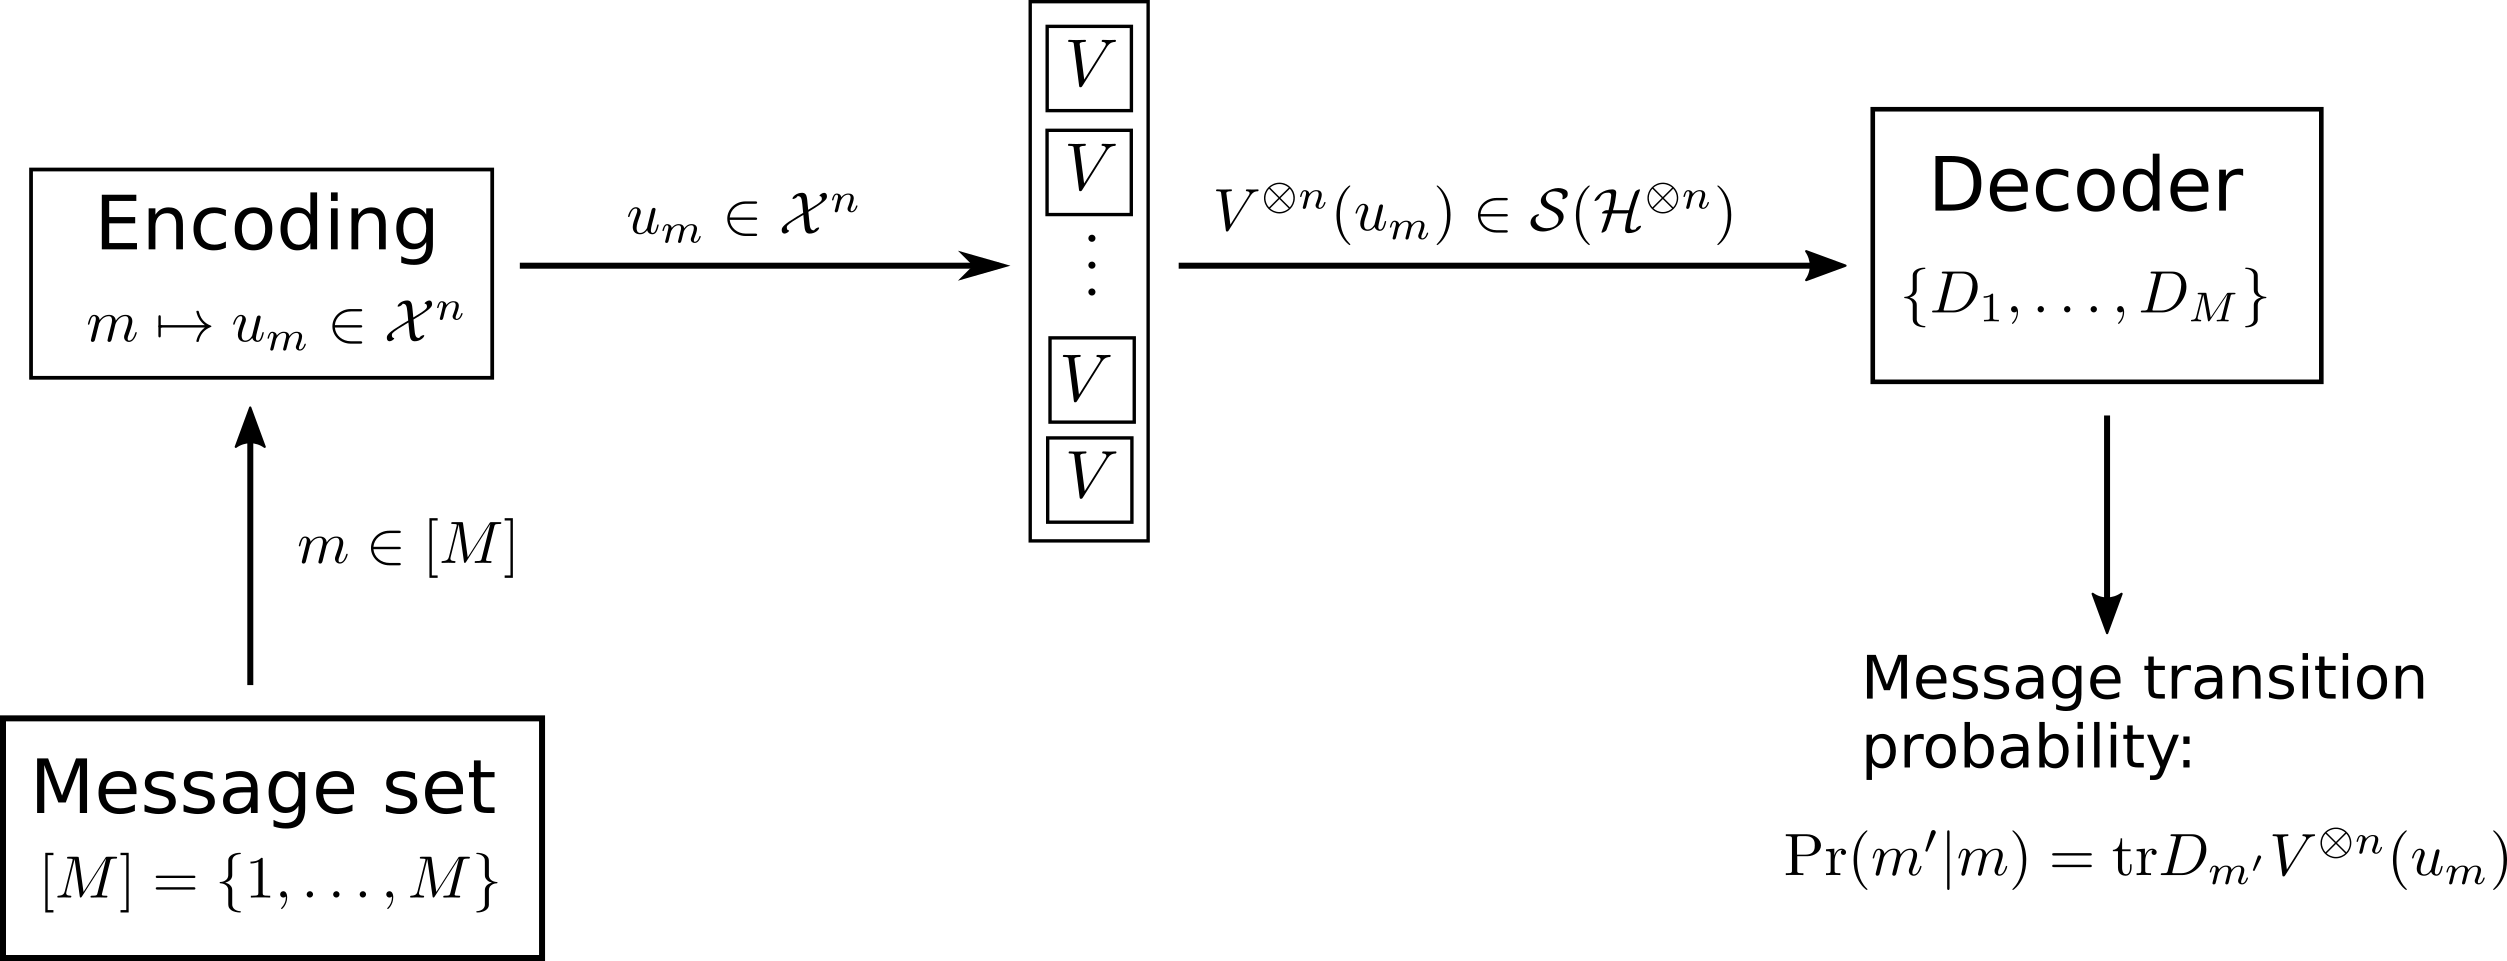
\includegraphics[width=\linewidth]{pics/dmcqc_coding_pic}
		\caption{Coding scheme for classical message transmission over $n$ uses of the DMCQC $V$.}\label{fig:dmcqc_coding_pic}
	\end{figure}
	\newpage
	We give rigorous definitions for the coding scenario. 
	\begin{definition} 
		An \emph{$(n,M)$ code for classical message transmission} over the DMCQC generated by $V: \cX \rightarrow \cS(\cH)$ is a family $\cC := (u_m,D_m)_{m=1}^M$, where 
		$u_1,\dots,u_m$ are words in $\cX^n$, and $\{D_m\}_{m=1}^M$ is a POVM in $\cL(\cH^{\otimes n})$. 
		With the shortcut $D_m^c := \bbmeins_{\cH}^{\otimes n} - D_m$, we define the functions
		\begin{align*}
		\overline{e}(\cC, V^{\otimes n}) \ := \ \frac{1}{M} \sum_{m=1}^M \ \tr D_m^c V^{\otimes n}(u_m)   &&\text{(average transmission error)}, \\
		e(\cC, V^{\otimes n}) \ := \ \underset{m \in [M]}{\max} \ \tr D_m^c V^{\otimes n}(u_m)   &&\text{(maximal transmission error)}.
		\end{align*}
	\end{definition}
	The quantities, which we aim to maximize are, for given transmission error $0 < \lambda < 1$, the maximal size of message sets for each blocklength $n$ which allow transmission error being at most $\lambda$. We define the following quantities accordingly 
	\begin{align*}
	\overline{N}(V,n,\lambda) &:= \max\{M \in \bbmN: \ \exists \ (n,M) \ \text{code} \ \cC \ \text{with} \ \overline{e}(\cC,V^{\otimes n}) \leq \lambda \}, \\
	N(V,n,\lambda) &:= \max\{M \in \bbmN: \ \exists \ (n,M) \ \text{code} \ \cC \ \text{with} \ e(\cC,W^{\otimes n}) \leq \lambda \}.
	\end{align*}
	The quantities defined above grow in general exponentially with $n$ (except, when the channel is completely useless for message transmission). We will determine the asymptotic behaviour of the \emph{transmission rates} 
	\begin{align*}
	\frac{1}{n}\log N(V,n,\lambda), \hspace{.3cm} \text{and} \hspace{.3cm} \frac{1}{n} \log \overline{N}(V,n,\lambda).
	\end{align*}
	\begin{exercise}
		Show, that for each $n\in \bbmN, \lambda \in (0,1)$ and each cq channel $V$, the inequality
		\begin{align*}
		N(V,n,\lambda) \leq \overline{N}(V,n,\lambda) \leq  \frac{1}{1-\sqrt{\lambda}} N(V,n,\sqrt{\lambda}) .
		\end{align*}
		holds. Hint: The left inequality follows directly from the definitions. The proof for the right inequality directly carries over from a corresponding relation for classical discrete memoryless channels.
	\end{exercise}
	For characterizing the message transmission capacity of the DMCQC we need the following function.
	\begin{definition}[Holevo quantity]
		Let $V: \cX \rightarrow \cS(\cH)$ be a cq channel and $q \in \cP(\cX)$ a probability distribution. The function
		\begin{align}
		\chi(q,V) := S(\overline{V}_q) - \sum_{x \in \cX} q(x) S(V(x))
		\end{align}
		with $\overline{V}_q := \sum_{x \in \cX} q(x) V(x)$ is called the \emph{Holevo quantity} \index{Holevo quantity} of $(q,V)$. 
	\end{definition}
	A convenient equivalent of the above expression can be given in terms of the quantum relative entropy. It holds by definition 
	\begin{align}
	\chi(q,V) = \sum_{x \in \cX} \ q(x) \ D(V(x)||\overline{V}_q). \label{altern_holevo_chi_form}
	\end{align}
	%It holds
	%\begin{align}
	%S(\overline{V}_q) - \sum_{x \in \cX} q(x) S(V(x)) 
	%& \ = \  - \tr\overline{V}_q \log \overline{V}_q - \sum_{x \in \cX} q(x) \tr V(x)\log V(x) \\
	%& \ = \ - \sum_{x \in \cX} q(x)  \tr  \left( V(x) \left( \log \overline{V}_q - \log V(x) \right) \right)
	%\end{align}
	Moreover, the \emph{Holevo Information} \index{Holevo information} of the channel $V$ is defined by
	\begin{align} \index{Holevo information}
	C(V) \ := \ \underset{p \in \cP(\cX)}{\sup} \ \chi(p,V).  \label{def:cq_holevo_information}
	\end{align}
	We will prove 
	\begin{theorem}[Coding Theorem and Converse] \label{thm:cq_capacity_theorem}
		Let $V: \cX \rightarrow \cS(\cH)$ be a cq channel. The following statements are true.
		\begin{enumerate}
			\item $\forall \lambda > 0:$ \ $\liminf_{n \rightarrow \infty} \frac{1}{n} \log N(V,n,\lambda) \ \geq \ C(V)$. \label{thm:cq_capacity_theorem_1}
			\item $\inf_{\lambda > 0}$ \ $\limsup_{n \rightarrow \infty} \frac{1}{n} \log \overline{N}(V,n,\lambda) \ \leq \ C(V)$. \label{thm:cq_capacity_theorem_2}
			%\item $\forall \lambda > 0:$ \ $\limsup_{n \rightarrow \infty} \frac{1}{n} \log \overline{N}(V,n,\lambda) \leq \sup_{p \in \cP(\cX)} \chi(p,V)$ \label{thm:cq_capacity_theorem_3}
		\end{enumerate}
	\end{theorem}
	The first statement in the above theorem is usually called the \emph{coding theorem} for the discrete memoryless classical-quantum channels, and the second claim the \emph{(weak) converse}
	to the coding theorem. \newline 
	Theorem \ref{thm:cq_capacity_theorem} determines the \emph{message transmission capacity} of a DMCQC $V$ by $C(V)$. \newline 
	In fact, the second claim above can be replaced by the stronger statement 
	\begin{enumerate}
		\item [2'.]$\forall \lambda > 0: \ \limsup_{n \rightarrow \infty} \frac{1}{n} \log \overline{N}(V,n,\lambda) \leq \sup_{p \in \cP(\cX)} \chi(p,V)$, \label{thm:cq_capacity_theorem_3}
	\end{enumerate}
	which is usually called the \emph{strong converse} to the coding theorem for the DMCQC. The claim in 2'. does also hold, but we will not give a proof of this statement here. 
	\subsection{The weak converse to the coding theorem}
	In this section, we aim to show the weak converse, i.e. the upper bound in Theorem \ref{thm:cq_capacity_theorem}.\ref{thm:cq_capacity_theorem_2}. To show an instance of a \emph{data processing inequality} for the Holevo quantity, we need 
	\begin{theorem}\label{cptp_monot_q_rel_entr}
		Let $\rho, \sigma \in\cS(\cH)$, and $\cN \in \cC(\cH,\cK)$. It holds
		\begin{align}
		D(\rho||\sigma) \ \geq \ D(\cN(\rho)|| \cN(\sigma)). \label{cptp_monot_q_rel_entr_1}
		\end{align}
	\end{theorem}
	The monotonicity of the quantum relative entropy under c.p.t.p. maps (inequality in Eq. (\ref{cptp_monot_q_rel_entr_1})) is provided with a very natural interpretation by Quantum Stein's Lemma (Theorem \ref{thm:q_stein_lemma}). 
	The relative entropy $D(\cN(\rho)|| \cN(\sigma))$ determines the optimal second kind error rate for quantum hypothesis tests with null hypothesis $\rho$ and alternative hypothesis $\sigma$. This rate cannot be improved by affecting both hypotheses with "noise" (that is action of a c.p.t.p. map $\cN$). This interpretation also is the idea behind the following "information-theoretic" proof of Theorem \ref{cptp_monot_q_rel_entr}
	\begin{proof}[Proof of Theorem \ref{cptp_monot_q_rel_entr}]
		We assume that $\ker \sigma \subset \ker \rho$. Otherwise $D(\rho||\sigma)$ is infinte which makes the inequality in (\ref{cptp_monot_q_rel_entr_1}) trivial. Since $\cN$ is a linear map, it also holds 
		$\ker \cN(\rho) \subset \ker \cN(\sigma)$ which ensures us, that both sides of the inequality in (\ref{cptp_monot_q_rel_entr_1}) are finite. \newline 
		We first show the inequality 
		\begin{align}
		\beta_{\epsilon, n } (\rho, \sigma) \leq \beta_{\epsilon, n } (\cN(\rho), \cN(\sigma))
		\end{align}
		for each $n \in \bbmN, \epsilon > 0$. 
		Let $\cN_\ast$ be the Hilbert-Schmidt adjoint \index{adjoint!of a c.p. map} to $\cN$ (remember Exercise \ref{ex:h_s_adjoint}). Because $\cN_\ast$ is a completely positive and unital map, the image of the set
		\begin{align}
		[0,\bbmeins_\cK^{\otimes n}] := \{a \in \cL(\cK)^{\otimes n}: \ 0 \leq a \leq \bbmeins_{\cK}^{\otimes n} \},
		\end{align}
		is contained in $[0, \bbmeins_\cH^{\otimes n}]$. We can estimate 
		\begin{align}
		\beta_{\epsilon, n}(\cN(\rho), \cN(\sigma)) 
		&= \inf\left\{\tr(\cN(\sigma)^{\otimes n} a): \ a \in [0,\bbmeins_\cK^{\otimes n}] \ \wedge \ \tr(\cN(\rho)^{\otimes n} a) \geq 1- \epsilon\right\} \nonumber \\
		&= \inf\left\{\tr(\sigma^{\otimes n} \cN^{\otimes n}_\ast(a)): \ a \in [0,\bbmeins_\cK^{\otimes n}] \ \wedge \ \tr(\rho^{\otimes n} \cN^{\otimes n}_\ast(a)) \geq 1 - \epsilon \right\} \nonumber \\
		&= \inf\left\{\tr(\sigma^{\otimes n} b): \ b \in  \cN_\ast([0,\bbmeins_\cK^{\otimes n}]) \ \wedge \ \tr(\rho^{\otimes n} b) \geq 1-\epsilon\right\} \nonumber \\
		&\geq \inf\left\{\tr(\sigma^{\otimes n} b): \ b \in  [0,\bbmeins_\cH^{\otimes n}] \ \wedge \ \tr(\rho^{\otimes n} b) \geq 1-\epsilon \right\} \nonumber \\
		& = \beta_{\epsilon, n}(\rho, \sigma).\label{cptp_monot_q_rel_entr_beta}
		\end{align}
		We conclude
		\begin{align*}
		D(\rho||\sigma) 
		& = - \lim_{n \rightarrow \infty} \frac{1}{n} \log \beta_{\epsilon,n}(\rho,\sigma) \\
		& \geq - \lim_{n \rightarrow \infty} \frac{1}{n} \log \beta_{\epsilon,n}(\cN(\rho),\cN(\sigma)) \\
		& = D(\cN(\rho)||\cN(\sigma)).
		\end{align*}
		The inequality above is by (\ref{cptp_monot_q_rel_entr_beta}). Both equalites are by using Quantum Stein's Lemma. 
	\end{proof}
	Before we proceed, we recall some notation from classical information theory. For a stochastic matrix $W: \cX \rightarrow \cP(\cY)$, and probability distribution $p \in \cP(\cX)$, the \emph{mutual information} \index{mutual information!classical} is defined by 
	\begin{align*}
	I(p,W) \ := \ H(pW) - H(W|p),
	\end{align*}
	where $pW \in \cP(\cY)$ is defined by $pW(y) := \sum_{x \in \cX} p(x)W(y|x)$, and 
	\begin{align*}
	H(W|p) := \sum_{x \in \cX } p(x) H(W(\cdot|x)).
	\end{align*}
	If the channel input and output in are regarded as a pair of random variables $(X,Y)$ with 
	distribution $P_{XY}(x,y) = p(x)W(y|x)$, also the notation 
	\begin{align}
	I(X \wedge Y) := H(X) - H(X|Y) \label{rule_class_transinformations}
	\end{align}
	Based on the classical mutual information, we define for each classical-quantum channel $V: \cX \rightarrow \cS(\cK)$ and probability distribution $p \in \cP(\cX)$ the so-called \emph{accessible information} \index{accessible information}
	\begin{align*}
	\vartheta(p,V) := \sup\left\{I(p, \tilde{V}_\cD): \ \cD \ \text{is a (finite-valued)} \ \text{POVM on} \ \cK \right\}
	\end{align*}
	where $\tilde{V}_{\cD}$ is defined as the effective $|\cX| \times |\cY|$ stochastic matrix with the entries being the conditional measurement results if the POVM $\cD :=  \{D_y\}_{y \in \cY}$ is applied on the channel ouputs, i.e. 
	\begin{align}
	\tilde{V}_{\cD}(y|x) := \tr D_yV(x) &&(x,y) \in \cX \times \cY. \label{channel_cod_effect_stoch_mat}
	\end{align}
	The following proposition provides us with data processing inequalities we need for the converse proof.
	\begin{proposition} \label{prop:holevo_bound}
		Let $V : \cX \rightarrow \cS(\cK)$, $p \in \cP(\cX)$. The following claims hold.
		\begin{enumerate}
			\item For each quantum channel $\cN \in \cC(\cK, \cH)$, it holds \label{prop:holevo_bound_1}
			\begin{align*}
			\chi(p,V) \geq \chi(p, \cN \circ V). &&\text{(Data processing inequality)}\label{holevo_dpi}
			\end{align*}
			\item In particular, it holds \label{prop:holevo_bound_2}
			\begin{align*} 
			\chi(p,V) \geq \vartheta(p,V). &&\text{(Holevo bound)}
			\end{align*}
		\end{enumerate}
	\end{proposition}
	\begin{proof}
		To prove the first claim, we consider the cq channel $\cN\circ V: \ \cX \rightarrow \cS(\cH)$ which arises from the concatenation of $V$ and $\cN$, i.e. 
		\begin{align*}
		\cN\circ V(x) = \cN(V(x))  &&(x \in \cX).
		\end{align*}
		Using the alternative formula (\ref{altern_holevo_chi_form}) for the Holevo quantity, we have
		\begin{align*}
		\chi(p,V) \ 
		&= \ \sum_{x \in \cX} \ p(x) \ D(V(x)||\overline{V}_p) \\
		&\geq \sum_{x \in \cX} \ p(x)\  D(\cN(V(x))||\cN(\overline{V}_p)) \\
		&= \sum_{x \in \cX} \ p(x)\  D(\cN(V(x))||\overline{(\cN\circ V)}_p) \\
		&= \chi(p, \cN \circ V).
		\end{align*}
		The first and the last equality above are by (\ref{altern_holevo_chi_form}) together with linearity of $\cN$ (i.e. $\cN(\overline{V}_p)= \overline{(\cN\circ V)}_p$). The inequality is by monoticity of the quantum relative entropy under c.p.t.p. maps (Theorem \ref{cptp_monot_q_rel_entr}). \\
		It remains to prove the second claim. Let $\cD := \{D_y\}_{y \in \cY} \subset \cL(\cK)$ be any POVM with $|\cY| < \infty$. We show the inequality
		\begin{align}
		\chi(p,V) \geq I(p, \tilde{V}_\cD).
		\end{align}
		Define a c.p.t.p. map $\hat{\cD} \in \cC(\cK, \bbmC^{|\cY|})$ by 
		\begin{align*}
		\hat{\cD}(a) := \sum_{y \in \cY} \ \tr(D_y a) \ \ket{e_y} \bra{e_y} &&(a \in \cL(\cK)).
		\end{align*}
		It holds
		\begin{align*}
		\hat{\cD} \circ V(x)  \ 
		&= \ \sum_{y \in \cY} \ \tr(D_y V(x)) \ \ket{e_y} \bra{e_y} \\
		&= \ \sum_{y \in \cY}  \tilde{V}_{\cD}(y|x) \ \ket{e_y} \bra{e_y}.
		\end{align*}
		Therefore, it holds (remember the definition in (\ref{channel_cod_effect_stoch_mat}))
		\begin{align}
		\chi(p,V) \
		& \geq \ \chi(p, \hat{\cD}\circ V) \nonumber \\
		& =  \ S\left(\sum_{x \in \cX} p(x) \sum_{y \in \cY}  \tilde{V}_{\cD}(y|x) \ \ket{e_y} \bra{e_y}\right) - \sum_{x \in \cX} p(x) S\left(\sum_{y \in \cY}  \tilde{V}_{\cD}(y|x) \ \ket{e_y} \bra{e_y}\right) \nonumber \\
		& = \ H(p\circ \tilde{V}_{\cD}) - H(\tilde{V}_{\cD}|p) \label{prop:holevo_bound_shannon}\\
		& =  \ I(p,\tilde{V}_{\cD}). \nonumber 
		\end{align}
		Note, that the equality in (\ref{prop:holevo_bound_shannon}) is true, because the arguments of the von Neumann entropies in the preceding line are in fact in diagonal form. 
		Maximizing over both sides of the above inequality proves the claim, we obtain
		\begin{align*} 
		\chi(p,V) \ \geq \ \sup\{ I(p,\tilde{V}_\cE): \ \cE \ \text{is a finite POVM on} \ \cH\} = \vartheta(p,V).
		\end{align*}
	\end{proof}
      The inequalities shown in the preceding proposition allow proof of some additivity properties of the Holevo quantity. 
      \begin{proposition}\label{prop:holevo-additivity}
       Let $V: \cX \rightarrow \cS(\cK)$, $W: \cY \rightarrow \cS(\cH)$ be classical-quantum channels. The following claims are true
       \begin{enumerate}
        \item $\sup_{p \in \cP(\cX \times \cY)} \ \chi(p, V \otimes W) \ = \ \sup_{q \in \cP(\cX)} \ \chi(q, V) + \sup_{r \in \cP(\cY)} \ \chi(r,W)$. \label{prop:holevo-additivity_1}
        \item For each $n \in \bbmN$, it holds \label{prop:holevo-additivity_2}
        \begin{align*}
         \frac{1}{n} \ \underset{p \ \in \cP(\cX^n)}{sup} \ \chi(p, V^{\otimes n}) \ = \ \underset{q \in \cP(\cX)}{\sup} \ \chi(q,V).
        \end{align*}
       \end{enumerate}
      \end{proposition}

      \begin{proof}
       We first show the ``$\geq$'' inequality in \ref{prop:holevo-additivity_1}. For fixed probability distributions $q \in \cP(\cX),\ r \in \cP(\cY)$, it holds with $q \otimes r$ being the notation for the product distributions to $q,r$
       \begin{align}
        \chi(q,V) + \chi(r,W) \ 
        &= \ S(\overline{V}_q) + S(\overline{W}_r) - \sum_{x \in \cX} \ q(x) S(V(x)) - \sum_{y \in \cY} \ r(y) \ S(V(y)) \nonumber \\
        &= S\left(\overline{V}_q \otimes \overline{W}_r\right) - \sum_{(x,y) \in \cX \times \cY} q \otimes r(x,y) \cdot \left(S(V(x))  + S(W(y))\right) \label{prop:holevo-additivity_s_add}\\
        &= S\left(\overline{(V \otimes W)}_{q \otimes r}\right) - \sum_{(x,y) \in \cX \times \cY} q \otimes r(x,y) S(V \otimes W(x,y)) \nonumber \\
        &= \chi(q \otimes r, V \otimes W). \label{prop:holevo-additivity_3}
        \end{align}
      The equality in (\ref{prop:holevo-additivity_s_add}) above is by additivity of the von Neumann entropy for product states (i.e. the case of equality in Lemma \ref{lemma:von_neumann_subadditivity}). Consequently, we have
      \begin{align}
       \sup_{p \in \cP(\cX \times \cY)} \ \chi(p, V \otimes W) \ 
       &\geq \ \sup_{q \in \cP(\cX)}\sup_{r \in \cP(\cY)} \chi(q \otimes r, V \otimes W) \nonumber \\ 
       &= \ \sup_{q \in \cP(\cX)} \ \chi(q, V) + \sup_{r \in \cP(\cY)} \ \chi(r,W). \label{prop:holevo-additivity_4}
      \end{align}
      The inequality above is by restricting the set for maximization. The equality follows by maximizing over the equality in (\ref{prop:holevo-additivity_3}). \newline 
      To show the reverse inequality, fix a probability distribution
      $p \in \cP(\cX \times \cY)$. We denote the marginal distributions on $\cX$ and $\cY$ deriving from $p$ by $q$ and $r$, i.e. we set
      \begin{align*}
       q(x) := \sum_{y \in \cY} \ p(x,y) \hspace{.3cm} \text{and} \hspace{.3cm} r(y) := \sum_{x \in \cX} \ p(x,y) 
      \end{align*}
      for each $x \in \cX, y \in \cY$. 
      It then holds 
      \begin{align*}
       \tr_{\cH} \overline{(V \otimes W)}_p \ = \sum_{(x,y) \in \cX \times \cY} \ p(x,y) \ \tr_{\cH}(V(x) \otimes W(y))  = \sum_{x \in \cX} \ q(x) \ U(x) = \overline{V}_q.
      \end{align*}
      By an analogous calculation, the equality 
      \begin{align*}
       \tr_{\cK} \overline{(V \otimes W)}_p = \overline{W}_r
      \end{align*}
      becomes clear. By the above equalities and subadditivity of the von Neumann entropy (Lemma \ref{lemma:von_neumann_subadditivity}), it holds
      \begin{align}
       S\left( \overline{(V \otimes W)}_p \right) \ & \leq S(\overline{V}_q) + S(\overline{W}_r).
		\label{holevo_additivity_inbetween_1}
      \end{align}
      Moreover, we have by additivity of the von Neumann entropy for tensor product states
      \begin{align}
       \sum_{(x,y) \in \cX \times \cY} \ p(x,y) \ S(V(x) \otimes W(y))
        &= \ \sum_{(x,y) \in \cX \times \cY} \ p(x,y) \ S(V(x)) + \sum_{(x,y) \in \cX \times \cY} \ p(x,y) \ S(V(y)) \nonumber \\
        &= \ \sum_{x \in \cX } \ q(x) \ S(V(x)) + \sum_{y \cY} \ r(y) \ S(V(y)). 
        \label{holevo_additivity_inbetween_2}
      \end{align}
       Thus
       \begin{align}
        \chi(p, V \otimes W) \
        & = \ S\left(\overline{(V \otimes W)}_p\right) - \sum_{(x,y) \in \cX \times \cY} \ 	p(x,y) \ S(V(x) \otimes W(y)) \nonumber \\
        & \underset{(\ref{holevo_additivity_inbetween_1}),(\ref{holevo_additivity_inbetween_2})}{\leq} \ S(\overline{V}_q) + S(\overline{W}_r) - \sum_{x \in \cX} \ q(x) S(V(x)) - \sum_{y \in \cY} \ r(y) S(W(y)) \nonumber \\
        & = \ \chi(q,V) + \chi(r,W). \label{prop:holevo-additivity_5}
       \end{align}
       Maximisation over the input probability distribution and the corresponding marginals on both sides of the inequality in (\ref{prop:holevo-additivity_5}) leads us to 
       \begin{align*}
        \sup_{p \in \cP(\cX \times \cY)} \ \chi(p, V \otimes W) \ 
       \leq \sup_{q \in \cP(\cX)}\sup_{r \in \cP(\cY)} \chi(q \otimes r, V \otimes W) 
       = \ \sup_{q \in \cP(\cX)} \ \chi(q, V) + \sup_{r \in \cP(\cY)} \ \chi(r,W),
       \end{align*}
      which shows, combined with (\ref{prop:holevo-additivity_5}) the first claim of the proposition. \newline 
      The second claim is readily verified by iteratively using the first claim, i.e. 
      \begin{align*}
         \ \underset{p \ \in \cP(\cX^n)}{\sup} \ \chi(p, V^{\otimes n}) \ 
         & = \underset{q \ \in \cP(\cX)}{\sup} \ \chi(p, V) + \underset{r \ \in \cP(\cX^{(n-1)})}{\sup} \ \chi(p, V^{\otimes (n-1)}) \\
         & = 2 \cdot \underset{q \ \in \cP(\cX)}{\sup} \ \chi(p, V) + \underset{r \ \in \cP(\cX^{(n-2)})}{\sup} \ \chi(p, V^{\otimes (n-2)}) \\
         & \vdots \\
         & = n \cdot \underset{q \ \in \cP(\cX)}{\sup} \ \chi(p, V). 
      \end{align*}
      \end{proof}
      The next lemma is well-known in classical information theory. The proof can be found in any textbook on (classical) information theory.
      \begin{lemma}[Fano's Lemma] \label{lemma:fano} \index{Fano's lemma}
       Let $(X,X')$ be a pair of random variables with values in $\cX$, and $\gamma := \prob(X \neq X')$. It holds
       \begin{align}
        H(X'|X) \ \leq \gamma \log |\cX| + h(\gamma).
       \end{align}
       with $h(t) := -t\log t - (1-t) \log (1-t)$ being the binary Shannon entropy for $t \in (0,1)$. 
      \end{lemma}
      The following proposition directly implies the weak converse statement in Theorem \ref{thm:cq_capacity_theorem} 
      \begin{proposition}\label{prop:weak_converse_inequality}
       Let $V: \cX \rightarrow \cS(\cH)$ be a classical-quantum channel. It holds
       \begin{align}
        \overline{N}(V,n,\lambda) \ \leq \ \exp \left(n \cdot C(V) + n\cdot \lambda \log |\cX| + 1 \right) \label{prop:weak_converse_inequality_1}
       \end{align}
       for each $n \in \bbmN$, $\lambda \in (0,1)$. 
       \end{proposition}
       \begin{proof}
       Let $n \in \bbmN$, $\lambda \in (0,1)$ be arbitrary but fixed. Let $\cC := (u_m,D_m)_{m=1}^M$ be any $(n,M)$-code for classical message transmission over the DMCQC $V$ which fulfills
       \begin{align}
        \overline{e}(\cC, V^{\otimes n}) \leq \lambda.
       \end{align}
       We show, that the right hand side of Eq. (\ref{prop:weak_converse_inequality_1}) is an upper bound on the number of messages in $\cC$. Let $p_{\ast} \in \cP(\cX^n)$ be the equidistribution on the set of codewords of $\cC$, i.e. 
       \begin{align*}
         p_\ast(x^n) := \begin{cases}
             \frac{1}{M} & \text{if}\ x^n \ \text{is a codeword in} \ \cC \\
             0              & \text{otherwise}
            \end{cases}
       \end{align*}
	It holds
	\begin{align}
	 n \cdot \sup_{p \in \cP(\cX)} \ \chi(p,V) \ 
	 & = \ \sup_{q \in \cP(\cX^n)}  \ \chi(q,V^{\otimes n}) \nonumber \\
	 & \geq \chi(p_\ast, V^{\otimes n}) \nonumber \\
	 &\geq \vartheta(p_{\ast}, V^{\otimes n}). \label{prf:weak_converse_inequality_1}
	\end{align}
        The equality above is by Proposition \ref{prop:holevo-additivity}.\ref{prop:holevo-additivity_2}, the last inequality follows from Holevo's bound Proposition \ref{prop:holevo_bound}.\ref{prop:holevo_bound_2}.
        Using the decoding POVM $\cD := \{D_m\}_{m=1}^M$ from $\cC$, we define a stochastic matrix $\tilde{V}_{n, \cD}: \ \cX^n \rightarrow \cP([M])$ defined by entries
        \begin{align*}
            \tilde{V}_{n,\cD}(m|x^n) := \tr V^{\otimes n}(x^n)D_m &&( x^n \in \cX^n, m \in [M]).
        \end{align*}
        Using (\ref{prf:weak_converse_inequality_1}), we obtain
        \begin{align}
         n \cdot \sup_{p \in \cP(\cX)} \ \chi(p,V) \ \geq \ \vartheta(p_{\ast}, V^{\otimes n}) \ = \underset{\cE \ \text{POVM}}{\sup} \ I(p_{\ast}, (\widetilde{V^{\otimes n}})_{\cE}) \ \geq \ I(p_{\ast}, \tilde{V}_{n,\cD}).
         \label{prf:weak_converse_inequality_2}
        \end{align}
	 Let $(X,Y)$ be the pair of random variables defined by 
	 \begin{align*}
	  \prob\left(X = m \ \wedge \ Y = m' \right) \ 
	  &= \tilde{V}_{n,\cD}(m'|x_m) p_{\ast}(x_m). 
	 \end{align*}
      Then, 
      \begin{align}
       I(p_{\ast}, \tilde{V}_{n,\cD}) \ 
       = \ I(X\wedge Y) \nonumber
        \underset{(\ref{rule_class_transinformations})}{=} H(X) - H(X|Y).
      \end{align}
      Because we chose $p_{\ast}$ to be equidistributed, it holds
      $
       H(X) = H(p_{\ast}) = \log M.
      $
       Note, that also 
      \begin{align}
       \gamma := \prob \left(X \neq Y\right) \
       &= \sum_{m=1}^M \sum_{m' \neq m} \ \prob \left(X = m \wedge Y = m' \right) \nonumber \\
       &= \sum_{m=1}^M \sum_{m' \neq m} p^n(u_m) \cdot \tr D_{m'}V^{\otimes n}(u_m) \nonumber \\
       &= \frac{1}{M} \sum_{m=1}^M \tr(\bbmeins - D_{m})V^{\otimes n}(u_m) \nonumber \\
       &= \overline{e}(\cC, V^{\otimes n}) \label{prf:weak_converse_inequality_} \nonumber \\
       &\leq \lambda
      \end{align}
      holds. Using Fano's inequality (Lemma \ref{lemma:fano}) in combination with the above equality, we further bound the right hand side of Eq. (\ref{prf:weak_converse_inequality_2}). In fact, 
      \begin{align*}
       I(p_{\ast}, \tilde{V}_{n,\cD}) \ 
       = \ H(X) - H(X|Y) \
       \geq \log M - \lambda \log M - h(\lambda).
      \end{align*}
      We end up at
      \begin{align*}
       n \cdot \sup_{p \in \cP(\cX)} \chi(p,V) \ \geq \ \log M - \lambda \log M - 1 \geq \log M - \lambda n \log |\cX| - 1,
      \end{align*}
      which can be rearranged to 
      \begin{align*}
       \log M \ \leq \ n C(V) + n \cdot \lambda \log |\cX| + 1.
      \end{align*}
      Since $\cC$ was an arbitrary code with average error bounded from above by $\lambda$, maximising $M$ over all such codes yields the claimed inequality. 
      \end{proof}
     \subsection{The coding theorem}
      In this section, we aim to show the ``achievability part'' of Theorem \ref{thm:cq_capacity_theorem}. The statement follows directly from the claim of the following proposition. 
     \begin{proposition} \label{prop:holevo_coding_theorem}
       Let $W: \cX \rightarrow \cS(\cH)$ be a cq channel. For each $\lambda \in (0,1)$, and $\delta > 0$ there is a number $n_0 := n_0(\lambda,\delta)$, such that for all $n \geq n_0$ the 
       inequality
       \begin{align*}
        \overline{N}(W,n,\lambda) \ \geq \ \exp\left(n(C(V) - \delta) \right)
       \end{align*}
       is true. 
      \end{proposition}
       One of the main "nonclassical" challenges in our proof of Proposition \ref{prop:holevo_coding_theorem} is to replace a matrix product by a sum. The following matrix inequality provides a suitable replacement for the "union bound" which would be used in the corresponding classical proof. 
      \begin{lemma}[Hayashi-Nagaoka inequality] \label{hayashi_nagaoka_ineq}
       Let $a, b \in \cL(\cK)$ be matrices with $0 \leq a \leq \bbmeins_{\cK}$, $b \geq 0$. It holds
       \begin{align}
        \bbmeins_\cK - (a+b)^{-\tfrac{1}{2}} a (a+b)^{-\tfrac{1}{2}} \ \leq 2(\bbmeins_\cK - a) + 4b, \label{hayashi_nagaoka_ineq_1}
       \end{align}
       where $y^{-1}$ is the generalized inverse of $y$.
      \end{lemma}
       \begin{proof}
        We can assume without loosing generality that $a+b$ has full rank. This can be seen as follows. Let $P$ denote projector onto the support of $a+b$. Note, that $P$ as well as $P^\perp := \bbmeins - P$ commute with $a, b, a+b$. The inequality in \ref{hayashi_nagaoka_ineq_1} holds therefore if and only if the inequalities 
        \begin{align}
        P - (a+b)^{-\tfrac{1}{2}} a (a+b)^{-\tfrac{1}{2}}P \ \leq 2P - PaP + 4PbP
        \label{hayashi_nagaoka_ineq_2}
        \end{align}
        and 
        \begin{align}
        P^\perp - P^\perp(a+b)^{-\tfrac{1}{2}} a (a+b)^{-\tfrac{1}{2}}P^\perp \ \leq 2P^\perp - P^\perp aP^\perp + 4P^\perp bP^\perp \label{hayashi_nagaoka_ineq_3}
        \end{align}       
        simultaneously hold. The inequality in (\ref{hayashi_nagaoka_ineq_3}) is in fact the trivial inequality $P^\perp \leq 2P^{\perp}$. 
        The inequality in (\ref{hayashi_nagaoka_ineq_2}) regarded as a matrix inequality on $\supp(a+b)$, i.e. a version of the original inequality in (\ref{hayashi_nagaoka_ineq_1}) where $(a+b)$ has full rank. \newline   
        First, we note, that for given matrices $x,y,w,z$ it holds
        \begin{align*}
         (x-\bbmeins)b(x - \bbmeins) \ = \ xbx - xb -bx + b, 
        \end{align*}
        which with some rearrangements leads us to 
        \begin{align*}
         xbx \ = \ b + (x-\bbmeins)b + b(x - \bbmeins) + (x - \bbmeins)b(x - \bbmeins). 
        \end{align*}
        Moreover, it holds $(w-z)^\ast (w-z) \geq 0$, which implies 
        \begin{align*}
         w^\ast z + z^\ast w \ \leq w^\ast w + z^\ast z.
        \end{align*}
        which applied with $w := \sqrt{y}(x-\bbmeins)$ and $z := \sqrt{y}$ reads 
        \begin{align}
         (x-\bbmeins)b + b(x-\bbmeins) \ \leq \  (\bbmeins - x)b(\bbmeins -x) + b \label{hn_ineq}
        \end{align}
        We set $x := (a+b)^{-\tfrac{1}{2}}$. We have   
        \begin{align*}
         \bbmeins - (a+b)^{-\tfrac{1}{2}} a (a+b)^{-\tfrac{1}{2}}  \ 
         & \ =	\	 \bbmeins - xax \\
         & \ =	\	 x(a+b)x - xax \\
         & \ =	\	 xbx \\
         & \ =	\	 b + w^\ast z + z^\ast w + (x-\bbmeins) b (x - \bbmeins) \\
         & \ \overset{(\ref{hn_ineq})}{\leq}\	 2b + 2(x - \bbmeins) b (x - \bbmeins) \\
         & \ \overset{(*)}{\leq} \	 2b + 2(x-\bbmeins)x^{-2}(x-\bbmeins) \\
         & \ = 	\	 2b + 2(\bbmeins - 2x^{-1} + x^{-2}) \\
         & \ = 	\	 2b + 2(\bbmeins - 2 (a+b)^\frac{1}{2} + a + b) \\
         & \ \overset{(**)}{\leq} \	 2b + 2(\bbmeins - 2 a + a + b) \\
         & \ = 	\	 4b + 2(\bbmeins - 2 a)
         \end{align*}
		 The equalties above are by rearrangement of terms, $(*)$ is by the inequality $b \leq (a+b) = x^{-2}$, and $(**)$ is true, because the map $x \mapsto x^{\frac{1}{2}}$ is matrix monotone, therefore $a \leq a^{-\frac{1}{2}} \leq (a+b)^{-\frac{1}{2}}$.
       \end{proof}
     Let $V: \cX \rightarrow \cS(\cH)$ be a classical-quantum channel, and $q \in \cP(\cX)$ be a probability distribution. We define density matrices $\rho(p,V)$ and $\sigma(p,V)$ on $\bbmC^{|\cX|} \otimes \cH$ by
      \begin{align}
       \rho(p,V) \ &:= \ \sum_{x \in \cX} q(x) \ket{e_x} \bra{e_x} \otimes V(x) \label{channel_cq_state_1}\\
       \sigma(p,V) \ &:= \ \sum_{x \in \cX} q(x) \ket{e_x} \bra{e_x} \otimes \overline{V}_q,      
       \label{channel_cq_state_2}
      \end{align}
      where we again used the definition $\overline{V}_q := \sum_{x \in \cX} V(x)$.
      \begin{exercise} \label{ex:cq_states_holevo_chi}
       Show, that for $V: \cX \rightarrow \cS(\cH)$, and $q \in \cP(\cX)$
       \begin{align*}
       \chi(q,V) \ = \ D(\rho(q,V)||\sigma(q,V))
       \end{align*}
       holds for the states defined in (\ref{channel_cq_state_1}) and (\ref{channel_cq_state_2}). Hint: Realise, that both matrices can be written as a Block-diagonal matrix, then use the definition of $D(\cdot||\cdot)$. 
      \end{exercise}

      \begin{proposition}[Random coding] \label{prop:coding_from_stein}
       Let $V: \cX \rightarrow \cS(\cH)$ be a classical-quantum channel, and $q \in \cP(\cX)$. Assume, we find for given $n \in \bbmN$, $\lambda \in (0,1)$, $\tau > 0$ an effect $a \in \cL(\cH \otimes \bbmC^{|\cX|})^{\otimes n}$, 
       $0 \leq a \leq \bbmeins_{\cH \otimes \bbmC^{|\cX|}}^{\otimes n}$ which fulfills the conditions
       \begin{enumerate}
        \item $\tr a \rho(q,V)^{\otimes n} \ \geq 1 - \lambda$ and 
        \item $\tr a \sigma(q,V)^{\otimes n} \leq \tau$. 
       \end{enumerate}
	Then there exists for each $M \in \bbmN$ an $(n,M)$-code $\cC = (u_m, D_m)_{m=1}^M$ with
	\begin{align*}
	 \overline{e}(\cC, V^{\otimes n}) \ < \ 2 \lambda + 4M\tau.
	\end{align*}
      \end{proposition}
      \begin{proof}
      Fix $n \in \bbmN$. We set shortcuts $\rho:= \rho(q,V)$, and $\sigma := \sigma(q,V)$. Let 
      \begin{align*}
          v: \ \left(\bbmC^{|\cX|} \otimes \cH)^{\otimes n}\right){\otimes n} \ \rightarrow \ (\bbmC{|\cX|})^{\otimes n} \otimes \cH^{\otimes n} 
      \end{align*}
	be the isometric linear matrix, which permutes the tensor factors in a way, that 
      \begin{align*}
		v\left(\bigotimes_{i=1}^{n}(a_i \otimes b_i)\right) \ = \ \left(\bigotimes_{i=1}^n a_i \right) \otimes \left( \bigotimes_{i=1}^n b_i \right)
      \end{align*}
      for all $a_1,\dots,a_n \in \bbmC{|\cX|}, \ b_1,\dots,b_n \in \cH$. We will use permuted versions of $\rho$, and $\sigma$ defined by 
      \begin{align*}
       \hat{\rho}_n \ 
       &:= \ v \rho^{\otimes n} v^\ast \ = \ \sum_{x^n \in \cX^n} q^n(x^n)  \ket{e_{x^n}}\bra{e_{x^n}} \otimes  V^{\otimes n}(x^n) \\
       \hat{\sigma}_n 
       &:= \ v \sigma^{\otimes n} v^\ast \ = \ \sum_{x^n \in \cX^n} q^n(x^n)  \ket{e_{x^n}}\bra{e_{x^n}} \otimes  \overline{V}_q^{\otimes n} 
      \end{align*}
      with $\hat{a} := vav^\ast$, $\hat{a}$ can without loosing generality be assumed to be of the form
      \begin{align}
       \hat{a} \ = \ \sum_{x^n \in \cX^n} \ket{e_{x^n}}\bra{e_{x^n}} \otimes h_{x^n} \label{decoding_test_cq}
      \end{align}
      with matrices $0 \leq h_{x^n} \leq \bbmeins_{\cH}^{\otimes n}$ (why?). We have
      \begin{align*}
      \tr \hat{a} \hat{\rho}_n \ &= \ \tr a \rho^{\otimes n} \ \geq 1 - \lambda, \ \text{and} \\
      \tr \hat{a} \hat{\sigma}_n \ &= \ \tr a \sigma^{\otimes n} \ \leq \tau. 
      \end{align*}
	  Let, for a fixed number $M \in \bbmN$, $U := (U_1,\dots,U_M)$ be an independent and identically distributed family of random variables, each with values in $\cX^n$ and 
	  \begin{align*}
		  \Pr\left(U_1 = x^n\right) \ = \ q^n(x^n)		
	  \end{align*}
      for all $x^n \in \cX^n$. Each outcome $u = (u_1,\dots,u_M)$ of $U$ is assumed to be a 
      family of codewords and we define an $(n,M)$ code by introducing a decoding POVM       setting 
      \begin{align*}
       \tilde{h}(u) := \sum_{m=1}^M h_{u_m}
      \end{align*}
      with $h_{x^n}$ being the corresponding effect from (\ref{decoding_test_cq}) for each $x^n \in \cX^n$. We define  
      \begin{align*}
       D_{m}(u) \ := \tilde{h}(u)^{-\frac{1}{2}}h_{u_m}\tilde{h}^{-\frac{1}{2}}(u)
      \end{align*}
      (note that we may possibly make use of the pseudoinverse in the above formula). 
      The definitions above assure us, that $\{D_m\}_{m=1}^M$ is indeed a POVM (check this!), which makes $\cC(u) :=  (u_m, D_m(u))_{m=1}^M$ a proper $(n,M)$ classical message transmission code. We will now show, that the expectation of the random code fulfills 
      \begin{align}
      \bbmE\overline{e}(\cC, V^{\otimes n}) \ < \ 2 \lambda + 4M\tau. \label{hayashi-nagaoka-absch}
      \end{align}
      We apply Lemma \ref{hayashi_nagaoka_ineq} for fixed $u = (u_1,\dots, u_M)$, and $m \in [M]$ with the correspondences
	  \begin{align*} 
	   a \ \leftarrow \ h_{u_m} \hspace{.2cm} \text{and} \hspace{.4cm} b \ \leftarrow \ \tilde{h}(u) - h_{u_m} = \sum_{l \neq m} h_{u_l}.
	  \end{align*}
	   The conclusion of Lemma \ref{hayashi_nagaoka_ineq} yields
		\begin{align*}
		 D^c_m(u) \ \leq 2 (\bbmeins - h_{u_m}) + 4 \cdot \sum_{l \neq m} h_{u_l} 
		\end{align*}
		Which via monotonicity of the trace under the L\"owner partial order implies the bound
		\begin{align}
		\tr\left(D_m^c(u)V^{\otimes n}(u_m)\right) \ 
		\leq \ 2 \cdot \tr\left((\bbmeins - h_{u_m})W^{\otimes n}(u_m)\right) \
		+ \ 4 \cdot \sum_{l \neq m} \tr(h_{u_l}V^{\otimes n}). \label{hayashi-nagaoka-consequence}
		\end{align}
	 	Combining the definition for the code average error and the bounds in (\ref{hayashi-nagaoka-consequence}) together with linearity and monotonicity of the expectation, we arrive at
		\begin{align}
		 \bbmE_{U}\left[\overline{e}(\cC(U), V^{\otimes n})\right] \ 
		 &=  \ \frac{1}{M} \sum_{m=1}^M \bbmE_{U}\left[\tr D_m^c(U) V^{\otimes n}(U_m)\right] \nonumber \\
		 &\leq  \ \frac{1}{M} \sum_{m=1}^M \left\{2 \cdot \bbmE_{U_m}\left[\tr(\bbmeins - h_{U_m})V^{\otimes n}(U_m)\right] + 4 \cdot \sum_{l \neq m} \bbmE_{U}\left[\tr h_{U_l}V^{\otimes n}(U_m) \right] \right\} \nonumber \\
		 &=  \ \frac{1}{M} \sum_{m=1}^M \left\{2 \cdot \Delta_m + 4 \sum_{l \neq m}\cdot \Lambda_{lm} \right\}. \label{hayashi-nagaoka-absch-0}
		\end{align}		
		The last line above is just from setting the abbreviations 
		\begin{align*}
		\Delta_m \ := \ \bbmE_{U_m}\left[\tr(\bbmeins - h_{U_m})V^{\otimes n}(U_m)\right] \hspace{.4cm} \Lambda_{lm} \ := \ \bbmE_{U}\left[\tr h_{U_l}V^{\otimes n}(U_m) \right]
		\end{align*}
  		for each $m \in [M]$, $l \neq m$. We bound the terms separately. 
  		\begin{align}
  		 \Delta_m \ 
  		 &= \ 1 - \bbmE_{U_m}\left[\tr h_{U_m} V^{\otimes n}(U_m) \right] \nonumber \\
  		 &= \ 1 - \sum_{x^n \in \cX^n} q^n(x^n) \ \tr h_{x^n}V^{\otimes n}(x^n) \nonumber \\
  		 &= \ 1 - \sum_{x^n,y^n \in \cX^n} q^n(y^n) \cdot \tr \left((\ket{e_{x^n}}\bra{e_{x^n}} \otimes h_{x^n})(\ket{e_{y^n}}\bra{e_{y^n}} \otimes V^{\otimes n}(y^n) \right) \nonumber \\
  		 &= \ 1 - \tr \underbrace{\left(\sum_{x^n \in \cX^n}\ket{e_{x^n}}\bra{e_{x^n}} \otimes h_{x^n}\right)}_{= \ \hat{a}} \underbrace{\left(\sum_{y^n \in \cX^n} q^n(y^n)\ket{e_{y^n}}\bra{e_{y^n}} \otimes V^{\otimes n}(y^n) \right)}_{= \ \hat{\rho}}  \nonumber \\ 
  		 &= \ \tr \hat{a}\hat{\rho} \ \leq \lambda \label{hayashi-nagaoka-absch_1}
  		\end{align}
		The second equality above is by explicitly carrying out the expectation. For the remaining terms we have
		\begin{align}
		 \Lambda_{lm} \ 
		 :&= \ \bbmE_{U}\left[\tr h_{U_l}V^{\otimes n}(U_m) \right] \nonumber \\
		 &= \ E_{U_mU_l}\left[\tr h_{U_l}V^{\otimes n}(U_m)\right] \nonumber \\
		 &= \ \sum_{x^n,y^n \in \cX^n} q^n(x^n)q^n(y^n) \cdot \tr h_{x^n}V^{\otimes n}(y^n) 
		 \nonumber \\
		 &= \ \sum_{x^n \in \cX^n} q^n(x^n) \cdot \tr h_{x^n}\overline{V}_q^{\otimes n} \nonumber \\
		 &= \ \sum_{x^n, z^n \in \cX^n} q^n(x^n) \cdot \tr\left(\ket{e_{z^n}}\bra{e_{z^n}} \otimes h_{z^n}\right)\left(\ket{e_{x^n}}\bra{e_{x^n}} \otimes \overline{V}^{\otimes n}  \right) \nonumber \\ 
		 &= \tr\hat{a}\hat{\sigma}  \ \leq \tau. \label{hayashi-nagaoka-absch_2}
		 \end{align}
		 Using the estimates in (\ref{hayashi-nagaoka-absch_1}) and (\ref{hayashi-nagaoka-absch_2}) to further upper bound the right hand side of (\ref{hayashi-nagaoka-absch-0}), we obtain the inequality in (\ref{hayashi-nagaoka-absch}). As a consequence, we know, that there exists a realization $u'$, such that with the code $\cC := \cC(u')$ the conclusion $\overline{e}(\cC, V^{\otimes n}) < 2 \lambda + 4M\tau$ of the proposition is valid. 
       \end{proof}		
       \begin{proof}[Proof of Proposition \ref{prop:holevo_coding_theorem}]
        To prove the coding theorem, we use the construction in Proposition \ref{prop:coding_from_stein} together with Quantum Stein's Lemma (Theorem \ref{thm:q_stein_lemma}). Fix numbers $\mu \in (0,1), \delta > 0$ and a probability distribution $q \in \cP(\cX)$ sufficient for 
        \begin{align}
        \chi(q,V) \ \geq \ C(V) - \frac{\delta}{4}  \label{near_holevo_information}
        \end{align}
   		 Applying Theorem \ref{thm:q_stein_lemma} with hypotheses $\rho := \rho(q,V)$ and $\sigma := \sigma(q,V)$ (the states from (\ref{channel_cq_state_1}), (\ref{channel_cq_state_2})), 
	   
   		it is clear, that there exists a number $n_0$ such that for all $n > n_0$ we find a test $a_n \in [0,\bbmeins^{\otimes n}]$ which fulfills 
   		\begin{align}
   		 \tr a_n \rho^{\otimes n} \ \geq 1 - \mu \hspace{.4cm} 
   		 \text{and} \hspace{.4cm}
   		 \tr a_n \sigma^{\otimes n} \ \leq \tau_n
   		\end{align}
		with 
		\begin{align}
		 \tau_n \ \leq \ 2^{-n(D(\rho||\sigma) - \frac{\delta}{2})} \ = \ 2^{-n(\chi(q,V) -  \frac{\delta}{2})} \ \leq \ 2^{-n (C(V) - \frac{3}{4}\delta)}
		\end{align}
		The equality above is by the identity from Exercise \ref{ex:cq_states_holevo_chi}, the rightmost inequality by the choice of $q$, i.e. (\ref{near_holevo_information}). Applying Proposition \ref{prop:coding_from_stein} with $a_n$, and $M$ defined by
		\begin{align*}
		2^{n(C(V) - \frac{\delta}{4})} \ \geq \ M \ := \ \lfloor 2^{n(C(V)- \frac{\delta}{4})} \rfloor \ \geq \ 2^{n(C(V)- \delta)}
		\end{align*}
		we know, that there exists an $(n,M)$ code $\cC_n$ with 
		\begin{align*}
			\overline{e}(\cC, V^{\otimes n}) \ 
			&\leq \ 2 \mu + 4 M \tau_n  \nonumber \\ 
			&\leq 2 \mu + 4 \cdot 2^{-n \frac{\delta}{2}}.
		\end{align*}
		Setting for given $\lambda \in (0,1)$ we know, from the above reasoning with $\mu = \lambda/2$, that 
		\begin{align*}
		 \overline{N}(n,V,\lambda) \ \geq \ 2^{n(C(V)-\delta)} 
		\end{align*}
		for each large enough $n$. 
   		\end{proof}	
   	\end{section}
     
     \section{The discrete memoryless quantum channel} \label{sect:dmqc_coding}
     In this section, we consider the task of classical message transmission for memoryless quantum channels, which take quantum systems as inputs (and outputs quantum systems.) The noise characteristics of such a channel is completely described
     by a c.p.t.p. (which explains, why such maps are also called ``quantum channels''.) 
     \begin{definition}
      Let $\cN \in \cC(\cH, \cK)$ be a c.p.t.p. map. The \emph{discrete memoryless quantum channel (DMQC)} generated by $\cN$ is the family
      \begin{align}
       \{\cN^{\otimes n}: n \in \bbmN \}.
      \end{align}
     The transmission map for $n$ uses of the DMQC $\cN$ is $\cN^{\otimes n}$. 
     \end{definition}
     Next we define message transmission codes for DMQCs. 
     \begin{definition} 
     An $(n,M)$-code for transmission of classical messages over the DMQC $\cN \in \cC(\cH,\cK)$ is a family $\cC = (W(m), D_m)_{m=1}^M$ with
     \begin{align*}
      W(m)  & \in \cS(\cH^{\otimes n}), \hspace{.4cm} \text{and} \\
      D_m   & \in [0, \bbmeins_{\cK}^{\otimes n}] \ \text{for all} \ m \in [M] \ \text{and} \sum_{m=1}^M D_m = \bbmeins_{\cK}^{\otimes n}.
     \end{align*}
     We define the \emph{average transmission error} by 
     \begin{align}
      \overline{e}(\cC, \cN^{\otimes n}) := \frac{1}{M} \sum_{m=1}^M \tr D_m^c \cN^{\otimes n}(W(m)),
     \end{align}
     where we again use the notation $D_m^c := \bbmeins_{\cH}^{\otimes n} - D_m$ for each $m \in [M]$.
     \end{definition}
      As in the case of memoryless classical-quantum channels, we will determine the optimal asymptotical rates for classical message transmission. Therefore, we define for given c.p.t.p. map $\cN$ and each
      $\lambda \in [0,1]$, $n \in \bbmN$
     \begin{align*}
      \overline{N}(\cN, n, \lambda) \ := \ \max \left\{M: \ \exists  \ (n,M)-\text{message transmission code}\ \cC \ \text{with}\ \overline{e}(\cC, \cN^{\otimes n}) \leq \lambda \right\}.  
     \end{align*}
     \begin{exercise}[Maximal error] 
      In the above definition, we only defined the average transmission error. Define a corresponding maximal error function, and optimal message set sizes $N(\cN,n, \lambda)$. Show, that 
      \begin{align*}
        (1 - \lambda^2) \overline{N}(\cN, n, \lambda^2) \ \leq \ N(\cN, n, \lambda) \ \leq \ \overline{N}(\cN, n, \lambda)
      \end{align*}
      holds.
     \end{exercise}
     \begin{exercise} \label{ex:message_set_monotonicity}
      Show, that for each $\lambda \in (0,1)$
      \begin{align*}
       \overline{N}(\cN, m, \lambda) \leq \overline{N}(\cN, n, \lambda)
      \end{align*}
      holds, if $m \leq n$.
     \end{exercise}
      Let $\cN \in \cC(\cH,\cK)$. Define for each $k \in \bbmN$, 
		\begin{align} 
		C^{(1)}(\cN^{\otimes k}) \ := \ \sup \{\chi(p, \cM \circ V): \ |\cY| < \infty, \ p \in \cP(\cY), \ V: \cY \rightarrow \cS(\cH^{\otimes k}) \} \label{thm:dmqc_channel_coding_one_shot}.
	\end{align}
		We set 
		\begin{align}
		 C(\cN) := \sup_{k \in \bbmN} \frac{C^{(k)}(\cN^{\otimes k})}{k} \label{def:holevo_information_quantum}
		\end{align}
	Next we state the coding theorem and converse for classical message transmission over quantum discrete memoryless channels. 
    \begin{theorem} \label{thm:dmqc_channel_coding}
    	Let $\cN \in \cC(\cH,\cK)$. It holds
      \begin{enumerate}
       \item \label{thm:dmqc_channel_coding_1}
        $
        \forall \lambda > 0: \ \underset{n \rightarrow \infty}{\liminf} \frac{1}{n} \log \overline{N}(\cN, n, \lambda) \ \geq \ C(\cN). 
       $
       \item  \label{thm:dmqc_channel_coding_2}
		$
        \underset{\lambda > 0}{\inf} \ \underset{n \rightarrow \infty}{\limsup} \frac{1}{n} \log \overline{N}(\cN, n, \lambda) \ \leq \  C(\cN).
       $
       \end{enumerate}
     \end{theorem}
	Compared to the Holevo information $C(W)$ for a discrete memoryless cq channel defined in (\ref{def:cq_holevo_information}) the above defined capacity function $C(\cN)$ for a quantum DMC is of more complex structure. While $C(W)$ can be evaluated just by a maximisation problem for the generic cq channel $W$, $C(\cN)$ is a so-called \emph{multi-letter formula} \index{multi-letter formula} which means, that one from principle has to solve a separate optimisation problem for each instance $\cN^{\otimes k}$, $k \in \bbmN$. It was for some time a major open question whether or not the problem can be reduced such that $C(\cN) =  C^{(1)}(\cN)$ holds, but eventually an example of a channel $\cN$ with $C(\cN) > \cC^{(1)}(\cN)$ was given. However, discussion of the example is beyond the scope of this course. The expression for $C(\cN)$ can be simplified a bit, i.e. then supremum in 
	(\ref{def:holevo_information_quantum}) can be replaced by a limit
	\begin{proposition}\label{prop:fekete_application}
	 Let $\cN \in \cC(\cH, \cK)$. It holds 
	 \begin{align*}
	 C(\cN) = \lim_{k \in \bbmN} \frac{C^{(k)}(\cN^{\otimes k})}{k}
	 \end{align*}
	\end{proposition}
	To prove the above proposition, we will use the following assertion from real analysis. 	
      \begin{lemma}[Fekete's Lemma]
      Let $(a_n)_{n=1}^\infty$ be a real sequence haveing the property
      \begin{align*}
       a_m + a_n \ \leq \ a_{m+n}
      \end{align*}
      for all $n,m \in \bbmN$. Then 
      \begin{align*}
       \underset{n \in \bbmN}{\sup} \frac{a_k}{k} \leq \underset{k \rightarrow \infty}{\lim} \frac{a_k}{k}.
      \end{align*}
     \end{lemma}
     \begin{proof}[Proof of Proposition \ref{prop:fekete_application}]
	 Define 
	\begin{align}
	a_k := C^{(1)}(\cN^{\otimes k}) && (k \in \bbmN).
	\end{align}
	We first convince ourselves, that the sequence $(\tfrac{1}{k}a_k)_{k=1}^\infty$ is convergent. Notice, that the sequence is bounded. It holds
	\begin{align}
	0 \leq \frac{a_k}{k} \leq  \log \dim \cK.  \label{capacity_function_bounded}
	\end{align}
	The left inequality above is obvious from the definitions (the Holevo quantity is always nonnegative. The upper bound above can be seen as follows. For each $k \in \bbmN$, finite alphabet $\cY$, cq channel
	$V: \cY \rightarrow \cH^{\otimes k}$  and probability distribution $q \in \cP(\cY)$, it holds 
	\begin{align*}
	0 
	\ &  \ \leq \chi(q, \cN^{\otimes k}\circ V) \\
	\ & =  \ S\left(\overline{(\cN^{\otimes k}\circ V)}_q\right) - \sum_{y \in \cY} q(y) S(\cN^{\otimes k} \circ V(y)) \\
	\ & \leq \ S\left(\overline{(\cN^{\otimes k}\circ V)}_q\right) \\
	\ & \leq \log \dim \cK^{\otimes k}  \\
	\ & = \ k \log \dim \cK.
	\end{align*}
	The first equality is by definition of the Holevo quantity using the abbreviation
	\begin{align}
	\overline{(\cN^{\otimes k}\circ V)}_q := \sum_{y \in \cY} q(y) \cN^{\otimes k} \circ V(y),
	\end{align}
	the last inequality is by the principal bound $S(\rho) \leq \log d$ which holds for each density matrix $\rho$ on a $d$-dimensional Hilbert space. Maximizing over all finite alphabets and consistent probability 
	distributions and cq channels leads to the desired upper bound. \\
	Next we show subadditivity of the sequence $(\tfrac{1}{k} a_k)_{k=1}^\infty$, i.e. 
	\begin{align}
	a_m + a_n \leq a_{m+n} \label{capacity_function_subadditivity}
	\end{align}
	for all $n,m \in \bbmN$. The above statement together with the bounds in (\ref{capacity_function_bounded}) show, that the sequence fulfills the conditions of Fekete's Lemma, which implies the desired existence of 
	limit. We show (\ref{capacity_function_subadditivity}). Fix any $m,n \in \bbmN$, finite alphabets $\cY$ and $\cZ$, and classical-quantum channels $V: \cY \rightarrow \cS(\cH^{\otimes n})$, $W: \cZ \rightarrow \cS(\cH^{\otimes n})$.
	It holds 
	\begin{align*}
	\underset{p \in \cP(\cY)}{\sup} \ \chi(p, \cN^{\otimes m}\circ V) \ + \ \underset{q \in \cP(\cZ)}{\sup} \ \chi(p, \cN^{\otimes n} \circ W) 
	\ & = \ \underset{r \in \cP(\cY \times \cZ)}{\sup} \ \chi\left(r, (\cN^{\otimes m} \circ V)\otimes (\cN^{\otimes n} \circ W)\right) \\
	\ & = \ \underset{r \in \cP(\cY \times \cZ)}{\sup} \ \chi\left(r, (\cN^{\otimes (m+n)}) \circ (V\otimes  W)\right)
	\end{align*}
	The first equality above holds by Proposition \ref{prop:holevo-additivity}.\ref{prop:holevo-additivity_1}. Maximzing both sides of the equality above over all cq channels with finite input alphabets and all compatible probability distributions on the corresponding input alphabets leads to 
	\begin{align*}
	a_m + a_n 
	\ & = \ C^{(1)}(\cN^{\otimes m}) + C^{(1)}(\cN^{\otimes n}) \\
	\ & = \ \underset{(p,V)}{\sup} \ \chi(p, \cN^{\otimes m}\circ V) + \underset{(q,W)}{\sup} \ \chi(q, \cN^{\otimes m} \circ W ) \\
	\ & = \ \underset{(p,V)}{\sup} \ \underset{(q,W)}{\sup} \ \chi(q, \cN^{\otimes m + n} \circ (V \otimes W)) \\
	\ & \ \leq \ \underset{(r,Z)}{\sup} \ \chi(r, \cN^{\otimes m + n} \circ Z) \\ 
	\ & = \ a_{m + n}.
	\end{align*}
	Having convinced ourselves, that the hypotheses of Fekete's Lemma are fulfilled, we can conclude, that 
	\begin{align}
	\underset{k \in \bbmN}{\sup} \frac{C^{(1)}(\cN^{\otimes k})}{k} ) =  \underset{k \rightarrow \infty}{\lim} \frac{C^{(1)}(\cN^{\otimes k})}{k} )
	\end{align}
	holds. 
     \end{proof}
     \begin{proof}[Proof of Theorem \ref{thm:dmqc_channel_coding}]
      We first prove the lower bound in Theorem \ref{thm:dmqc_channel_coding}.\ref{thm:dmqc_channel_coding_1}. For this reason fix $\lambda > 0$, $k \in \bbmN$, a finite alphabet $\cY$, a probability distribution $p \in \cP(\cY)$, a classical-quantum channel $V: \ \cY \rightarrow \cS(\cH^{\otimes k})$. 
      We show, that 
      \begin{align*}
       \underset{n \rightarrow \infty}{\liminf} \ \overline{N}(\cN, n \lambda) \ \geq \ \frac{1}{k} \chi(p, \cN^{\otimes k} \circ V)
      \end{align*}
      holds. Maximizing over all entities we fixed leads to the desired inequality. Define the effective cq channel $W_{V,k} \ : \ \cY \rightarrow \cS(\cK^{\otimes k})$ which arises from concatenating the cq channel $V$ with $k$ instances of $\cN$ by
      \begin{align*}
        W_{V,k}(y) \ :=  \ (\cN^{\otimes k} \circ V)(y) = \cN^{\otimes k}(V(y)) &&(y \in \cY).
      \end{align*}
      We first show the inequality
      \begin{align}
       \overline{N}( \cN , k\cdot l , \lambda )  \geq \overline{N}(W_{V,k} ,l, \lambda).  \label{thm:dmqc_channel_coding_proof_message_set_lower}
      \end{align}
      Let $\tilde{\cC} := (y_m, D_m)_{m=1}^M$ be an $(l,M)$-code for $W_{V,k}$. Then $\cC := (V^{\otimes l}(y_m), D_m)_{m=1}^M$ is an $(k \cdot l, M)$-code for $\cN$. Moreover, it holds for each message $m \in [M]$
      \begin{align*}
       \tr D_m^c W_{V,k}^{\otimes l}(y_m)  \ = \tr(\cN^{\otimes k} \circ V)^{\otimes l}(y_m)D_m^c \ = \ \tr D_m^c \cN^{\otimes k \cdot l}(V^{\otimes l}(y_m)).
      \end{align*}
      By arithmetic averaging over all messages, we arrive at
      \begin{align*}
       \overline{e}(\tilde{\cC}, W_{V,k}^{\otimes l}) \ = \ \overline{e}(\cC, \cN^{\otimes k \cdot l}).
      \end{align*}
      We have shown, that we find for each given $(l,M)$ message transmission code for the cq channel $W_{V,k}$ an $(k\cdot l, M)$ message transmission code for the quantum channel $\cN$ of the same average error which implies, by maximizing, 
      the inequality in (\ref{thm:dmqc_channel_coding_proof_message_set_lower}). Now we can bound
      \begin{align*}
       \underset{n \rightarrow \infty}{\liminf} \ \frac{1}{n} \ \log \overline{N}(\cN, n , \lambda) 
       \ &= \ \underset{l \rightarrow \infty}{\liminf} \ \underset{0 \leq r < k}{\min} \ \frac{1}{l \cdot k + r} \ \log \overline{N}(\cN, k \cdot l + r , \lambda)  \\
       \ &\geq \ \underset{l \rightarrow \infty}{\liminf} \ \underset{0 \leq r < k}{\min} \ \frac{1}{l \cdot k + r} \ \log \overline{N}(\cN, k \cdot l , \lambda)    \\
       \ &= \ \underset{l \rightarrow \infty}{\liminf}  \frac{1}{k (l+ 1)} \ \log \overline{N}(\cN, k \cdot l , \lambda)    \\
       \ &= \ \frac{1}{k} \underset{l \rightarrow \infty}{\liminf}  \frac{1}{l+ 1} \ \log \overline{N}(\cN, k \cdot l , \lambda) \\   
       \ &= \ \frac{1}{k} \underset{l \rightarrow \infty}{\liminf}  \frac{1}{l} \ \log \overline{N}(\cN, k \cdot l , \lambda)   \\
       \ &= \ \frac{1}{k} \underset{l \rightarrow \infty}{\liminf}  \frac{1}{l} \ \log \overline{N}(W_{V,k}, l , \lambda) \\
       \ &\geq \frac{1}{k} \ \chi(p, \cN^{\otimes k} \circ V).
       \end{align*}
       The last inequality above is by application of Theorem \ref{thm:cq_capacity_theorem}.\ref{thm:cq_capacity_theorem_1} on the cq channel $W_{V,k}$. It remains to show the upper bound in Theorem 
       \ref{thm:dmqc_channel_coding}.\ref{thm:dmqc_channel_coding_2}. Let $\delta > 0$, and $l_0 \in \bbmN$ an integer large enough such that each $l \geq l_0$ simultaneously fulfills
       \begin{align}
        \left|\underset{k \rightarrow \infty}{\lim} C^{(1)}(\cN^{\otimes k}) - \frac{1}{l} C^{(1)}(\cN^{\otimes l})\right| \leq \frac{\delta}{2}.
       \end{align}
       and $l > \frac{2}{\delta}$. Fix an $l > l_0$ and an $(l,M)$ code for message transmission over $\cN$ $\cC := (W(m),D_m)_{m =1}^M$ with   
       \begin{align*}
        \overline{e}(\cC, \cN^{\otimes l}) \leq \lambda.
       \end{align*}
       Let $q_\ast$ be the equidistribution on the message set. It holds 
       \begin{align*}
        C^{(1)}(\cN^{\otimes l}) 
        \ & = \ \underset{(p,V)}{\sup} \ \chi(p, \cN^{\otimes l} \circ V) \\
        \ & \geq \ \chi(q_{\ast}, \cN^{\otimes l} \circ W) \\
        \ & \geq \ \vartheta(q_{\ast}, \cN^{\otimes l} \circ W) \\
        \ & \geq \ \log M - \lambda \cdot \log M - 1 \\
       \end{align*}
        Combining the estimates, we have 
        \begin{align*}
         \underset{k \rightarrow \infty}{\lim} \frac{1}{k} C^{(1)}(\cN^{\otimes k}) 
         \ & \geq \ \frac{1}{l} C^{(1)}(\cN^{\otimes l}) - \frac{\delta}{2}  \\
         \ & \geq \ (1- \lambda) \frac{1}{l} \log M - \frac{1}{l} - \frac{\delta}{2} \\ 
         \ & \geq \ (1- \lambda) \frac{1}{l} \log M - \delta.
        \end{align*}
        Since the code was arbitrary (beside the error threshold), we obtain by maximizing the message set sizes of all codes which fulfill the error threshold
        \begin{align*}
         \frac{1}{l} \log \overline{N}(\cN,l, \lambda) \ \leq \ \frac{1}{1-\lambda} \left(\underset{k \rightarrow \infty}{\lim} \frac{1}{k} C^{(1)}(\cN^{\otimes k}) + \delta \right)
        \end{align*}
         Consequently, 
         \begin{align*}
           \underset{\lambda > 0}{\inf} \ \underset{l \rightarrow \infty}{\liminf} \ \frac{1}{l} \log \overline{N}(\cN,l, \lambda) \ \leq \ \underset{k \rightarrow \infty}{\lim} \frac{1}{k} C^{(1)}(\cN^{\otimes k}) + \delta. 
         \end{align*}
        Since $\delta$ was an arbitrary positive number, we are done.
        \end{proof}

       % \begin{section}{Supplement I: Capacity Functions}
       %   Caratheodory's Theorem, Examples of Channels, strict subadditivity examples of the Shannon Capacity formula. 
       % \end{section}
     
	%	\begin{section}{Supplement II: Matrix monotonicty}     	
	%	\end{section}
    
     
     
     
     


\part{Some more Topics}

% \chapter{Types and frequency typical sets}
% \label{app:types}
%  \begin{theorem}
 Let $\dim \cK := d$, $\sigma \in \cS(\cK)$, $\delta \in (0, \frac{1}{2})$. For each $k \in \bbmN$ exists a projector 
 $p_{k,\delta}(\sigma)$ such with the following properties. 
 \begin{enumerate}
  \item $p_{k,\delta}(\sigma) \sigma^{\otimes k} \ = \  \sigma^{\otimes k} p_{k,\delta}(\sigma)$.
  \item $\tr(p_{k,\delta}(\sigma)) \ \leq \ \exp\left(k(S(\sigma) + d (\varphi(\delta) + \gamma(k)) \right)$.
  \item $\tr(p_{k,\delta}(\sigma)) \ \geq \ \exp\left(k(S(\sigma) + d (\varphi(\delta) + \gamma(k)) \right)$.
  \item $\tr(p_{k,\delta}(\sigma) \sigma ^{\otimes k}) \geq 1 - \exp(-k(c \delta^2 - d \gamma(k)) )$.
  \item $\exp\left( - k(S(\sigma) + c'(\sigma)\delta)\right) \cdot p_{k,\delta}(\sigma) 
  \ \leq \ p_{k,\delta}(\sigma) \sigma^{\otimes k} p_{k,\delta}(\sigma)$.
  \item $\exp\left( - k(S(\sigma) - c'(\sigma)\delta)\right) \cdot p_{k,\delta}(\sigma) 
  \ \geq \ p_{k,\delta}(\sigma) \sigma^{\otimes k} p_{k,\delta}(\sigma)$,
 \end{enumerate}
  where functions
  \begin{align}
   \varphi&: (0, \tfrac{1}{2}] \rightarrow \bbmR, \ \varphi(t) := -t \log t &(t \in (0, \tfrac{1}{2}) \\
   \gamma &: \bbmN \rightarrow \bbmR_+, \ \gamma(n):= \frac{\log(n+1)}{n} &(n \in \bbmN)
  \end{align}
 and the constant $c'(\sigma) := - \tr(\pi \log \sigma)$ with $\pi$ being the projection onto the support of $\sigma$ where
 used. 
\end{theorem}



\chapter{Transmission of classical messages over quantum channels: revisited}
\label{chap:channel_cod_rev}
 In this chapter, we will go somewhat deeper into the issue of ....

 
     \subsection{Conditionally frequency typical subspaces}
      In this section, we consider an extension of the notion of frequency typical sets from classical information theory to the setting of cq channels. Let $V: \cX \rightarrow \infty$ be a cq channel. We 
      abbreviate $d:= \dim \cH$. To cope with the corresponding notation, we assume that $\cY := \{1,\dots, d\}$. Let 
      \begin{align}
       V(x) = \sum_{y \in \cY} \ \tilde{V}(y|x) \ket{\phi_y(x)} \bra{\phi_y(x)}
      \end{align}
       be a spectral decomposition of $V(x)$ for each $x \in \cX$. To notate the eigenvalue of $V(x)$ belonging to $\phi_y(x)$ by $\tilde{V}(y|x)$ may seem somewhat suggestive, but we have indeed 
       \begin{align}
         \forall y \in \cY:  \ 0 \ \leq \tilde{V}(y|x) \ \leq 1  \hspace{.3cm} \text{and} \hspace{.3cm} \sum_{y \in \cY} \ \tilde{V}(y|x) = 1
       \end{align} 
      for each $x \in \cX$, i.e. the numbers $\{\tilde{V}(y|x) \}_{x \in \cX, y \in \cY}$ are the entries of a stocastic $\cX \times \cY$ matrix $\tilde{V}$. For each $k \in \bbmN$, and $x^k \in \cX^k$, 
      \begin{align}
       V^{\otimes k}(x^k) = \sum_{y^k \in \cY^k} \ \tilde{V}^k(y^k|x^k) \ket{\phi_y^k(x^k)} \bra{\phi_y^k(x^k)}
      \end{align}
       is a spectral decomposition of $V^{\otimes k}(x^k)$, where we used the notation
       \begin{align}
        \tilde{V}^{k}(y^k|x^k) \ = \ \prod_{i=1}^k \tilde{V}(y_i|x_i), \ \text{and} \hspace{.3cm} \phi_{y^k}(x^k) := \phi_{y_1}(x_1) \otimes \cdots \otimes \phi_{y_k}(x_k)
       \end{align}
       for each $x^k = (x_1,\dots,x_k)$, $y^k = (y_1, \dots, y_k)$. We define for each $\delta > 0$, $x^k \in \cX^k$ the \emph{$\delta$-conditional frequency typcial projector to $V$ given $x^k$ by}
       \begin{align}
        p_{V,\delta}(x^k) \ := \ \sum_{y^k \in T_{\tilde{V},\delta}(x^k)} \ket{\phi_{y^k}(x^k)} \bra{\phi_{y^k}(x^k)}.
       \end{align}
       The following theorem provides some bounds for the frequency typical projections.
       \begin{theorem}\label{th:freq_typ_prj_bounds}
        Let $V: \cX \rightarrow \cS(\cH)$ be a classical-quantum channel, $d := \dim \cH$, and $\delta < \frac{1}{d |\cX|}$, $k \in \bbmN$. It holds
        \begin{enumerate}
         \item [1.] $p_{V,\delta}(x^k)V^{\otimes k}(x^k) \ = \ V^{\otimes k}(x^k) p_{V,\delta}(x^k)$ for all $x^k \in \cX^k$
         \item [2.] $\tr p_{V,\delta}(x^k)V^{\otimes k}(x^k) \ \geq 1 - 2^{-k(c \delta^2 - \alpha_1(k))}$
        \end{enumerate}
        For each $q \in \cP(\cX)$, $x^k \in T_{q,\delta}^k$, abbreviating $\overline{V}_q := \sum_{x \in \cX} q(x) V(x)$, it holds
        \begin{enumerate}
         \item [3.] $\tr p_{\overline{V}_q, 2 \delta |\cX|} V^{\otimes k}(x^k) \ \geq \ 1 - 2^{-k(c \delta^2 - \alpha_1(k))}$
         \item [4.] $2^{k(S(V|q) + \alpha_2(k,\delta))} \ \geq \ \tr p_{V,\delta}(x^k) \ \geq \ 2^{k(S(V|q) + \alpha_2(k,\delta))}$
         \item [5.] $2^{-k(S(V|q) - \alpha_3(\delta))} \ \geq \ p_{V,\delta}(x^k)V^{\otimes k}(x^k) p_{V,\delta}(x^k) \ \geq \ 2^{-k(S(V|q) + \alpha_3(\delta))}$
        \end{enumerate}
       \end{theorem}

         
     
     \subsection{The strong converse to the coding theorem}
     In this section, we aim to stregthen the statement from Theorem \ref{thm:cq_capacity_theorem}.\ref{thm:dmqc_channel_coding_2}. We prove the \emph{strong converse} to the coding theorem \ref{thm:cq_capacity_theorem}.\ref{thm:dmqc_channel_coding_1}, which is the statement
     \begin{align}
      \forall \lambda < 1: \ \underset{n \rightarrow \infty}{\limsup} \frac{1}{n} \log N(n, W, \lambda) \ \leq \ \underset{p \in \cP(\cX)}{\sup} \chi(p,W).
     \end{align}
     \begin{subsubsection}{Gentle measurement}
     \begin{lemma}
      Let $\psi, \phi \in \cH$ be unit vectors in $\cH$. Then 
      \begin{align}
       \|\ket{\psi}\bra{\psi} - \ket{\phi}\bra{\phi}\|_1 \ = \ 2 \sqrt{1 - |\braket{\psi,\phi}|^2}.
      \end{align}
     \end{lemma}
     \begin{proof}
     We may write 
     \begin{align}
      \phi = \cos(\theta) \psi + e^{i\varphi} \sin(\theta) \psi^\perp
     \end{align}
     with some $\theta, \varphi \in [0, 2\pi]$. Notice, that
     \begin{align}
      |\braket{\psi,\phi}|^2 = \cos^2 \theta
     \end{align}
     holds. Moreover,
     \begin{align}
      \ket{\phi} \bra{\phi} \ = \ \cos^2 \phi \ket{\psi}\bra{\psi} + \cos \phi \sin \theta e^{i \varphi} \ket{\psi}\bra{\psi^\perp} + e^{i \varphi} \sin \theta \cos \theta \ket{\psi^\perp}\bra{\psi} 
      + \sin^2 \theta \ket{\psi^\perp}\bra{\psi^\perp}.
     \end{align}
      We now writing $A = \ket{\psi}\bra{\psi} - \ket{\phi} \bra{\phi}$ in matrix form (according to $\psi, \psi^\perp$), we have
      \begin{align*}
       A \ = \ \left(\begin{array}{cc} 1 - \cos^2\theta & - e^{-i\varphi} \sin\theta\cos\theta \\
        - e^{i \varphi} \sin \theta \cos \theta & - \sin^2 \theta \end{array}\right)
         \ = \ \left(\begin{array}{cc} \sin^2\theta & - e^{-i\varphi} \sin\theta\cos\theta \\
        - e^{i \varphi} \sin \theta \cos \theta & - \sin^2 \theta \end{array}\right).
      \end{align*}
     The reader may readily verify, that the eigenvalues of $A$ are $a_1 = |\sin \theta|$ and $a_2 := -|\sin \theta|$. We obtain
     \begin{align}
      \|\ket{\psi}\bra{\psi} - \ket{\phi}\bra{\phi}\|_1 \ = \ |a_1| + |a_2|  \ = \ 2 \cdot \sqrt{\sin^2 \theta}  \ =\  2 \cdot \sqrt{1 - \cos^2 \theta} \ = 2 \cdot \sqrt{1 - |\braket{\psi,\phi}|^2}.
     \end{align}
     \end{proof}
     
     \begin{lemma}
      Let $a,b \in \cL(\cH)$, $a, b \geq 0$. Then
      \begin{align}
       \|a - b \|_1 \ \geq \ \|a^{\tfrac{1}{2}} - b^{\tfrac{1}{2}}\|_2^2.
      \end{align}
     \end{lemma}
     \begin{proof}
      Let 
      \begin{align}
        a^{\tfrac{1}{2}} - b^{\tfrac{1}{2}} = \sum_{i=1}^d \mu_i \ket{v_i}\bra{v_i}
      \end{align}
      be a spectral decomposition of the hermitian matrix $a^{\tfrac{1}{2}} - b^{\tfrac{1}{2}}$. It holds
      \begin{align}
       \|a^{\tfrac{1}{2}} - b^{\tfrac{1}{2}}\|_2^2  \ \tr(a^{\tfrac{1}{2}} - b^{\tfrac{1}{2}})^\ast(a^{\tfrac{1}{2}} - b^{\tfrac{1}{2}}) = \sum_{i=1}^d |\mu_i|^2.
      \end{align}
      Define a unitary matrix $u \in \cL(\cH)$ by 
      \begin{align}
       u \ = \ \sum_{i=1}^d \sign(\mu_i) \ket{v_i} \bra{v_i},
      \end{align}
      where 
      \begin{align}
       \sign(x) := \begin{cases} 1  & \text{if} \ x \geq 0 \\ -1& \text{if} \ x < 0 \end{cases}.
      \end{align}
      We have
      \begin{align}
       u(a^{\tfrac{1}{2}} - b^{\tfrac{1}{2}}) = (a^{\tfrac{1}{2}} - b^{\tfrac{1}{2}})u = \sum_{i=1}^d |\mu_i| \ket{v_i}\bra{v_i} = |a^{\tfrac{1}{2}} - b^{\tfrac{1}{2}}|.
      \end{align}
      Since for all $y, z \in \cL(\cH)$, the identity
      \begin{align}
       x^2 - y^2 = \frac{1}{2}\left((x+y)(x-y)+(x-y)(x+y) \right)
      \end{align}
      is valid, we have
      \begin{align}
       \|a - b\|_1 
       \ & = \ \max\left\{|\tr (a-b)w|: \ w \in \cL(\cH), w^\ast w = \bbmeins_\cH \right\} \\
       \ &  \ \geq |\tr (a-b)u| \\
       \ & = \ |\tr ((a^{\tfrac{1}{2}})^2-(b^{\tfrac{1}{2}})^2)u| \\
       \ & = \ \left|\frac{1}{2} \tr(a^{\tfrac{1}{2}} + b^{\tfrac{1}{2}})(a^{\tfrac{1}{2}} - b^{\tfrac{1}{2}}) + \frac{1}{2} \tr(a^{\tfrac{1}{2}} - b^{\tfrac{1}{2}})(a^{\tfrac{1}{2}} + b^{\tfrac{1}{2}})\right| \\
       \ & = \ \left|\tr(a^{\tfrac{1}{2}} + b^{\tfrac{1}{2}})u(a^{\tfrac{1}{2}} - b^{\tfrac{1}{2}}) \right| \\
       \ & = \ \tr(a^{\tfrac{1}{2}} + b^{\tfrac{1}{2}})|a^{\tfrac{1}{2}} - b^{\tfrac{1}{2}}|  \\
       \ & = \ \sum_{i=1}^d |\mu_i| \tr (a^{\tfrac{1}{2}} + b^{\tfrac{1}{2}})\ket{v_i}\bra{v_i} \\
       \ & = \ \sum_{i=1}^d |\mu_i|(\braket{v_i, a^{\tfrac{1}{2}} v_i}  + \braket{v_i, b^{\tfrac{1}{2}} v_i}) \\
       \ & \geq \ \sum_{i=1}^d |\mu_i| \cdot |\braket{v_i, a^{\tfrac{1}{2}} v_i}  - \braket{v_i, b^{\tfrac{1}{2}} v_i}| \\
       \ & \geq \ \sum_{i=1}^d |\mu_i|^2 \\
       \ & = \ \| a^{\tfrac{1}{2}} - b^{\tfrac{1}{2}} \|_2^2.
      \end{align}
      \end{proof}
      \begin{proposition}
       Let $\rho, \sigma \in \cS(\cH)$ be density matrices. It holds
       \begin{align}
        1 - \sqrt{F(\rho,\sigma)} \ \leq \frac{1}{2} \|\rho - \sigma\|_1 \ \leq \ \sqrt{1 - F(\rho,\sigma)}.
       \end{align}
      \end{proposition}
      \begin{proof}
       We first proof the leftmost inequality. It holds
       \begin{align}
        \|\rho -\sigma\|_1 
        \ & \geq \ \|\rho^{\tfrac{1}{2}} - \sigma^{\tfrac{1}{2}}\|_1 \\
        \ & = \ \tr(\rho^{\tfrac{1}{2}} - \sigma^{\tfrac{1}{2}}) \\
        \ & = \ \tr \rho - 2 \tr \rho^{\tfrac{1}{2}}\sigma^{\tfrac{1}{2}} + \tr \sigma \\ 
        \ & = \ 2 \cdot (1 - \tr \rho^{\tfrac{1}{2}}\sigma^{\tfrac{1}{2}}) \\
        \ & \geq  \ 2 \cdot (1 - \| \rho^{\tfrac{1}{2}}\sigma^{\tfrac{1}{2}}\|_1) \\ 
        \ & = \  2 \cdot \left(1 - \sqrt{F(\rho, \sigma)}\right).
       \end{align}
       For the remaining inequality, let $\psi, \phi$ be state vectors of purifications of $\rho, \sigma$ which fulfill 
       \begin{align}
        F(\rho,\sigma) = |\braket{\phi,\psi}|^2.
       \end{align}
       Notice, that such vectors always exist due to Uhlmann's Theorem. We then have
       \begin{align}
        \| \rho - \sigma\|_1 \ \leq \ \|\ket{\phi}\bra{\phi} - \ket{\psi}\bra{\psi}\|_1 = 2 \sqrt{1- |\braket{\phi, \psi}|^2} = 2 \sqrt{1 - F(\rho,\sigma)}.
       \end{align}
       \end{proof}
      \begin{theorem} \label{theorem:gentle_measurement}
        Let $\rho \in \cS(\cH)$, $E \in \cL(\cH)$, $0 \leq E \leq \bbmeins_\cH$. It holds
        \begin{align}
         \|\rho - E^{\tfrac{1}{2}}\rho E^{\tfrac{1}{2}}\|_1 \leq 3 \sqrt{1 - \tr E\rho}.
        \end{align}
        \end{theorem}
        \begin{proof}
         Let $\psi \in \cH \otimes \cH$ be a state vector of a purification of $\rho$. Then 
         \begin{align}
           \psi' := \frac{(E^{\tfrac{1}{2}} \otimes \bbmeins_\cH)\ket{\psi}\bra{\psi}(E^{\tfrac{1}{2}} \otimes \bbmeins_\cH)^\ast}{\sqrt{\braket{\psi, 
           (E^{\tfrac{1}{2}} \otimes \bbmeins_\cH) \psi}}}
         \end{align}
	is state vector to a purification of 
	\begin{align}
	 \rho' := \frac{E^{\tfrac{1}{2}}\rho E^{\tfrac{1}{2}}}{\tr E \rho}.
	\end{align}
        Consequently, we have
        \begin{align}
         F(\ket{\psi}\bra{\psi}, \ket{\psi'}\bra{\psi'}) 
         \ & = \ |\braket{\psi,\psi'}|^2 \\
         \ & = \ \frac{|\braket{\psi,(E^{\tfrac{1}{2}} \otimes \bbmeins_\cH)\psi}|^2}{\braket{\psi,(E^{\tfrac{1}{2}} \otimes \bbmeins_\cH)\psi}} \\
         \ & = \tr \ket{\psi}\bra{\psi}(E^{\tfrac{1}{2}} \otimes \bbmeins_\cH) \\
         \ & = \tr E^{\tfrac{1}{2}}\rho  \\
         \ & \geq \tr E \rho.
        \end{align}
	It follows
	\begin{align}
	 F(\rho,\rho') \ \geq \ F(\ket{\psi}\bra{\psi}, \ket{\psi'}\bra{\psi'}) \ \geq \ \tr E \rho
	\end{align}
        which implies
        \begin{align}
         \|\rho - \rho'\|_1 \ \leq 2 \sqrt{1 - F(\rho,\rho')} \ \leq \ 2 \sqrt{1 - \tr E \rho}.
        \end{align}
        Finally, we can bound
        \begin{align}
         \|\rho - E^{\frac{1}{2}}\rho E^{\frac{1}{2}}\|_1 
         \ &\leq \ \|\rho - \rho' + \rho' -E^{\frac{1}{2}}\rho E^{\frac{1}{2}}\|_1 \\
         \ &\leq \ \|\rho - \rho'\|_1 + \|\rho' -E^{\frac{1}{2}}\rho E^{\frac{1}{2}}\|_1 \\
         \ & \leq \ 2 \sqrt{1 - \tr E \rho} + |1 - \tr E \rho | \cdot \|E^{\frac{1}{2}}\rho E^{\frac{1}{2}}  \|_1 \\
         \ & \leq \ 3 \sqrt{1 - \tr E \rho}.
        \end{align}
        \end{proof}

	\begin{definition}[Shadow]
	Let $\rho \in \cS(\cH)$ be a density matrix, $B \in \cL(\cH)$, $0 \leq B \leq \bbmeins_\cH$, and $\eta \in \bbmR \cap [0,1]$. We call $B$ an \emph{$\eta$-shadow} for
	$\rho$, if 
	\begin{align}
	 \tr B \rho \geq \eta.
	\end{align}
	\end{definition}
	\begin{lemma}[Shadow Lemma] \label{lemma:shadow_lemma}
	 Let $E \in \cL(\cH)$, $0 \leq E \leq \bbmeins_\cH$, $\rho \in \cS(\cH)$ such that $\rho E = E \rho$. Assume that
	 \begin{align}
	  \tr E \rho \geq 1 - \lambda \hspace{.3cm} \text{and} \hspace{.3cm} \mu_1 E \leq  E^{\tfrac{1}{2}} \rho E^{\tfrac{1}{2}} \leq \mu_2 E  \label{lemma:shadow_lemma_1}
	 \end{align}
	does hold for some positive real numbers $\lambda, \mu_1, \mu_2$. Then
	\begin{align}
	 \frac{1- \lambda}{\mu_2} \ \leq \ \tr E \leq \frac{1}{\mu_1}, \label{lemma:shadow_lemma_2}
	\end{align}
        and, for each $0 \leq B \leq \bbmeins_\cH$ which is an $\eta$-shadow for $\rho$, it holds
        \begin{align}
         \tr B \ \geq \ \frac{\eta - \lambda}{\mu_2}. \label{lemma:shadow_lemma_3}
        \end{align}
	\end{lemma}
        \begin{proof}
        Taking traces on both sides of the right hand set of inequalities in (\ref{lemma:shadow_lemma_1}) implies
        \begin{align}
         \mu_1 \tr E \ \leq \ \tr E \rho \ \leq \ \mu_2 \tr E,
        \end{align}
	which implies, in turn, using the inequalities $1 - \lambda \leq \tr E \rho \leq 1$, the inequalities in (\ref{lemma:shadow_lemma_2}). To prove (\ref{lemma:shadow_lemma_3}), we 
	bound
	\begin{align}
	 \mu_2 \tr B \ \geq \ \mu_2 \tr BE \ 
	 & \geq \  \tr B E^{\tfrac{1}{2}} \rho E^{\tfrac{1}{2}} \\
	 & = \tr B \rho - \tr (\rho - E^{\tfrac{1}{2}}\rho E^{\tfrac{1}{2}}) B \\
	 & \geq  \tr B \rho - \tr(\rho - E^{\tfrac{1}{2}}\rho E^{\tfrac{1}{2}}) \\
	 & \geq \eta - (1 - 1 - \lambda)  \\
	 & = (\eta - \lambda).
	\end{align}
	\end{proof}
	Having provided ourselves with the necessary prerequisites, we proceed to prove the strong converse to the coding theorem. We first show, that (subnormalized) codes with all codewords of the same type 
	and small error have suitable upper bounds for their message set sizes. 
	
	\begin{proposition}\label{strong_converse_pre_proposition}
	 Let $W: \cX \rightarrow \cS(\cH)$ be a classical-quantum channel, $n \in \bbmN$, $q \in \cP(\cX)$ a type of sequences in $\cX^n$. Let $\cC_q := (u_m,D_m)_{m=1}^{M_q}$ be a family with 
	 \begin{enumerate}
	  \item $u_m \in T_q^n$ for all $m \in [M_q]$
	  \item $0 \leq D_m \leq \bbmeins_\cH^{\otimes n}$ for all $m \in [M_q]$, and $\sum_{m=1}^{M_q} D_m \leq \bbmeins_{\cH}^{\otimes n}$
	  \item $e_m := \tr D_m^c W^{\otimes n} \leq \lambda$ for all $m \in [M_q]$.
	 \end{enumerate}
	 Then for each $\xi > 0$ there is a number $n_0(\xi,\lambda,W)$ such that for all $n > n_0$ the lower bound
	 \begin{align}
	  M_q \ \leq \ \frac{4}{1 - \lambda}  \exp\left(n(\chi(q,W) + \xi  \right)
	 \end{align}
        is true. 
	\end{proposition}
	\begin{remark}
	 Notice, that the number $n_0$ in the above statement is independent of the chosen type $q$. This will be of some importance when using Proposition \ref{strong_converse_pre_proposition} to prove a strong converse to Holevo's Theorem 
	\end{remark}

	\begin{proof}
	 Set $d := \dim \cH$, and let $\xi > 0$ be fixed. Fix a blocklength $n \in \bbmN$, and a number $\delta > 0$ large enough to simultaneaously fulfill the following three inequalities
	 \begin{align}
	  \exp\left(-n(c \delta^2/2 + \alpha_1(n)/2 - \log3 /n) \right) \  
	  & \leq \ \frac{1-\lambda}{2}, \\ 
	  \alpha_3(\delta) &\leq \xi/2, \\
	  \varphi(2 |\cX| \delta) + \nu(k) &\leq \xi/2d.
	 \end{align}
         We define 
         \begin{align}
          \overline{W}_q := \sum_{x \in \cX} q(x) W(x) \hspace{.4cm} \text{and} \hspace{.4cm} \hat{q} := p_{n,2|\cX|\delta}(\overline{W}_q),
         \end{align}
         where $p_{n,2|\cX|\delta}(\overline{W}_q)$ is the $2|\cX|\delta$-frequency typical projection in $\cH^{\otimes n}$ belonging to the average output state $\overline{W}_q$. Moreover, we set
         \begin{align}
          W_m := W^{\otimes n}(u_m)
         \end{align}
         for each $m \in [M_q]$. We collect some bounds for the above defined Objects, we need later in the proof. By hypothesis, each $u_m$, $m \in [M_q]$ is of type $q$, we have 
         \begin{enumerate}
          \item[(i)] $\tr \hat{q} W_m \ = \ \tr\left(p_{n,2|\cX|\delta}(\overline{W}_q)W^{\otimes n}(u_m)\right) \ \geq \ 1 - 2^{-n(c \delta^2 - \alpha_1(n))}$
          \item[(ii)] $3 \sqrt{1 - \tr \hat{q}W_m} \ \leq \  2^{n(c\delta^2/2 - \alpha_1(n)/2 - \log3/2)}\ \leq \frac{1-\lambda}{2}$
         \end{enumerate}
         where the last inequality above is a consequence of the choice made for $n$, and $\delta$. Define, for each $m \in [M_q]$ the effect 
         \begin{align}
          D'_m := \hat{q}^{\tfrac{1}{2}} D_m \hat{q}^{\tfrac{1}{2}}
         \end{align}
	 (remembering that $\hat{q}$ is a projection. It then holds 
	 \begin{align}
	  \tr D'_m W_m \ 
	  & = \ \tr D_m \hat{q} W_m \hat{q}  \\
	  & = \tr(D_m W_m) - \tr\left(D_m(W_m - \hat{q} W_m \hat{q}\right). \label{strong_converse_pre_proposition_1}
	 \end{align}
         The first term on the right hand side of (\ref{strong_converse_pre_proposition_1}) is bounded by
         \begin{align}
          \tr(D_m W_m) = 1 - \tr(D_m^c W_m) = 1 - e_m \geq 1 -\lambda \label{strong_converse_pre_proposition_1_1}
         \end{align}
	 by hypothesis. For the second term, we have
	 \begin{align}
	  \tr\left(D_m(W_m - \hat{q} W_m \hat{q})\right) 
	  & \leq \tr (W_m - \hat{q} W_m \hat{q}) \\
	  & = \|W_m - \hat{q} W_m \hat{q}\|_1 \\ 
	  &\leq 3 \sqrt{1 - \tr \hat{q} W_m} \\
	  &\leq \frac{1-\lambda}{2}. \label{strong_converse_pre_proposition_1_2}
	 \end{align}
	 The first inequality and the equality above both are by the fact, that $W_m \geq  \hat{q} W_m \hat{q}$ holds. The second inequality is by Lemma \ref{theorem:gentle_measurement}.
	 The last inequality is by our choice of $n$ and $\delta$. Combining the estimates in (\ref{strong_converse_pre_proposition_1_2}) and (\ref{strong_converse_pre_proposition_1_1}) 
	 with the bound in (\ref{strong_converse_pre_proposition_1}), we obtain
	 \begin{align}
	  \tr D'_m W_m \ \geq \frac{1-\lambda}{2}.
	 \end{align}
         Notice, that with $E := p_{W,\delta}(u_m)$, $B := D'_m$ and $\rho := W_m$, the conditions of Lemma \ref{lemma:shadow_lemma} are fulfilled, i.e. by Theorem \ref{th:freq_typ_prj_bounds}, we 
         have
         \begin{align}
          \mu_1 E \ \leq \ E^{\tfrac{1}{2}} \rho E^{\tfrac{1}{2}} \leq \mu_2 E 
         \end{align}
         if we set 
         \begin{align}
          \mu_1 = 2^{-n(S(W|q) + \alpha_3(\delta))} \hspace{.4cm} \text{and} \hspace{.4cm} \mu_2 = 2^{-n(S(W|q) - \alpha_3(\delta))}.
         \end{align}
	 and
	 \begin{align}
	  \tr \rho E = \tr W_m D'_m = \tr W^{\otimes n}(u_m)p_{W,\delta}(u_m) \geq 1 - 2^{-n(c\delta^2 - \alpha_1(n))}.
	 \end{align}
         Consequently, we have
         \begin{align}
          \tr D'_m \
          \ \geq \left(\frac{1-\lambda}{2} - 2^{-n(c\delta^2 -\alpha_1(n))} \right)\cdot \mu_2^{-1} \ 
          \ \geq \frac{1-\lambda }{4} \cdot \mu_2^{-1}.
         \end{align}
	  On the other hand, 
	  \begin{align}
	   \sum_{m=1}^{M_q} \tr D'_m 
	   & = \ \tr\left(\hat{q} \sum_{m=1}^{M_q} D_m \right) \\
	   & \leq \tr \hat{q} \\
	   & = \tr p_{n, 2|\cX|\delta}(\overline{W}_q) \\
	   & \leq 2^{n(S(\overline{W}_q)+ d(\varphi(2 |\cX| \delta) + \nu(n))}.
	  \end{align}
	  Consequently,
	  \begin{align}
	   M_q \cdot \frac{1-\lambda}{4} \cdot 2^{n(S(W|q) - \frac{\xi}{2})} \leq \sum_{m=1}^{M_q} \tr D'_m \leq 2^{n(S(\overline{W}_q) + \frac{\xi}{2}}
	  \end{align}
	  rearrangements in the inequality between the leftmost and rightmost terms above yields 
	  \begin{align}
	   M_q \leq \frac{1 - \lambda}{4} \exp\left(n(S(\overline{W}_q) - S(W|q) + \xi \right)
	  \end{align}
	  which is the claimed upper bound for $M_q$ since $\chi(q,W) = S(\overline{W}_q) - S(W|q)$ by definition of the Holevo quantity. 
	\end{proof}
	We prove the strong converse
	\begin{theorem}
	 Let $W: \cX \rightarrow \cS(\cH)$ be a classical-quantum channel. It holds for all $\lambda \in (0,1)$ 
	 \begin{align}
	  \underset{n \rightarrow \infty}{\limsup} \frac{1}{n} \log N(n,W,\lambda) \leq \underset{p \in \cP(\cX)}{\sup} \chi(p,W).
	 \end{align}
	\end{theorem}
	\begin{proof}
	 Fix $\lambda, \xi \in (0,1)$, and let $n > n_0$ (where $n_0$ is the number in the statement of Proposition \ref{strong_converse_pre_proposition}.) Let $\cC := (u_m, D_m)_{m=1}^M$ 
	 be any $(n,M)$-code for message transmission over $W$ with maximal error bounded by 
	 \begin{align}
	  e(\cC, W^{\otimes n}) \leq \lambda.
	 \end{align}
         Let $\cT$ be the set of types in $\cX^n$, such that at least one codeword in $\cC$ is of that type, i.e. 
         \begin{align}
          \cT \ := \ \left\{q \in \cT(n,\cX): \ T_q^n \cap \{u_m\}_{m=1}^M \neq \emptyset \right\}.
         \end{align}
	 Set 
	 \begin{align}
	  \cM_q := \{m: \ u_m \in T_q^n \}
	 \end{align}
	 It holds obviously $\cM_q \cap \cM_{q'} = \emptyset$ if $q$ and $q'$ are not equal. Moreover, $M = \sum_{q \in \cT} |\cM_q|$.
	 Note, that for each $q \in \cT$, the family $(u_m,D_m)_{m \in \cM_q}$ fulfills the requirements of Proposition \ref{strong_converse_pre_proposition}. Consequently 
	 \begin{align}
	  |\cM_q| \ \leq \ \frac{1 -\lambda}{4} \cdot 2^{n(\chi(q,W) +\xi)} \ \leq \ \frac{1 -\lambda}{4} \cdot 2^{n(\sup_{p \in \cP(\cX)}\chi(p,W) +\xi)}
	 \end{align}
	 Summing up the bound over all $q \in \cT$, we have
	 \begin{align}
	  M 
	  & = \sum_{q \in \cT} |\cM_q| \\
	  & \leq |\cT| \cdot \frac{1 -\lambda}{4} \cdot 2^{n(\sup_{p \in \cP(\cX)}\chi(p,W) +\xi)}\\
	  & \leq (n+1)^{|\cX|} \cdot \frac{1 -\lambda}{4} \cdot 2^{n(\sup_{p \in \cP(\cX)}\chi(p,W) +\xi)}.
	 \end{align}
	  Since the code $\cC$ was an arbitrary code with maximal error not exceeding $\lambda$, we have 
	 \begin{align}
	  N(n,W,\lambda) \ \leq \ \frac{1 -\lambda}{4} \cdot 2^{n(\sup_{p \in \cP(\cX)}\chi(p,W) +\xi)},
	 \end{align}
	  and, 
	  \begin{align}
	  \underset{n \rightarrow \infty}{\limsup} \frac{1}{n} \log N(n,W,\lambda) \leq \underset{p \in \cP(\cX)}{\sup} \chi(p,W).
	 \end{align}
	  which we set out to prove. 
	 \end{proof}
     \end{subsubsection}

    
     
      
     
     
     \subsection{Alternative proofs for the coding theorem}
     
     

\chapter{Message identification over classical-quantum channels}
\label{chap:cq_identification}
 In this lecture, we consider identification of classical messages over discrete memoryless classical-quantum channels. The task of message
\emph{identification} is to distinguish from that of classical message transmission, which we considered in lecture .. The receiver does not 
need an answer to the question 
\begin{align*}
 \text{What was the message?} 
\end{align*}





\begin{definition} \label{def:id_code}
An $(n,N,\lambda_1,\lambda_2)$ \emph{ID code} for the DMCQC $W: \cX \rightarrow \cS(\cH)$ is a family $(Q(\cdot|i), D_i)_{i=1}^N$ such that 
$Q(\cdot|i) \in \cP(\cX^n)$ is a probability distribution on $\cX^n$ and $D_i \in \cL(\cH^{\otimes n})$, $0 \leq D_i \leq \bbmeins$ for all 
$i \in [N]$ such that 
\end{definition}

\begin{definition} \label{def:sim_id_code}
An $(n,N,\lambda_1,\lambda_2)$ \emph{ID code} for the DMCQC $W: \cX \rightarrow \cS(\cH)$ is a family $(Q(\cdot|i), D_i)_{i=1}^N$ such that 
$Q(\cdot|i) \in \cP(\cX^n)$ is a probability distribution on $\cX^n$, $D_i \in \cL(\cH^{\otimes n})$, $0 \leq D_i \leq \bbmeins$ for all 
$i \in [N]$, and $\sum_{i=1}^N D_i$ forms a POVM.
\end{definition}



\chapter{Message transmission over classical-classical-quantum multiple-access channels}
In earlier sections it was already considered a situation, where a sender aims to transmit classical messages to a receiver via a memoryless classical-quantum channel. In this section we extend the communication scenario to include a second sender. \newline 
We assume presence of a cq channel 
\begin{align}
 W: \cX \times \cY \ \rightarrow \cS(\cH)
\end{align}
The \emph{discrete memoryless classical-quantum multiple-access channel} generated by $W$ is the channel model, where the transmission is governed for each blocklength $n$ by the cq channel
\begin{align}
 W^{\otimes n}(x, y) \ := \ \bigotimes_{i=1}^n \ W(y_i, x_i)
\end{align}
for each $x = (x_1,\dots,x_n) \in \cX^n$ and $y = (y_1,\dots,y_n) \in \cY^n$. 
\begin{example}
independent example
\end{example} 
\begin{example}
dependent example
\end{example} 
As demonstrated by the second example above, the inputs of on sender can disturb the other senders signal considerably. 
Below, there is a schematic picture of the general coding scenario in case of a number of $n$ uses of the channel. 
\begin{definition}
An $(n, M_1, M_2)$ \emph{message transmission code} for the MAC $W$ is a family $\cC(u_{1,m_1}, u_{2,m_2} D_{m_1,m_2})_{m_1=1, m_2=1}^{M_1,M_2}$, where $u_{1,1},\dots,u_{1,M_1} \in \cX^n$, $u_{2,1},\dots,u_{2,M_2} \in \cY^n$, and $(D_{m_1,m_2})_{m_1=1,m_2=1}^{M_1,M_2}$ is a POVM on $\cS(\cH)$.
The \emph{(average) transmission error} of $\cC$ defined by 
\begin{align}
 \overline{e}(\cC, W^{\otimes n}) \ := \ \frac{1}{M_1 \cdot M_2} \sum_{m_1=1}^{M_1} \sum_{m_2=1}^{M_2} \tr D_{m_1,m_2}^c W^{\otimes n}(m_1,m_2).
\end{align}
We remember the notation $A^c := \bbmeins - A$. 
\end{definition} 


\begin{definition}
A pair $(R_1,R_2)$ of nonnegative numbers is called an \emph{achievable rate pair} for message transmission over the MAC $W$, if there is a sequence $(\cC_n)_{n \in \bbmN}$, each $\cC_n$ being an $(n,M_{1,n}, M_{2,n})$-code such that 
\begin{enumerate}
	\item $\lim_{n \rightarrow \infty} \ \overline{e}(\cC_n, W^{\otimes n}) \ = \ 0$,
	\item $\liminf_{n \rightarrow \infty} \ \frac{1}{n} \log M_{1,n} \ \geq R_1$, and
	\item $\liminf_{n \rightarrow \infty} \ \frac{1}{n} \log M_{2,n} \ \geq R_2$
\end{enumerate}
We define the \emph{message transmission capacity region} of the MAC $W$ by 
\begin{align*}
 \overline{C}_{MAC}(W) \ := \ \{(R_1,R_2):\ (R_1,R_2) \ \text{achievable message transmission rate pair} \}
\end{align*}
\end{definition}
The assertions in the following proposition are direct consequences from the definitions made. 
\begin{proposition}
For each cq MAC $W$, the capacity region $\overline{C}_{MAC}(W)$ is a compact and convex subset of $\bbmR^2$.
\end{proposition}

\begin{theorem}\label{cq_mac_coding:coding_thm}
Let $W: \cX \times \cY \ \rightarrow \cS(\cH)$ be a cq channel. It holds
\begin{align}
\overline{C}_{MAC}(W) \ = \bigcup_{\substack{p \in \cP(\cX)\\q \in \cP(\cY)}} \cR(p,q),
\end{align}
\end{theorem}
we will prove Theorem \ref{cq_mac_coding:coding_thm} in two portions. Proposition ... formulates the coding theorem, while the converse is Proposition \label{cq_mac_coding:coding_thm}
\begin{proposition}\label{cq_mac_coding:coding_thm}
Let $W: \cX \times \cY \ \rightarrow \cS(\cH)$ be a cq channel. It holds
\begin{align}
\overline{C}_{MAC}(W) \ \supset \bigcup_{\substack{p \in \cP(\cX)\\q \in \cP(\cY)}} \cR(p,q),
\end{align}
\end{proposition}

\begin{proposition}
Let $W: \cX \times \cY \ \rightarrow \cS(\cH)$ be a cq channel. It holds
\begin{align}
\overline{C}_{MAC}(W) \ \subset \bigcup_{\substack{p \in \cP(\cX)\\q \in \cP(\cY)}} \cR(p,q),
\end{align}
\end{proposition}
\begin{proof}
Let $p \in \cP(\cX), q \in \cP(\cY)$ be arbitrary and fixed probability distributions. We show the inclusion $\overline{C}_{MAC}(W) \subset \cR(p,q)$. \newline 
Fix an arbitrary number $\delta > 0$. We show achievability for the rate pair $(R_1, R_2)$,
\begin{align}
 R_1 \ &:= \ I(A;C) - \delta  \\
 R_2 \ &:= \ I(B;C|A) - \delta
\end{align} 
Fix $n \in \bbmN$. We will randomly choose codewords for each sender and use the random coding lemma ... . 
We introduce two independent families of i.i.d. random variables 
\begin{align}
 U &:= (U_1,\dots, U_{M_1}) \; \text{with} \ \prob(U_i = x^n) = p^n(x^n) \; \text{for each} \ x^n \in \cX^n \\
 V &:= (V_1,\dots, V_{M_2}) \; \text{with} \ \prob(V_{i} = y^n) = q^n(y^n) \; \text{for each} \ y^n \in \cY^n. \\
\end{align}
We define for each realization $v$ of $V$ a cq channel
\begin{align}
W_{1,v}: \ \cX^n \ \rightarrow \cS(\cH^{\otimes n}), \; x \mapsto W_{1,y}(x^n) := \frac{1}{M_2} \sum_{m_2=1}^{M_2} W^{\otimes n}(x^n, v_{m_2})
\end{align}
and for each realization $v$ of $V$ a cq channel 
\begin{align}
W_{2,u}: \ \cY^n \ \rightarrow \cS(\cH^{\otimes n}), \; y \mapsto W_{2,x}(y^n) := \frac{1}{M_1}\sum_{m_1=1}^{M_1}  \ket{u_{m_1}}\bra{u_{m_1}} \otimes  W^{\otimes n}(u_{m_1}, y^n)
\end{align}


\end{proof}




\chapter{A Chernov-Hoeffding type Concentration inequality for random matrices}
\label{chap:hoeffding}
 In this section, we prove a matrix generalization of the well-known classical Chernov bound, which reads as follows.

%\begin{theorem}[Scalar Chernov bound] 
% sdfsd
%\end{theorem}




\begin{theorem}[Lieb's Theorem] \label{thm:lieb}
  Let $H \in \bbmH_d$. The matrix trace function
  \begin{align}
    A \mapsto \tr \exp(H+\log A)
  \end{align}
  is concave on $\bbmH_d^{++}$
\end{theorem}

\begin{definition}[Matrix relative entropy] \label{def:matrix_rel_entropy}
  Let $A, B \in \bbmH_d^{++}$. The matrix relative entropy of $(A,B)$ is defined by
  \begin{align}
    D(A||B) \ := \ \tr \left(A(\log A - \log B) - (A-B) \right).
  \end{align}
\end{definition}

Note that the matrix relative entropy defined above is nothing else, than the extension of the quantum relative entropy defined in Def. \ref{def:q_rel_ent} to the set of all
nonnegative matrices (which are invertible). In fact, let $A, B \in \bbmH_d^{++}$, be nonnegative matrices with
\begin{align}
  A  \ = \ \alpha \cdot \rho \hspace{.5cm} \text{and} \hspace{.5cm} B  \ = \ \beta \cdot \sigma
\end{align}
and $\rho, \sigma \in \cS(\bbmC^d)$ full-rank density matrices, then
\begin{align}
  D(A||B) \  & = \ D(\alpha \rho|| \alpha \sigma)                                                                                                   \\
             & = \ \tr(\alpha \rho(\log \alpha \rho) - \log(\beta \sigma)) - \tr(\alpha \rho - \beta \sigma)                                        \\
             & = \ \tr(\alpha \rho(\log \alpha \bbmeins) + \log \rho) - \log(\beta \bbmeins)) - \log(\sigma)) - (\alpha - \beta)                    \\
             & = \ \alpha D(\rho|| \sigma) + \alpha \log \frac{\alpha}{\beta} - (\alpha - \beta).  \label{relation_matrix_quantum_relative_entropy}
\end{align}
In consequence, some important properties of the quantum relative entropy an be concluded to the matrix relative entropy. An example of this fact is the monotonicity under
completely positive and trace preserving maps, which will be the starting point for the rest of the chapter, and was already shown for density matrix arguments in Theorem
\ref{cptp_monot_q_rel_entr}. A restatement for the present case reads as follows.

\begin{corollary}[CPTP Monotonicity of the Matrix relative entropy]
  Let $A, B \in \bbmH_n^++$, $\cN; \cL(\bbmC^n) \rightarrow \cL(\bbmC^m)$ be a c.p.t.p. map. It holds
  \begin{align}
    D(\cN(A)|| \cN(B)) \leq D(A||B)
  \end{align}
\end{corollary}
\begin{proof}
  We have
  \begin{align}
    D(A||B) - D(\cN(A)||\cN(B)) = \alpha (D(\rho||\sigma) - D(\cN(\rho)||\cN(\sigma))) \geq 0.
  \end{align}
  The equality above is by Eq. (\ref{relation_matrix_quantum_relative_entropy}). The inequality follows by positivity of $\alpha$ and Theorem \ref{cptp_monot_q_rel_entr}.
\end{proof}

\begin{theorem}[Joint Convexity of the matrix relative entropy] \label{matrix_relative_entropy_joint_convexity}
  Let $A_1, A_2, B_1, B_2 \in \bbmH_d^{++}$, and $\lambda \in (0,1)$. It holds
  \begin{align}
    D(\lambda A_1 + (1-\lambda) A_2|| \lambda B_1 + (1-\lambda) B_2) \leq \lambda D(A_1||B_1) + (1-\lambda) D(A_2|| B_2)
  \end{align}
\end{theorem}

\begin{proof}
  Define nonnegative matrices
  \begin{align}
    A := \lambda A_1 \ket{e_1}\bra{e_1} + (1-\lambda) A_2 \otimes \ket{e_2}\bra{e_2} \hspace{.5cm} \text{and} \\
    B := \lambda B_1 \ket{e_1}\bra{e_1} + (1-\lambda) B_2 \ket{e_2}\bra{e_2}.
  \end{align}
  We have
  \begin{align}
    D(A||B) = \lambda D(A_1||B_1) + (1 - \lambda) D(A_2||B_2),
  \end{align}
  on the other hand, tracing out the additional systems gives
  \begin{align}
    \tr_{\bbmC^2} A = \lambda A_1 + (1-\lambda) A_2, \ \text{and} \tr_{\bbmC^2} B = \lambda B_1 + (1-\lambda) B_2.
  \end{align}
  In combination, we have
  \begin{align}
    \lambda D(A_1||B_1) + (1-\lambda) D(A_2||B_2) \
     & = \ D(A||B)                                                              \\
     & \geq D(\tr_{\bbmC^2}A|| \tr_{\bbmC^2} B)                                 \\
     & = D(\lambda A_1 + (1 - \lambda) A_2 || \lambda B_1 + (1 - \lambda) B_2).
  \end{align}
  The inequality above is by c.p.t.p. monotonicity of the matrix relative entropy.
\end{proof}

\begin{lemma} \label{lemma:joint_concavity_implies_partial_concavity}
  Let $f: \bbmH_d^{++} \times \bbmH_d^{++} \rightarrow \bbmR$ be jointly concave. The function $\tilde{f}: \bbmH_d^{++} \rightarrow \bbmR$, given by
  \begin{align}
    \tilde{f}(B) = \underset{A \in \bbmH_d^{++}}{\sup} f(A,B) &  & (B \in \bbmH_d^{++})
  \end{align}
  is concave.
\end{lemma}
\begin{proof}
  Fix $\epsilon > 0$. For each $B_1,B_2 \in \bbmH_d^{++}$ exist $A_1, A_2 \in \bbmH_d^{++}$ such that
  \begin{align}
    f(A_1,B_1) & \geq \underset{A \in \bbmH_d^{++}}{\sup} f(A,B_1) - \epsilon = \tilde{f}(B_1) - \epsilon, \ \text{and} \\
    f(A_2,B_2) & \geq \underset{A \in \bbmH_d^{++}}{\sup} f(A,B_2) - \epsilon = \tilde{f}(B_2) - \epsilon
  \end{align}
  For each $\lambda \in (0,1)$, we have
  \begin{align}
    \tilde{f}(\lambda B_1 + (1- \lambda) B_2) \
     & = \ \underset{A \in \bbmH_d^{++}}{\sup} f(A, \lambda B_1 + (1 - \lambda) B_2)          \\
     & \geq \ f(\lambda A_1 + (1-\lambda) A_2, \lambda B_1 + (1 - \lambda) B_2)               \\
     & \geq \lambda f(A_1,B_1) + (1 - \lambda) f(A_2,B_2)                                     \\
     & \geq \lambda (\tilde{f}(A_1) - \epsilon) + (1 - \lambda) (\tilde{f}(B_2) -  \epsilon).
  \end{align}
  Since $\epsilon$ was an arbitrary positive number, we are done.
\end{proof}
\begin{lemma}\label{lemma:trace_variational}
  Let $\bbmM \in \bbmH_d^{++}$. It holds
  \begin{align}
    \tr M = \underset{T \in \bbmH_d^{++}}{\sup} \tr(T \log M - T \log T +T)
  \end{align}
\end{lemma}
\begin{proof}
  By rearrangement of the inequality $D(M||T) \geq 0$, we know, that the l.h.s. of the equality to prove exceeds the r.h.s. On the other hand, equality is attained
  when $T = M$.
\end{proof}
\begin{proof}[Proof of Theorem \ref{thm:lieb}]
  We use Lemma \ref{lemma:trace_variational} with $M := \exp(H + \log A)$ to obtain
  \begin{align}
    \tr \exp (H + \log A) \
     & = \ \underset{T \in \bbmH_d^{++}}{\sup} \tr\left(T( H+ \log A) - T \log T + T \right) \\
     & = \ \underset{T \in \bbmH_d^{++}}{\sup} \tr\left(TH) + \tr(A) - D(T||A) \right).      \\
  \end{align}
  Since the matrix relative entropy is jointly convex, the function
  \begin{align}
    f(T,A) := \tr(TH) + \tr A - D(T||A)
  \end{align}
  is jointly concave. Using Lemma \ref{lemma:joint_concavity_implies_partial_concavity}, and the variational formula above, we are done.
\end{proof}

Next, we aim to prove a chernov-type bound for sums of independent hermitian random matrices. For each hermitian matrix $A \in \bbmH_d$, we use the shorcuts
$\lambda_{\max}(A)$ and $\lambda_{\min}(A)$ to denote the maximal and minimal eigenvalues. It holds
\begin{proposition}
  Let $Y: \Omega \rightarrow \bbmH_d$ be a hermitian random matrix. For all $t \in \bbmR$, it holds
  \begin{align}
    \prob(\lambda_{\max}(Y) \geq t) \  & \leq \ \underset{\theta > 0}{\inf} \ e^{-\theta t} \cdot  \bbmE \tr e^{\theta Y}, \ \hspace{.5cm} \text{and} \\
    \prob(\lambda_{\min}(Y) \leq t) \  & \leq \ \underset{\theta < 0}{\inf} \ e^{-\theta t} \cdot  \bbmE \tr e^{\theta Y}.
  \end{align}
\end{proposition}

\begin{theorem}
  Let $\{X_k\}_{k=1}^N$ be an independent family of hermitian random matrices, $X_k: \Omega \rightarrow \bbmH_d$ ($k \in [N]$). Set $Y := \sum_{k=1}^N X_k$.
  It holds for all $t \in \bbmR$


\end{theorem}




% \chapter{Transmission of private messages over quantum channels}

% \chapter{The genuine quantum capacities}

\chapter{Teleportation and Dense Coding}
\label{chap:telep_dense_cod}
 In this chapter, we consider \emph{teleportation} and \emph{dense coding} two prominent protocols being prominent in quantum information theory. 


\begin{subsection}{Local operations and classical communication}
 We introduce notions which go beyond the concept of quantum channels. 
 
 \begin{definition}[Operation]
  Let $\cH, \cK$ be Hilbert spaces. A completely positive map $\cT: \ \cL(\cH) \rightarrow \cL(\cK)$ which in addition is trace-nonincreasing, i.e. 
  \begin{align}
   \tr \cT(A) \leq \tr A &&(A \in \cL(\cH), A \geq 0)
  \end{align}
  is called \emph{(quantum) operation}. We define the shortcut
  \begin{align}
   \cC^{\downarrow}(\cH, \cK) := \left\{\cT: \cL(\cH) \rightarrow \cL(\cK): \ \cT \ \text{is c.p., and} \ \forall A \geq 0: \ \tr \cT(A) \leq \tr A  \right\}.
  \end{align}
 \end{definition}
 \begin{remark} 
  \begin{enumerate}
   \item [(i)] By definition, a quantum channel (completely positive and trace preserving map) is an operation, i.e. $\cC(\cH,\cK) \subset \ \cC^{\downarrow}(\cH,\cK)$.
   \item [(ii)] Because an operation is c.p. in particular, it admits a Kraus representation.
   \item [(iii)] An operation can be always completed to be a quantum channel by adding a suitable c.p. map.
  \end{enumerate}
 \end{remark}
 
 \begin{definition}[Instrument]
 Let $|\cX| < \infty$. A \emph{(quantum) instrument} is a family $\{\cT_x\}_{x \in \cX}$ such that 
 \begin{enumerate}
  \item $\cT_x \in \cC^{\downarrow}(\cH,\cK)$ for each $x \in \cX$, and
  \item $\sum_{x \in \cX} \cT_x \in \cC(\cH,\cK)$.
 \end{enumerate}
 \end{definition}
 
 \begin{definition}[One-way LOCC channels]
 Let $\cH_A, \cH_B, \cK_A, \cH_B$ be Hilbert spaces of systems under control of communication parties $A$ and $B$. A quantum channel $\cN \in \cC(\cH_A \otimes \cH_B, \cK_A \otimes \cK_B)$ is a LOCC channel with local operations regarding $A$ and $B$ and (noiseless) classical communication from $A$ to $B$ ($A\rightarrow B$-one-way LOCC channel), if it can be written in the form
 \begin{align}
  \cN(a) := \sum_{k=1}^N \cA_k \otimes \cB_k (a) 
 \end{align}
 where $\{\cA_k: k \in [N]\}\subset \cC{\downarrow}(\cH_A, \cK_A)$ is a quantum instrument, and $\cB_k \in \cC(\cH_B,\cK_B)$ is a quantum channel for each $k \in [N]$. 
 \end{definition} 
\end{subsection}
\begin{subsection}{Entanglement-enhanced LOCC - Quantum Teleportation}
It is known, that one cannot exceed the class of separable states by LOCC mappings. A very interesting class of protocols arises, if two parties can use preshared entangled states in addition to local operations and classical communiation. One prominent example of this class is the so-called \emph{quantum teleportation} protocol. 
\begin{theorem}[Quantum teleportation]\label{thm:teleportation} \index{quantum!teleportation}
Let $\cH_A \simeq \cK_A \simeq \cK_B$ be Hilbert spaces. There exists an $A \rightarrow B$ one-way LOCC channel $\cT \in \cC(\cH_A \otimes \cK_A \otimes \cK_B, \cK_B)$ such that with a pure maximally entangled state
$\Phi \in \cS(\cK_A \otimes \cK_B)$
\begin{align}
\cT(a \otimes \Phi) \ = \ a \label{thm:teleportation_1}
\end{align}
for each $a \in \cL(\cH_A)$. 	
\end{theorem}
Before we prove the above assertion, we supply us with the following lemma.
\begin{lemma}\label{lemma:unitary_basis}
Let $d \in \bbmN$. There exists a family $\{v_i\}_{i=1}^{d^2} \subset \cL(\bbmC^d)$ of unitary matrices, such that the following properties hold. 
\begin{enumerate}
	\item $\tr v_i^\ast v_k \ = \ d \delta_{ij}$ for all $i,j \in [d^2]$
	\item With $\phi := \sqrt{d}^{-1} \sum_{k=1}^d e_k \otimes e_k$ and $\phi_i := (v_i\otimes \bbmeins)\phi$ for each $i \in [d]$, it holds  \label{lemma:unitary_basis_2}
	\begin{enumerate}
		\item[\ref{lemma:unitary_basis_2}a.] $\braket{\phi_i, \phi_j}  \ = \ \delta_{ij}$ for all $i,j \in [d]$
		\item[\ref{lemma:unitary_basis_2}b.] $\sum_{i=1}^{d^2} \ket{\phi_i}\bra{\phi_i} \ = \ \bbmeins \otimes \bbmeins$.
	\end{enumerate}
\end{enumerate}
\end{lemma}

\begin{proof}
Let $\gamma: \{0,d-1\} \times \{0,d-1\} \rightarrow [d^1]$ be any bijection. We will show, that the matrices
\begin{align}
v_i := v_{\gamma(r,s)} := \sum_{l=0}^{d-1} e^{-i2\pi s l /d} \ket{e_{l \ominus r}}\bra{e_l} &&(i \in [d^2]) 
\end{align}
suffice the properties claimed in the lemma ($\ominus$ denotes the modulo-$d$ substraction). Unitarity of $v_1,\dots, v_{d^2}$ follows by straightforward calculation. To show the first claim of the lemma, 
let $(r,s) = \gamma{-1}(j)$, $(r',s') = \gamma^{-1}(k)$. It holds
\begin{align}
\tr v_k^\ast v_j \ 
= \ \sum_{l,l'=0}^{d-1} e^{i2\pi'(s'l' - sl)/d} \delta_{r'r}\cdot \delta_{l'l} \
= \ \sum_{l=0}^{d-1} e^{i2\pi(s'-s)l/d}  \delta_{rr'} \label{lemma:unitary_basis_4}
\end{align}
We assume $r = r'$ and evaluate the right hand side of (\ref{lemma:unitary_basis_4}). If $s=s'$, one can directly see, that $j=k$, and 
\begin{align}
\tr_{v_k^\ast v_j} = d.
\end{align}
When $s \neq s'$, then 
\begin{align}
\sum_{l=0}^{d-1} e^{i2\pi(s'-s)l/d} \ = \ \sum_{l=0}^{d-1} (e^{i2\pi(s'-s)/d})^l = 0
\end{align}
To verify the rightmost of the above inequalites, we notice, that evaluating the geometric sum $\sum_l=0^{d-1} q^l$ with $q = e^{i2\pi(s'-s)/d}$ leads us to 
\begin{align}
\sum_{l=0}^{d-1} (e^{i2\pi(s'-s)/d})^l = \frac{1 - e^{i2\pi(s-s')}}{1- e^{(s-s')/d}} = 0.
\end{align}
We summarize
\begin{itemize}
\item $k \neq j \ \Rightarrow \ r \neq r' \vee s \neq s' \ \Rightarrow \tr v_k^\ast v_j = 0$
\item $k = j \ \Rightarrow \ r = r' \wedge s=s' \ \Rightarrow \tr v_k^\ast v_j = d$
\end{itemize}
which shows the first claim. The remaining statements are rather straightforward applications of the first statement and are left as exercises. 
\end{proof}
\begin{proof}[Proof of Theorem \ref{thm:teleportation}]
Let $\dim \cH_A = d$, and $\Phi := \ket{\phi}\bra{\phi}$ with $\phi := \sqrt{d}^{-1} \sum_{k=1}^d e_k \otimes e_k$. Using the family $\{v_i\}_{i=1}^{d^2}$ and the family $\{\phi_i\}_{i=1}^{d^2}$ from lemma \ref{lemma:unitary_basis} respectively, we set $\Phi_k := \ket{\phi_k}\bra{\phi_k}$,
\begin{align} 
 \cE_k(\cdot) \ &:= P_k (\cdot) P_k^\ast \ \in \cC^{\downarrow}(\cH_A \otimes \cK_A, \cH_A \otimes \cK_A)\hspace{.5cm} \text{and} \\
 \cU_k(\cdot) \ &:= v_k(\cdot)v_k^\ast \ \in \cC(\cK_B, \cK_B) 
\end{align}
for each $k \in [d^2]$. It is easy to check, usign the claims of Lemma \ref{lemma:unitary_basis}, that 
$\{\cE_k: \ k \in [d^2]\}$ is a quantum instrument, and consequently
\begin{align}
\tilde{\cT}(\cdot) \ := \ \sum_{k=1}^{d^2} \cE_k \otimes \cU_k(\cdot) \label{thm:teleportation_2}
\end{align}
is an $A\rightarrow B$ one-way LOCC channel. Moreover, the channel $\cT := \tr_{\cH_A \otimes \cK_A} \circ \tilde{\cT}$ is also an $A\rightarrow B$ one-way LOCC channel (Check this!). We show, that $\cT$ 
suffices the identity in (\ref{thm:teleportation_1}). Since the map $a \mapsto \cT(a \otimes \Phi)$ is linear, it is enough to show the identity for all matrix units $E_{ij} := \ket{e_i}\bra{e_j}$, $i,j \in [d]$. With the notation introduced, notice, that 
\begin{align}
\Phi &= \frac{1}{d} \sum_{i,j=1}^d E_{ij} \otimes E_{ij}, \ \text{and} \\
\Phi_k& = \frac{1}{d} \sum_{i,j=1}^d E_{ij} \otimes v_kE_{ij}v_k^\ast &&(k \in [d^2])
\end{align}
holds. We individually evaluate the summands in the right hand side of Eq. (\ref{thm:teleportation_2}). It holds for each $k \in [d^2], m,n \in [d]$
\begin{align}
 \cE_k \otimes \cU_k (E_{mn} \otimes \Phi)  \
 &= \ (\Phi_k \otimes v_k^\ast)(E_{mn} \otimes \Phi) (\Phi_k \otimes v_k^\ast)^\ast \\
 &= \ \frac{1}{d} \sum_{i,j=1}^d (\Phi_k \otimes v_k^\ast) (E_{mn} \otimes E_{ij} \otimes E_{ij})(\Phi_k \otimes v_k^\ast)^\ast \\
 &= \ \Phi_k \otimes \left(\frac{1}{d} \sum_{i,j=1}^d \braket{\phi_k, e_m \otimes e_i}\braket{e_n \otimes e_k, \phi_k} \cdot v_k^\ast E_{ij} v_k\right)
\end{align}
A calculation shows, that the termin in brackets above equals $\frac{1}{d} E_{mn}$. Summing up the equalities, we have
\begin{align}
\cT(\Phi, E_{mn}) \ 
 & = \ \tr_{\cH_A \otimes \cK_A}\left(\sum_{k=1}^{d^2} \cE_k \otimes \cU_k (\Phi \otimes E_{mn}) \right) \\
 & = \ \tr_{\cH_A \otimes \cK_A}\left(\sum_{k=1}^{d^2} \Phi_k \otimes E_{mn}\right) \\
 & = \ E_{mn}.
\end{align}
\end{proof}
\end{subsection}


% \chapter{Entanglement Cost}

 \chapter{Entanglement Assisted Classical Message Transmission}
\label{chap:ent_assist_cl_mess}
 In the preceding lectures, we have discussed the task of classical message transmission over discrete memoryless quantum channels. We noticed, that 
we end up with a so-called multi-letter formula for the corresponding capacity which turns out as very unsatisfactory when it comes to calculating capacities. \newline
A very interesting scenario arises, if sender and receiver have access to shared entanglement in addition to the quantum channel. In case, 
that enough entanglement is present, the corresponding capacity turns out to be described by a single-letter formula, as we will see in this chapter. 
After all, the capacity formula we derive shows, that sometimes entanglement helps to achieve higher classical message transmission capacities for 
channel transmission. This may be regarded as somewhat surprising, since shared entanglement is not sufficient as resource for any nontrivial transmission
of classical messages. \newline 
Before we introduce precise definitions for the above mentioned coding scenario, we provide ourselves with a formalized evidence for the claim ``shared entanglement 
alone does not suffice for message transmission''. \newline 
Let $A$ denote the sending party, while $B$ is the receiver. Assume, the share a state $\rho \in \cS(\cK_A \otimes \cK_B)$. The most general way to set up a message 
transmission scheme for a number of $M$ messages is to assign a c.p.t.p. map 
$% \begin{align}
 \cE_m: \cL(\cK_A) \rightarrow \cL(\cH_A) \
$% \end{align} 
with any Hilbert space $\cH_{A'}$, and a matrix $D_m$, $0 \leq D_m \leq \bbmeins_{\cH_B}$ for each $m \in [M]$, such that $\sum_{m=1}^M D_m = \bbmeins_{\cH_B}$. Assume,
that 
\begin{align*}
 \cE_m(a) = \sum_{k=1}^K A_k a A_k^\ast &&(a \in \cL(\cK_A)) 
\end{align*}
is any Kraus decomposion for $\cE_m$. The probability, that $m'$ is received, while $m$ was sent, is given by 
\begin{align*}
 p(m'|m) \ 
 &  = \ \tr (\bbmeins_{\cH_A} \otimes D_{m'})(\cE_m \otimes \id_{\cH_B}(\rho)) \\
 &  = \ \sum_{k=1}^K \tr (\bbmeins_{\cH_A} \otimes D_{m'})(A_k \otimes \bbmeins_{\cH_B})(\rho)(A_k \otimes \bbmeins_{\cH_B})^\ast \\
 %&  = \ \sum_{k=1}^K \trA_k^\ast A_k \otimes D_{m'}\rho \\
 &  = \ \tr \left(\sum_{k=1}^K A_k^\ast A_k \right) \otimes D_{m'} \rho \\
 &  = \ \tr D_{m'}\rho_B. 
\end{align*}
Inspection of the above chain of equalities shows, that the probability to receive $m'$ is \emph{independent of the sent $m$}. In consequence, if $m_1, m_2 \in [M]$ are any two 
distinct messages, and $p(m_1|m_1) \geq 1 - \lambda$ for some $\lambda \in [0,1]$, then 
\begin{align*}
 p(m_2|m_2) \ = \ 1 - \sum_{m \neq m_2} p(m|m_2) \ \leq \ 1 - p(m_1|m_2) \ = \ 1 - p(m_1|m_1) \ <  \ \lambda.
\end{align*}
It is therefore not possible, to transmit one of two messages with an error less than $\frac{1}{2}$, which can be also achieved if the receiver randomly guesses the message. \\
Another "extreme" case arises from using the ideal quantum channel $\id_{\cH}$ together with a pure maximally entangled state on $\cH \otimes \cH$. In this case, using the so-called \emph{dense coding protocol}\index{dense coding}, $d^2$ messages can be transmitted with perfect reliability, i.e. the 
message transmission capacity without entanglement assistance is exceeded by a factor of $2$! 
\begin{theorem}[Dense coding]\label{thm:dense_coding} \index{dense coding}
Let $\cH_A = \cH_B = \cK_B = \bbmC^d$, $\id$ the ideal channel mapping $\cH_A$ to $\cH_B$. There exists a family
$\{\hat{\cE}_{m}\}_{m=1}^{d^2} \subset \cC(\cH_A,\cH_A)$, and a POVM $\{\hat{D}_m\}_{m=1}^{d^2}$ such that 
with $\phi := \sqrt{d}^{-1} \sum_{k=1}^{d} e_k \otimes e_k \in \cH_A \otimes \cK_B$ for each $m,m' \in [d^2]$ 
\begin{align*}
p(m'|m) \ := \ \tr \left(\id \circ\hat{\cE}_m \otimes \hat{D}_{m'}\ket{\phi}\bra{\phi}\right) \ = \ \delta_{mm'}.
\end{align*}
\end{theorem}
To prove the above assertion, we will use the following proposition 
%************************************************************************************************
%
% The following lemma is identical to lemma \ref{unitary_basis} in the teleportation chapter!
%
%************************************************************************************************
\begin{lemma}\label{lemma:unitary_basis_dense_coding} 
	Let $d \in \bbmN$. There exists a family $\{v_i\}_{i=1}^{d^2} \subset \cL(\bbmC^d)$ of unitary matrices, such that the following properties hold. 
	\begin{enumerate}
		\item $\tr v_i^\ast v_k \ = \ d \delta_{ij}$ for all $i,j \in [d^2]$
		\item With $\phi := \sqrt{d}^{-1} \sum_{k=1}^d e_k \otimes e_k$ and $\phi_i := (v_i\otimes \bbmeins)\phi$ for each $i \in [d]$, it holds  \label{lemma:unitary_basis_dense_coding_2}
		\begin{enumerate}
			\item[\ref{lemma:unitary_basis_dense_coding_2}a.] $\braket{\phi_i, \phi_j}  \ = \ \delta_{ij}$ for all $i,j \in [d]$
			\item[\ref{lemma:unitary_basis_dense_coding_2}b.] $\sum_{i=1}^{d^2} \ket{\phi_i}\bra{\phi_i} \ = \ \bbmeins \otimes \bbmeins$.
		\end{enumerate}
	\end{enumerate}
\end{lemma}
\begin{proof}
	Let $\gamma: \{0,d-1\} \times \{0,d-1\} \rightarrow [d^2]$ be any bijection. We will show, that the matrices
	\begin{align*}
	v_i := v_{\gamma(r,s)} := \sum_{l=0}^{d-1} e^{-i2\pi s l /d} \ket{e_{l \ominus r}}\bra{e_l} &&(i \in [d^2]) 
	\end{align*}
	suffice the properties claimed in the lemma ($\ominus$ denotes the modulo-$d$ substraction). Unitarity of $v_1,\dots, v_{d^2}$ follows by straightforward calculation. To show the first claim of the lemma, 
	let $(r,s) = \gamma{-1}(j)$, $(r',s') = \gamma^{-1}(k)$. It holds
	\begin{align*}
	\tr v_k^\ast v_j \ 
	= \ \sum_{l,l'=0}^{d-1} e^{i2\pi'(s'l' - sl)/d} \delta_{r'r}\cdot \delta_{l'l} \
	= \ \sum_{l=0}^{d-1} e^{i2\pi(s'-s)l/d}  \delta_{rr'} \label{lemma:unitary_basis_4}
	\end{align*}
	We assume $r = r'$ and evaluate the right hand side of (\ref{lemma:unitary_basis_4}). If $s=s'$, one can directly see, that $j=k$, and 
	\begin{align*}
	\tr_{v_k^\ast v_j} = d.
	\end{align*}
	When $s \neq s'$, then 
	\begin{align*}
	\sum_{l=0}^{d-1} e^{i2\pi(s'-s)l/d} \ = \ \sum_{l=0}^{d-1} (e^{i2\pi(s'-s)/d})^l = 0
	\end{align*}
	To verify the rightmost of the above inequalites, we notice, that evaluating the geometric sum $\sum_l=0^{d-1} q^l$ with $q = e^{i2\pi(s'-s)/d}$ leads us to 
	\begin{align*}
	\sum_{l=0}^{d-1} (e^{i2\pi(s'-s)/d})^l = \frac{1 - e^{i2\pi(s-s')}}{1- e^{(s-s')/d}} = 0.
	\end{align*}
	We summarize
	\begin{itemize}
		\item $k \neq j \ \Rightarrow \ r \neq r' \vee s \neq s' \ \Rightarrow \tr v_k^\ast v_j = 0$
		\item $k = j \ \Rightarrow \ r = r' \wedge s=s' \ \Rightarrow \tr v_k^\ast v_j = d$
	\end{itemize}
	which shows the first claim. The remaining statements are rather straightforward applications of the first statement and are left as exercises. 
\end{proof}
\begin{proof}[Proof of Theorem \ref{thm:dense_coding}]
Define, using the family $\{v_m\}_{m=1}^{d^2}$ of unitaries from the preceding lemma,
\begin{align*}
\hat{\cE}_m(a) \ := \ v_m^\ast a v_m \in \cC(\cH_A,\cH_A) &&(a \in \cL(\cH)),
\end{align*}
and
\begin{align*}
\hat{D}_m \ := \ (\bbmeins_{\cH_{B}} \otimes v_m)\ket{\phi}\bra{\phi}(\bbmeins_{\cH_{B}} \otimes v_m)^\ast = \ket{\phi_m}\bra{\phi_m}
	\end{align*}
where $\phi_m$ is the maximally entangled vector corresponding to $v_m$ in Lemma \ref{lemma:unitary_basis_dense_coding}.
Notice, that $\cE_m\otimes \id_{\cH_B}(\ket{\phi}\bra{\phi}) = \ket{\phi_m}\bra{\phi_m}$. It is easy to see, that $\{\hat{D}_m\}_{m=1}^{d^2}$ is indeed a POVM. Moreover, it holds
\begin{align*}
p(m'|m) \ 
&= \tr \left(\id \circ\hat{\cE}_m \otimes \hat{D}_{m'}\ket{\phi}\bra{\phi}\right) \\
&= \tr \hat{D}_{m'} \ket{\phi_m}\bra{\phi_m} \\
&= |\braket{\phi_m, \phi_{m'}}|^2\\
&= \delta_{mm'}
\end{align*}
which proves the claim.
\end{proof}
The main goal of this lecture is to give a characterization of the optimal asymptotical classical message transmission rates over a DMQ channel if sender and receiver can choose an arbitrary pure entangled state to assist coding.  \newline 
The general coding sheme for entanglement-assisted classical message transmission 
\index{classical message transmission!entanglement-assisted} over $n$ uses of a DMQC $\cN$ with assistance of a and a shared pure state $\Psi = \ket{\psi}\bra{\psi}$ is depicted below. 
\begin{center}
	\vspace{2ex}
	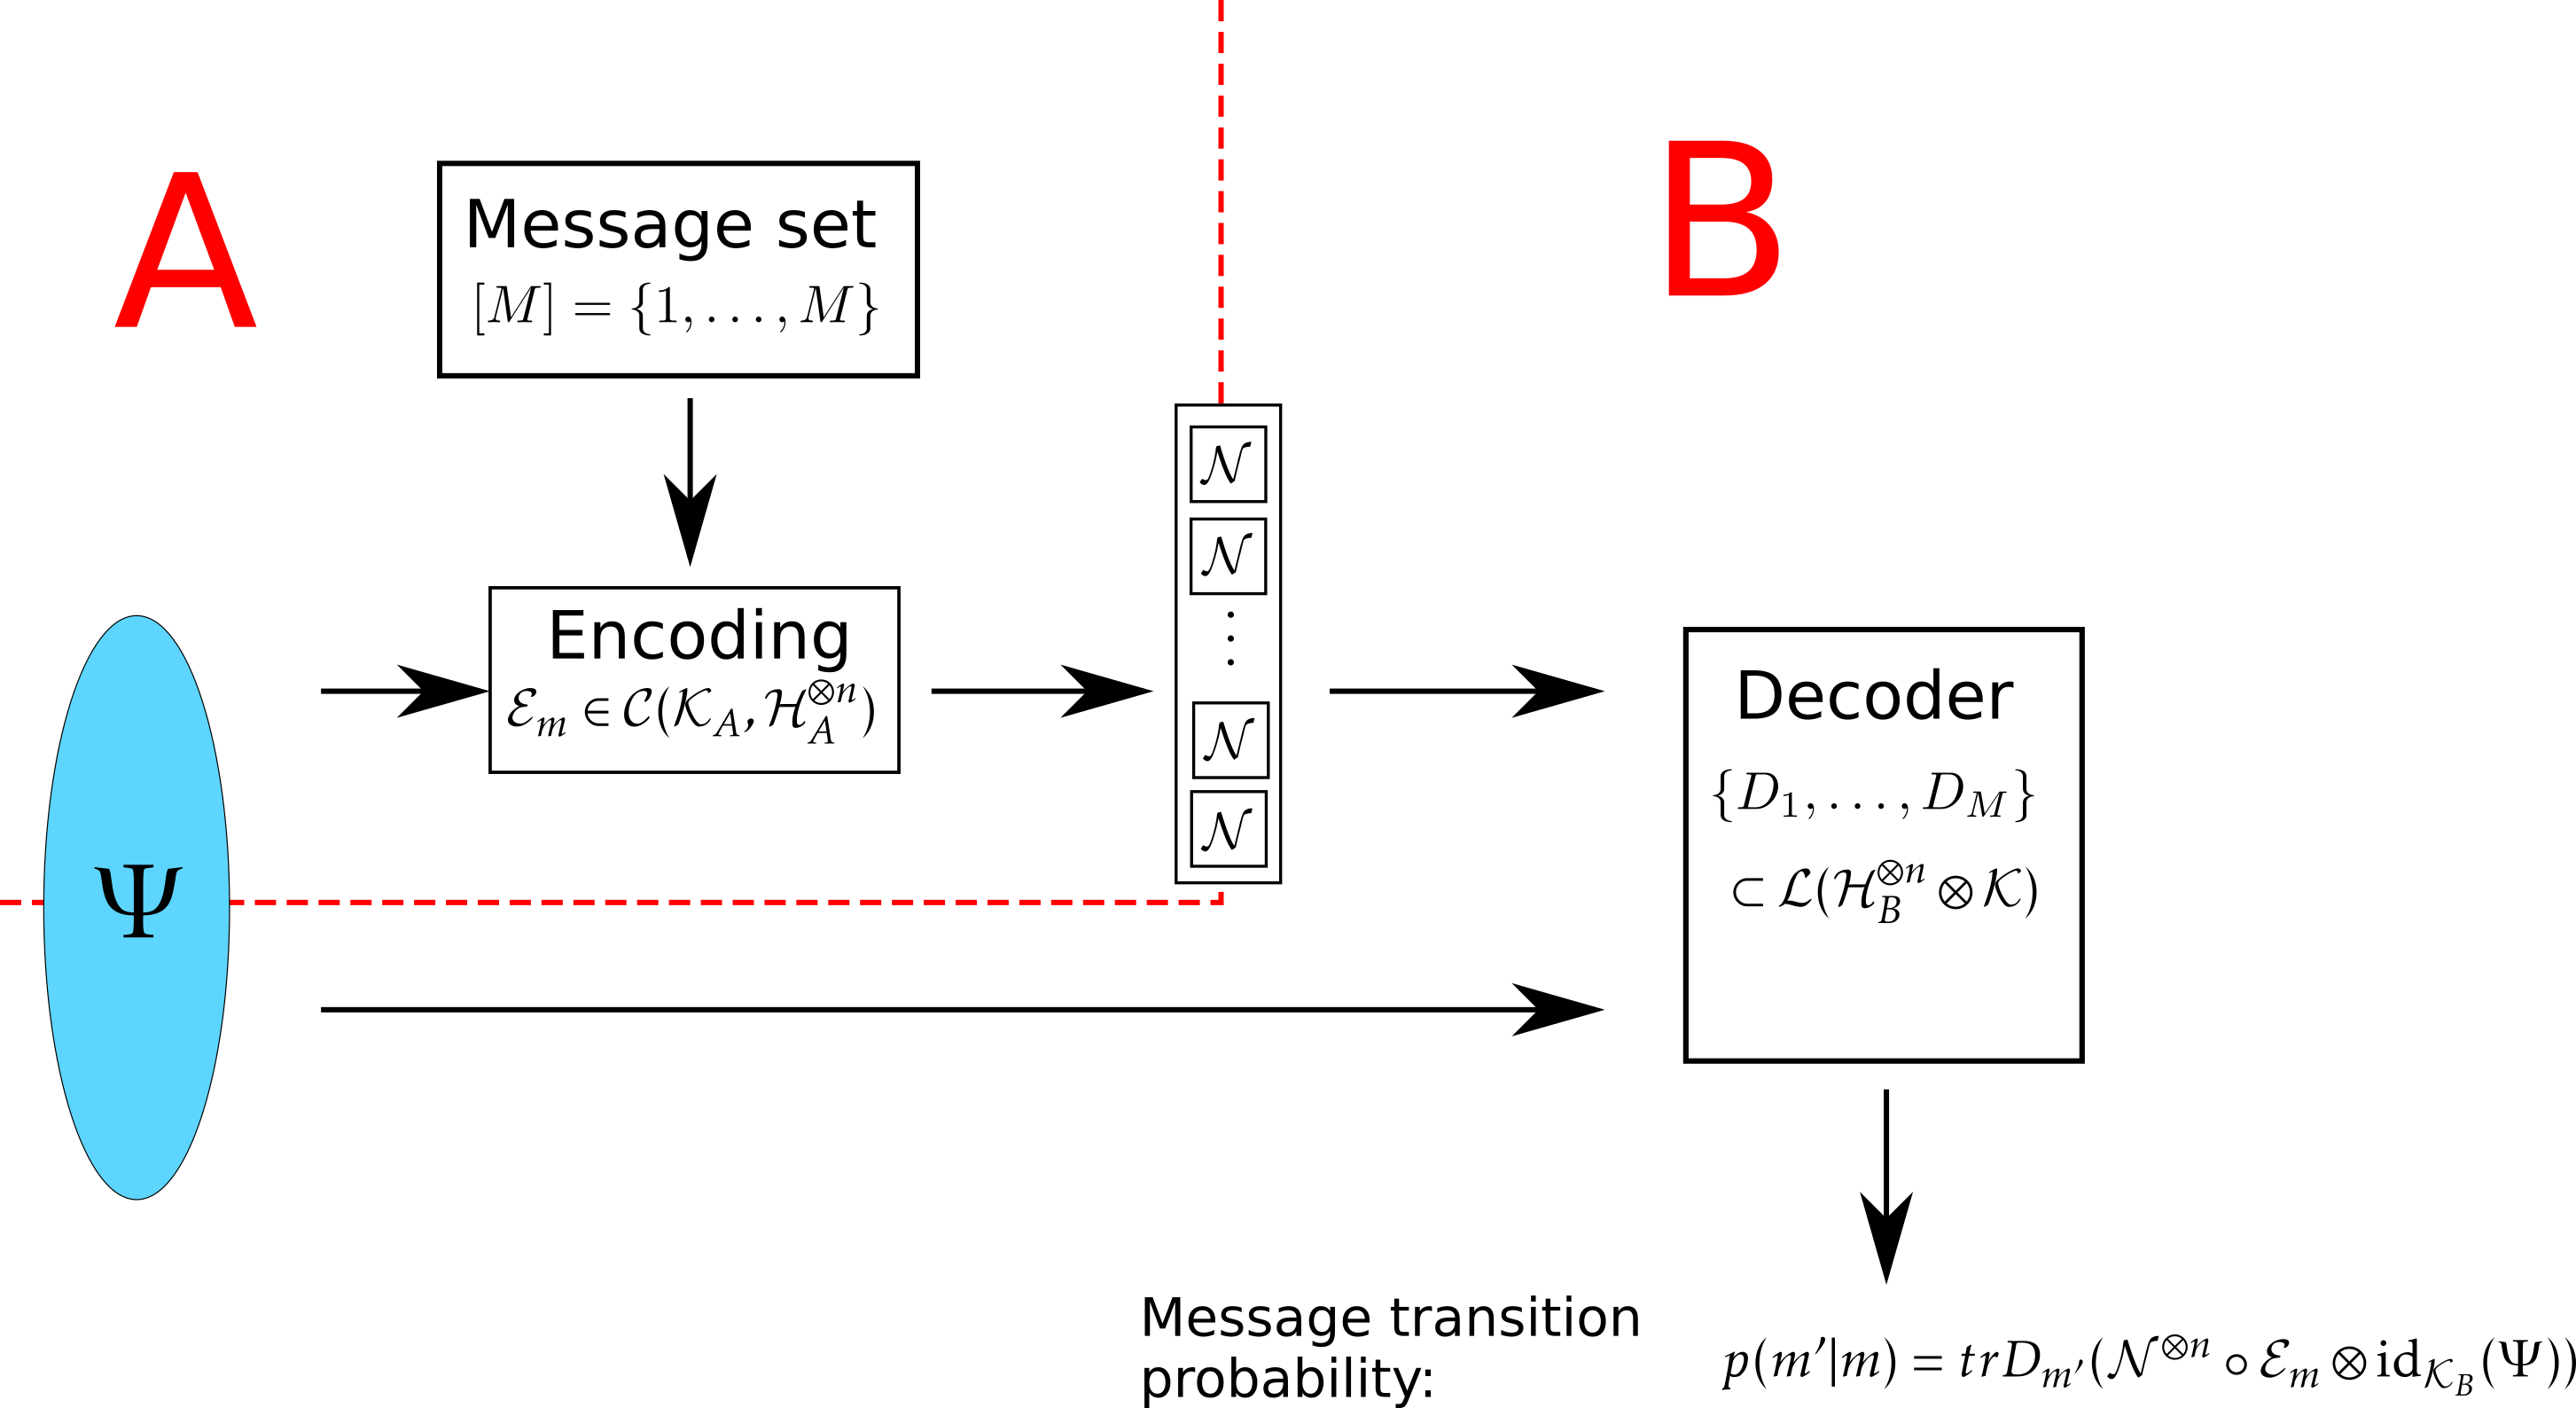
\includegraphics[scale=.8]{pics/entanglement_assisted_coding}
	\vspace{2ex}
\end{center}
We aim to determine the optimal asymptotically achievable message transmission rates in the above scenario. First we give the precise definitions. We fix the abbreviation ``EA'' for ``entanglement-assisted''.
\begin{definition}\label{def:ea_cl_mes_code}
Let $\cN \in \cC(\cH_A \otimes \cH_B)$ be a c.p.t.p. map. An \emph{$(n,M)$-EA message transmission code} for $\cN$ is a family $\cC := (\Psi, \cE_m, D_m)_{m=1}^M$ where
\begin{itemize}
 \item $\Psi := \ket{\psi}\bra{\psi} \in \cS(\cK_A \otimes \cK_B)$ is a pure state shared by sender and receiver. 
 \item $\cE_m \in \cC(\cK_A, \cH_A^{\otimes n})$ is a c.p.t.p. map for each $m \in [M]$, and
 \item $D_m \in \cL(\cH_B^{\otimes n}, \cK_B)$ is a matrix, such that $0 \leq D_m \leq \bbmeins_{\cH_B^{\otimes n} \otimes \cK_B}$, and $\sum_{m=1}^M D_m = \bbmeins_{\cH_B^{\otimes n} \otimes \cK_B}$.
\end{itemize}
\end{definition}
The \emph{average error} of the code $\cC$ is defined by 
\begin{align}
 \overline{e}_{EA}(\cC, \cN^{\otimes n}) \ := \ \frac{1}{M} \sum_{m=1}^M \ \tr D_m^c(\cN^{\otimes n} \circ \cE_m \otimes \id_{\cK_B}(\Psi)),
\end{align}
where we defined, with some abuse of notation $A^c := \bbmeins - A^c$ for each matrix $A$. As we did in case of classical message transmission without entanglement assistance, we define 
\begin{align*}
\overline{N}_{EA}(\cN, n , \epsilon) \ := \ \max\left\{M: \ \exists \ (n,M) \text{- EA message transm. code} \ \cC \ \text{s.t.} \ \overline{e}_{EA}(\cC, \cN^{\otimes n}) \leq \epsilon \right\} 
\end{align*}
for each $\epsilon \in [0,1]$ and $n \in \bbmN$. To state the corresponding capacity theorem, we introduce another quantum entropic quantity. 
\begin{definition}[Quantum mutual information] \index{quantum mutual information}
For a c.p.t.p. map $\cN \in \cC(\cH_A, \cH_B)$ and a state $\rho \in \cS(\cH_A)$, the \emph{quantum mutual information} \index{mutual information!quantum} is defined by
\begin{align}
 I(\rho,\cN) \:= S(\rho) + S(\cN(\rho)) - S(\cN \otimes \id_{\cK}(\ket{\psi}\bra{\psi})), \label{def:qmi_q}
\end{align}
where $\psi$ is the state vector of any purification of $\rho$. 
\end{definition}
\begin{remark}
Notice, that the term on the r.h.s. of Eq (\ref{def:qmi_q}) above is indeed independent of the choice of 
purification.
\end{remark}
\begin{theorem}[Entanglement-assisted capacity]\label{thm:ea_capacity}
Let $\cN \in \cC(\cH_A, \cH_B)$. It holds
\begin{enumerate}
 \item $\forall \epsilon > 0: \ \liminf_{n \rightarrow \infty} \frac{1}{n} \log \overline{N}_{EA}(\cN,n, \epsilon) \ \geq \sup_{\rho \in \cS(\cH_A)} I(\rho, \cN)$, and \label{thm:ea_capacity_1}
 \item $\inf_{\epsilon > 0}: \ \limsup_{n \rightarrow \infty} \frac{1}{n} \log \overline{N}_{EA}(\cN,n, \epsilon) \ \leq \sup_{\rho \in \cS(\cH_A)} I(\rho, \cN)$.  \label{thm:ea_capacity_2}
\end{enumerate}
\end{theorem}
\begin{exercise}
 Convince yourself, that the EA message transmission capacity is the same, when the maximal error criterion is taken into account instead of the average error. 
\end{exercise}
The claims of Theorem \ref{thm:ea_capacity} determine the input-state maximized quantum mutual information as the \emph{entanglement-assisted classical capacity} of the QDMC $\cN$.
Before we prove the claims of the above 
The following proposition states existence of codes sufficient for proving Theorem \ref{thm:ea_capacity}.\ref{thm:ea_capacity_1}. 
\begin{proposition}\label{prop:ea_achiev_codes}
 Let $\cN \in \cC(\cH_A, \cH_B)$ be a c.p.t.p. map, and $\sigma \in \cS(\cH_A)$. For each $\epsilon > 0, \delta > 0$ exists a number $n_0$ such that for each $n > n_0$
 \begin{align*}
  \overline{N}_{EA}(\cN, n ,\epsilon) \ \geq \ \exp\left(n(I(\sigma, \cN) - \delta) \right).
 \end{align*}
\end{proposition}
The strategy to prove the above claim will be, to combine a number of instances of the channel, a given pure bipartite state and certain encoding maps to form an ``effective'' classical-quantum channel. 
Afterwards, it will turn out, that classical message transmission codes for this cq channel can be reformulated to give EA message transmission codes for the original channel again. To support this strategy, we need the following lemma. 
\begin{lemma} \label{lemma:ea_mutual_holevo_approx}
 Let $\cH$ be a Hilbert space, $\dim \cH := d$, $\sigma \in \cS(\cH)$, and 
 \begin{align}
  \psi = \sum_{i=1}^d \sqrt{\alpha_i} v_i \otimes v_i
 \end{align}
 be a Schmidt decomposition of a purification $\psi$ of $\sigma$ ($\alpha_i = 0$ may occur for some $i$), and $k \in \bbmN$. There is a family 
 \begin{align}
  \{\tilde{\cE}_x\}_{x \in \cX} \subset \cC(\cH^{\otimes k}, \cH^{\otimes k}),
 \end{align}
 such that for each Hilbert space $\cK$, and each $\cN \in \cC(\cH, \cK)$ with the cq channel $V: \cX \rightarrow \cS(\cK^{\otimes n} \otimes \cK^{\otimes n})$,
 \begin{align}
  V(x) \ := \ \cN^{\otimes k} \circ \tilde{\cE}_x \otimes \id_{\cH}^{\otimes k}(\ket{\psi}\bra{\psi}^{\otimes k}) &&(x \in \cX)
 \end{align}
 The inequality 
 \begin{align}
  \left|k \cdot I(\rho,\cN) - \chi(q_\ast, V) \right| \ \leq \ 2 d \cdot \log(k+1) \label{lemma:ea_mutual_holevo_approx_1}
 \end{align}
 is fulfilled with $q_\ast$ being the equidistribution on $\cX$.
\end{lemma}
Before proving Lemma \ref{lemma:ea_mutual_holevo_approx}, we recall some properties of the typical sets. 
Let $\cX$ be an alphabet. For each $k \in \bbmN$, we define the set of \emph{$p$-typical words of lengths $k$} by 
\begin{align*}
T_p^k \ := \ \{x^k = (x_1,\dots,x_k): \forall a \in \cX: \frac{1}{k}N(a|x^k) = p(a)\},
\end{align*}
Where $N(a,x^k)$ is the number of occurencies of the letter $a$ in $x^k$. 
It is clear, that for some $p$, $k$, $T_p^k$ is empty. If $T_p^k$ is nonempty, we call 
$p$ a \emph{$k$-type}. We denote the set of all such $k$-types $\cT(\cX,k)$. By elementary counting arguments, it holds 
\begin{align}
|\cT(\cX,k)| \ \leq \ (k+1)^{|\cX|}, \label{type_counting}
\end{align}
i.e. the set of types on a given alphabet does at most increase polynomially with growing blocklengths.
Notice, that 
$
T_\lambda^k \cap T_\mu^k = \emptyset
$
for all $\lambda \neq \mu \in \cT(l,\cX)$. Moreover, 
\begin{align}
\bigcup_{\lambda \in \cT(\cX,k)} T_\lambda^k \ = \ \cX^k. \label{type_collection}
\end{align} 
Summarizing the above relations, we notice that \emph{the collection of sets of typical $k$-words form a disjoint decomposition of} $\cX^k$
The concept of types can be adopted to the quantum setting as follows. Let $\sigma \in \cS(\cH)$ be a given quantum state, and 
\begin{align*}
 \sigma \ = \ \sum_{x \in \cX} \alpha_x \ket{\tau_x}\bra{\tau_x} 
\end{align*} 
be a spectral decomposition of $\sigma$ with an orthonormal basis $\{\tau_x\}_{x \in \cX}$ in $\cH$, $|\cX| = \dim \cH$.
We regard $\alpha$ as a probability distribution on $\cX$ with $\alpha(x) = \alpha_x$. By the properties 
of types and sets of typical words, the collection $\{\cH_\lambda: \lambda \in \cT(\cX,k)\}$ with
\begin{align*}
\cH_\lambda \ := span \{\tau_{x^k} := \tau_{x_1}\otimes \cdots \otimes \tau_{x_k}: \ x^k \in T_\lambda^k\}
\end{align*}
is a collection of mutually orthogonal subspaces of $\cH$ such that $\cH^{\otimes k}$ can be written as a direct sum
of these spaces, i.e. 
\begin{align*}
\cH^{\otimes k} \ = \ \bigoplus_{\lambda \in \cT(\cX, k)} \cH_\lambda.
\end{align*}
Note, that by construction $\dim \cH_\lambda = |T_\lambda^k|$ for each $k$-type $\lambda$. \\
We are now ready for the proof of Lemma \ref{lemma:ea_mutual_holevo_approx}. 
\begin{proof}[Proof of Lemma \ref{lemma:ea_mutual_holevo_approx}]
We fix a blocklength $k$ and abbreviate $\cT_k := \cT(\cX,k)$. Using the Schmidt decomposition of $\psi$
from the hypotheses of the lemma, we write 
\begin{align*}
\psi^{\otimes n} \ 
&= \ \sum_{x^k \in \cX^k} \sqrt{\alpha^k(x^k)} \ \tau_{x^k} \otimes \tau_{x^k} \\
&= \sum_{\lambda \in \cT} \sum_{x^k \in T_\lambda^k} \sqrt{\alpha^k(x^k)} \ \tau_{x^k} \otimes \tau_{x^k}.
\end{align*}
For fixed $k$-type $\lambda$, the $\alpha^k$-probability is constant over the words in $T_\lambda^k$. It 
holds for each $x^k \in T_\lambda^k$
\begin{align*}
\alpha^k(x^k) = \frac{\alpha^k(T_\lambda^k)}{|T_\lambda^k|} =: \frac{\mu_{\lambda}}{|T_\lambda^k|}.
\end{align*}
Therefore, we have with the definition 
\begin{align*}
\phi_\lambda := \frac{1}{\sqrt{|T_\lambda^k|}} \sum_{x^k \in T_\lambda^k} \tau_{x^k} \otimes \tau_{x^k}
\end{align*}
the relations
\begin{align}
\psi^{\otimes k} \
&= \ \sum_{\lambda \in \cT_k} \sum_{x^k \in T_\lambda^k} \sqrt{\alpha^k(x^k)} \ \tau_{x^k} \otimes \tau_{x^k} \nonumber \\
&= \ \sum_{\lambda \in \cT_k} \sqrt{\mu_\lambda}\cdot \frac{1}{\sqrt{|T_\lambda^k|}} \sum_{x^k \in T_\lambda^k} \tau_{x^k} \otimes \tau_{x^k} \nonumber \\
&= \ \sum_{\lambda \in \cT_k} \sqrt{\mu_\lambda}\cdot \phi_\lambda. \label{lemma:ea_mutual_holevo_approx_2}
\end{align}
It is critical to notice here, that for each $k$-type $\lambda$, $\phi_\lambda$ is a maximally entangled state vector on $\cH_\lambda \otimes \cH_\lambda$. For the calculations that follow, we define the shortcuts $d_\lambda := \dim \cH_\lambda$ and $\cY_\lambda := [d_\lambda^2] \times \{0,1\}$ for each $\lambda \in \cT_k$. \newline
Let for each type $\lambda$
\begin{align*}
\{v_{j_\lambda}^{\lambda} \}_{j_\lambda = 1}^{d_\lambda^2} \subset \cL(\cH_\lambda)
\end{align*}
be a family of unitaries as stated in Lemma \ref{lemma:unitary_basis_dense_coding}. We extend each of these to maps on $\cL(\cH^{\otimes n})$ via zero-padding, i.e. 
We define the action of $v_{j_\lambda}^{d_\lambda^2}$ on the orthocomplement of $\cH_\lambda$ by
\begin{align} 
v_{j_\lambda}^{\lambda} x  \ := \ 0 && (x \in \cH_\lambda^\perp)
\end{align}
Define $\cY \ = \ \prod_{\lambda \in \cT} \ \cY_\lambda$ (this is the cartesian product!), 
and for each $\lambda \in \cT_k$, $y_\lambda := (j_\lambda,r_\lambda) \in \cY_\lambda$
\begin{align*}
u_{y_\lambda}^\lambda \:=\ v_{j_\lambda}^\lambda \cdot (-1)^{r_\lambda}.
\end{align*}
We have, using the representation of $\psi^{\otimes k}$ from Eq. (\ref{lemma:ea_mutual_holevo_approx_2}) 
\begin{align}
(u_{y_\lambda}^{\lambda} \otimes \bbmeins^{\otimes k}) \psi^{\otimes k} \ 
= \ \sum_{\gamma \in \cT} \sqrt{\mu_\gamma} (u_{y_\lambda}^{\lambda} \otimes \bbmeins^{\otimes k}) \phi_\gamma  
\ = \ \sqrt{\mu_\lambda}(u_{y_\lambda}^{\lambda} \otimes \bbmeins^{\otimes k}) \phi_\lambda.
\end{align}
The rightmost of the above equalities is by the fact, that $(u_{y_{\lambda}}^\lambda \otimes \bbmeins^{\otimes k})\phi_{\gamma} = \delta_{\gamma \lambda} \phi_\gamma$. We define for each $y = (y_\lambda)_{\lambda \in \cT_k} \in \cY$
\begin{align*}
u_y \ := \ \sum_{\lambda \in \cT_k} u_{y_\lambda}^\lambda, 
\end{align*}
and $\tilde{\cE}_y(a) \ := \ u_y(a)u_y^\ast$ for each $y \in \cY$. Therefore, we have for all $y = (y_\lambda)_{\lambda \in \cT_k}$ 
\begin{align*}
\tilde{\cE_y} \otimes \id_{\cH}^{\otimes k}(\ket{\psi}\bra{\psi}^{\otimes k}) \ 
&= \ \sum_{\lambda, \gamma \in \cT_k} (u_{y_\lambda}^\lambda \otimes \bbmeins^{\otimes k}) \ket{\psi}\bra{\psi}^{\otimes k}(u_{y_\gamma}^\gamma \otimes \bbmeins^{\otimes k})^\ast \\ 
&= \ \sum_{\lambda, \gamma \in \cT_k} (u_{y_\lambda}^\lambda \otimes \bbmeins^{\otimes k}) \ket{\phi_\lambda}\bra{\phi_\gamma}(u_{y_\gamma}^\gamma \otimes \bbmeins^{\otimes k})^\ast. 
\end{align*}
To proceed with the proof we need to show two identities. \\
\begin{align*}
  \text{Identity 1:} \hspace{2cm} \frac{1}{|\cY|} \sum_{y \in \cY} \tilde{\cE}_y \otimes \id_{\cH}^{\otimes k}(\ket{\psi}\bra{\psi}^{\otimes k}) \ = \ \sum_{\lambda \in \cT} \ \mu_\lambda \pi_\lambda \otimes \pi_\lambda,
\end{align*}
where $\pi_\lambda = \frac{\bbmeins_{\cH_\lambda}}{d_\lambda}$ is the maximally mixed state on $\cH_\lambda$ for each type $\lambda$. To prove the above equation, we consider the sum
\begin{align*}
 \frac{1}{|\cY|}\sum_{y \in \cY} (\tilde{\cE}_y \otimes \id_{\cH}^{\otimes k})(\ket{\psi}\bra{\psi}^{\otimes k}) \
 & = \frac{1}{|\cY|}\sum_{y \in \cY}\sum_{\lambda, \gamma \in \cT_k} 
	   \sqrt{\mu_\lambda\cdot \mu_\gamma} (u_{y_\lambda}^\lambda \otimes \bbmeins_{\cH}^{\otimes k})\ket{\psi}\bra{\psi}^{\otimes k}(u_{y_\gamma}^\gamma \otimes \bbmeins_{\cH}^{\otimes k})^\ast \\
 & = \frac{1}{|\cY|}\sum_{y \in \cY}\sum_{\lambda, \gamma \in \cT_k} 
 \sqrt{\mu_\lambda\cdot \mu_\gamma} (u_{y_\lambda}^\lambda \otimes \bbmeins_{\cH}^{\otimes k})\ket{\phi_\lambda}\bra{\phi_\gamma}(u_{y_\gamma}^\gamma \otimes \bbmeins_{\cH}^{\otimes k})^\ast 
 \end{align*}
  We evaluate the inner sums in the last line above for two cases. 
  \begin{itemize}
  	\item $\lambda \neq \gamma$: We have
  	\begin{align*}
     & \sum_{y \in \cY} 
     \sqrt{\mu_\lambda\cdot \mu_\gamma} (u_{y_\lambda}^\lambda \otimes \bbmeins_{\cH}^{\otimes k})\ket{\phi_\lambda}\bra{\phi_\gamma}(u_{y_\gamma}^\gamma \otimes \bbmeins_{\cH}^{\otimes k})^\ast \\
     &= \left(\frac{|\cY|}{|\cY_\lambda|}\right)^2\sum_{y_\lambda \in \cY_\lambda}\sum_{y_\gamma \in \cY_\gamma}
     \sqrt{\mu_\lambda\cdot \mu_\gamma} (u_{y_\lambda}^\lambda \otimes \bbmeins_{\cH}^{\otimes k})\ket{\phi_\lambda}\bra{\phi_\gamma}(u_{y_\gamma}^\gamma \otimes \bbmeins_{\cH}^{\otimes k})^\ast \\
     &= \ \left(\frac{|\cY|}{|\cY_\lambda|}\right)^2 \sum_{r_\lambda, r_\gamma \in \{0,1\}} (-1)^{r_\lambda + r_\gamma} \sum_{j_\lambda \in [d_\lambda^2]} \sum_{j_\gamma \in [d_\gamma^2]}
     \sqrt{\mu_\lambda\cdot \mu_\gamma} (v_{j_\lambda}^\lambda \otimes \bbmeins_{\cH}^{\otimes k})\ket{\phi_\lambda}\bra{\phi_\gamma}(v_{j_\gamma}^\gamma \otimes \bbmeins_{\cH}^{\otimes k})^\ast \\
  	& = \ 0
  	\end{align*} 
  	The last inequality above is by the fact, that $\sum_{r_\lambda, r_\gamma \in \{0,1\}} (-1)^{r_\lambda + r_\gamma}$ vanishes.
    \item $\lambda = \gamma$. In this case, The inner sum reads
    \begin{align*} 
     & \sum_{y \in \cY}
     \mu_\lambda (u_{y_\lambda}^\lambda \otimes \bbmeins_{\cH}^{\otimes k})\ket{\phi_\lambda}\bra{\phi_\lambda}(u_{y_\lambda}^\lambda \otimes \bbmeins_{\cH}^{\otimes k})^\ast  \\
     &= \frac{|\cY|}{|\cY_\lambda|}\sum_{y_\lambda \in \cY_\lambda}
     \mu_\lambda (u_{y_\lambda}^\lambda \otimes \bbmeins_{\cH}^{\otimes k})\ket{\phi_\lambda}\bra{\phi_\lambda}(u_{y_\lambda}^\lambda \otimes \bbmeins_{\cH}^{\otimes k})^\ast  \\
     & = \frac{|\cY|}{|\cY_\lambda|}  \ \sum_{r_\lambda} (-1)^{2 \cdot r_\lambda} \sum_{j_\lambda \in [d_\lambda^2]} 
     \mu_\lambda (v_{j_\lambda}^\lambda \otimes \bbmeins_{\cH}^{\otimes k})\ket{\phi_\lambda}\bra{\phi_\lambda}(v_{j_\lambda}^\lambda \otimes \bbmeins_{\cH}^{\otimes k})^\ast \\
     & = \frac{|\cY|}{|\cY_\lambda|}2 \mu_\lambda \cdot \bbmeins_{\cH}^{\otimes k} \otimes \bbmeins_{\cH}^{\otimes k} \\
     & = \frac{|\cY|}{|\cY_\lambda|}2 d_\lambda^2 \mu_\lambda \pi_\lambda \otimes \pi_\lambda \\
     & = |\cY| \mu_\lambda \pi_\lambda \otimes \pi_\lambda.
    \end{align*} 
  \end{itemize} 
The second identity is
\begin{align*}
    \text{Identity 2:} \hspace{1cm} (\cN \circ \tilde{\cE}_y \otimes \id_{\cH}^{\otimes k})(\ket{\psi}\bra{\psi}^{\otimes k})  \ 
  = \ (\bbmeins^{\otimes k} \otimes u_y^T)\cN \otimes \id_{\cH}^{\otimes k}(\ket{\psi}\bra{\psi}^{\otimes k})(\bbmeins^{\otimes k} \otimes u_y^T)^\ast
\end{align*}
holding for any given c.p.t.p. map $\cN \in \cC(\cH^{\otimes k}, \cK)$ with a Hilbert space $\cK$. To prove Identity 2, we remember the claim of Lemma \ref{lemma:entanglement_trick} from Chapter \ref{chap:source_comp}. If $\phi$ is the state vector of a maximally entangled pure state on $\cF \otimes \cF$, and $A$ a matrix on $\cF$, then
\begin{align*}
(\bbmeins_{\cF} \otimes A)\phi \ = \ (A^T \otimes \bbmeins_{\cF})\phi.
\end{align*}
This fact applied on each $\lambda \in \cT_k$ together with the representation in (\ref{lemma:ea_mutual_holevo_approx_2}) proves the claim. \newline 
From Identity 2 and unitary invariance of the von Neumann entropy, we directly obtain 
\begin{align}
S(\cN \circ \tilde{\cE}_y \otimes \id_{\cH}^{\otimes k}(\ket{\psi}\bra{\psi}^{\otimes k})) \
= \ S(\cN \otimes \id_{\cH}^{\otimes k}(\ket{\psi}\bra{\psi}^{\otimes k}))
\end{align}
Having these equalities, we can calculate
\begin{align*}
S\left(\frac{1}{|\cY|} \sum_{y \in \cY} \cN^{\otimes k} \circ \tilde{\cE}_y \otimes \id_{\cH}^{\otimes k} (\ket{\psi}\bra{\psi}^{\otimes k})\right) \ 
& = \ S\left(\cN^{\otimes k} \otimes \id_{\cH}^{\otimes k}\left(\sum_{\lambda \in \cT} \mu_\lambda \pi_\lambda \otimes \pi_\lambda\right)\right) \\
& \geq  \sum_{\lambda \in \cT_k} \mu_\lambda S(\cN^{\otimes k} \otimes \id_{\cH}^{\otimes k}(\pi_\lambda \otimes \pi_\lambda)) \\
& = \sum_{\lambda \in \cT_\lambda} \mu_\lambda \left( S(\cN^{\otimes k}(\pi_k)) + S(\pi_\lambda)\right)\\
& \geq S\left(\cN^{\otimes k}\left(\sum_{\lambda \in \cT_k} \mu _\lambda \pi_\lambda\right)\right) 
 \ + \ S\left(\sum_{\lambda \in \cT_k} \mu _\lambda \pi_\lambda\right)  
 - 2\ H(\mu) \\ 
& \geq S(\cN(\sigma)^{\otimes k}) \ + \ S(\sigma^{\otimes k}) - d \cdot \log(k+1)
\end{align*}
The first inequality above is by concavity, the second by almost-convexity of the von Neumann entropy (Lemma \ref{lemma:s_almost_convexity}). The last inequality is by our initial representation of $\sigma^{\otimes k}$ in terms of mutually orthogonal projections onto typical subspaces together with the bound $H(\mu) \leq \log |\cT_k| \leq d \cdot \log(k+1)$. \newline 
Choosing $q_\ast$ and $V$ as in the hypotheses of the proposition, we have
\begin{align*}
  \chi(q_\ast, V) \ 
  & = \ S\left(\frac{1}{|\cY|} \sum_{y \in \cY} \cN{\otimes k} \circ \tilde{\cE}_y \otimes \id_{\cH}^{\otimes k} (\ket{\psi}\bra{\psi}^{\otimes k})\right) 
  \ - \ \frac{1}{|\cY|} \sum_{y \in \cY} \ S(\cN^{\otimes k} \circ \tilde{\cE}_y \otimes \id_{\cH}^{\otimes k}(\ket{\psi}\bra{\psi}^{\otimes k})) \\
  & \geq \ S(\cN(\sigma)^{\otimes k}) \ + \ S(\sigma^{\otimes k}) - d \cdot \log(k+1)
    - S(\cN^{\otimes k} \otimes \id_{\cH}^{\otimes k}(\ket{\psi}\bra{\psi}^{\otimes k})) \\
  & = \ k \cdot I(\sigma, \cN) \ - \ d \cdot \log(k+1)
\end{align*}
The reversed inequality can be proven in a similar way.
\end{proof}
Now we are ready to prove Proposition \ref{prop:ea_achiev_codes}. 
\begin{proof}[Proof of Proposition \ref{prop:ea_achiev_codes}]
Set $d_A := \dim \cH_A$, $d_B := \dim \cH_B$, and fix a state $\sigma \in \cS(\cH_A)$. Let
\begin{align*}
\sigma \ = \ \sum_{i=1}^{d_A} \alpha_i \tau_i
\end{align*}
be a spectral decomposition of $\sigma$. Define a pure state $\Psi := \ket{\psi}\bra{\psi} 
\in \cS(\cH_A \otimes \cH_A)$ via
\begin{align*}
\psi := \sum_{i=1}^{d_A} \sqrt{\alpha_i} \tau_i \otimes \tau_i.
\end{align*}
Let $\{\tilde{\cE}\}_{x \in \cX}$ be a family of channels as in Lemma \ref{lemma:ea_mutual_holevo_approx}. Define the cq channel $V: \cX \rightarrow \cS(\cH_B^{\otimes k}\otimes \cH_B^{\otimes k})$ by
\begin{align*}
V(x) \ := \ \cN^{\otimes k} \circ \tilde{\cE}_x \otimes \id_{\cH_B}^{\otimes k}(\Psi^{\otimes k})&& (x \in \cX).
\end{align*}
With Lemma \ref{lemma:ea_mutual_holevo_approx}, we know, that 
\begin{align*}
\chi(q_\ast,V) \ \geq \ k I(\sigma,\cN) - d_A \log(k+1)
\end{align*}
holds. \newline 
Fix $\epsilon, \delta > 0$, and an arbitrary blocklength $n \in \bbmN$. Write $n = a\cdot k + b$ with $a, b \in \bbmN$, $0 \leq b < k$. If $a$ is large enough (which happens for large enough $n$), we have
\begin{align*}
 N(a, V, \epsilon) \ \geq \exp(a (\chi(q_\ast, V)- \frac{\delta}{2})).
\end{align*}
This follows from the achievability statement in Holevo's Theorem. Consequently, there is an $(a,M)$ code $\tilde{\cC} = (u_m, \tilde{D}_m)_{m=1}^M$ for classical message transmission over the DMCQ channel $V$ with 
\begin{align*}
 M \ \geq \ \exp\left(a(\chi(q_\ast, V) -\frac{\delta}{2})\right)
\end{align*}
and average transmission error
$
\overline{e}(\tilde{\cC}, V^{\otimes a}) \ \leq \ \epsilon.
$
We will now use $\tilde{\cC}$ to construct an $(n,M)$ code for entanglement-assisted message transmission over $\cN$. \newline 
Define, for each $m \in [M]$, and each codeword  $u_m = (u_{m,1},\dots, u_{m,a})$ from $\tilde{\cC}$ a c.p.t.p. map $\cE_m \in \cC(\cH_A^{\otimes n} \otimes \cH_A^{\otimes n})$ by
\begin{align*}
\cE_m(\cdot) \ := \ \tilde{\cE}_{u_{m,1}} \otimes \cdots \otimes \cE_{u_{m,a}} \otimes \id_{\cH}^{\otimes b}(\cdot),
\end{align*}
and a POVM $\{D_m\}_{m =1}^M$ on $(\cH_B \otimes \cH_B)^{\otimes n}$ by 
\begin{align*}
D_m \ := \ \tilde{D}_m \otimes \bbmeins_{\cH_B \otimes \cH_B}^{\otimes b}.
\end{align*}
With the preceding definitions, and the pure maximally entangled state $\Psi := \ket{\psi}\bra{\psi}$, $\cC := (\Psi,\cE_m,D_m)_{m=1}^M$ is an $(n,M)$-EA message transmission code for $\cN$. Moreover, it holds for each $m \in [M]$
\begin{align*}
 \tr D_m\left(\cN^{\otimes n} \circ \cE_m(\Psi^{\otimes n})\right) \ 
 & =\ \tr\tilde{D}_m(\bigotimes_{i=1}^a \cN^{\otimes k} \circ \tilde{\cE}_{u_{m,i}} \otimes \id_{\cH_B}^{\otimes k}(\Psi^{\otimes k})) \ \cdot \ \tr(\cN^{\otimes b}\otimes \id_{\cH_B}^{\otimes b}(\Psi^{\otimes b}))\\ 
 & = \tr \tilde{D}_m V^{\otimes a}(u_m).
 \end{align*}
 Arithmetic averaging of the above equality over all messages leads us to
 \begin{align*}
 \overline{e}_{EA}(\cC, \cN^{\otimes n}) \ = \ 1 - \frac{1}{M} \sum_{m=1}^M \tr \tilde{D}_m V^{\otimes a}(u_m) \ \leq \epsilon
 \end{align*}
 Therefore, 
 \begin{align}
 N(n, \cN, \epsilon) \ 
 & \geq \ M \nonumber \\
 &\geq \exp\left(a (\chi(q_\ast,V)-\frac{\delta}{2})\right) \nonumber \\
 &> \exp\left(n \left(\frac{1}{k} \chi(q_\ast,V) - \frac{\delta}{2k} - \frac{1}{kn}(\chi(q_\ast,V)\cdot \frac{\delta}{2k})\right) \right)  \label{fastende}
\end{align}
where the last inequality stems from 
\begin{align*}
a = \frac{n-b}{k} > \frac{n-k}{k} = \frac{n}{k(1 - \frac{1}{n})}.
\end{align*}
Evaluating the exponent on the right hand side of the inequality in (\ref{fastende}), we obtain using Lemma \ref{lemma:ea_mutual_holevo_approx}
\begin{align}
\frac{1}{k} \chi(q_\ast,V) - \frac{\delta}{2k} - \frac{1}{kn}(\chi(q_\ast,V)\cdot \frac{\delta}{2k}) \ 
 & \geq I(\sigma, \cN) - \frac{1}{k}(d_A \log(k+1)) - \frac{\delta}{2} - \frac{1}{n} \chi(q_\ast,V) - \frac{\delta}{2n}. \label{fastfastende}
\end{align}
If $n$ is large enough, we can infer from (\ref{fastende}) and (\ref{fastfastende}), that the claimed 
inequality 
\begin{align*}
\overline{N}_{EA}(n,\cN, \epsilon) \ \geq \ \exp(n(I(\sigma,\cN)- \delta))
\end{align*}
is fulfilled.
\end{proof}

\begin{lemma} \label{lemma:ent_ass_conv_pre}
	Let $\cN \in \cC(\cH_A, \cH_B)$, $\Psi \in \cS(\cH_A \otimes \cK_B)$ be a pure state, $\{\cE_m\}_{m=1}^{M} \subset \cC(\cH_A, \cH_A)$, and $q \in \cP([M])$. Define the c.p.t.p. map $\cE(\cdot) := \sum_{m\in [M]} q(m) \cE_m(\cdot)$, and $\rho_A \:= \ \tr_{\cK_B}\Psi$. With the cq channel $V:\ [M] \rightarrow \cS(\cH_B \otimes \cK_B)$,
	\begin{align*}
	 m \ \mapsto \ V(m) \ := \ \cN\circ \cE_m \otimes \id_{\cK_B}(\Psi),
	\end{align*}
	it holds 
	\begin{align}
	\chi(q,V) \ \leq \ I(\cE(\rho_A), \cN).  
	\end{align}
\end{lemma}
\begin{proof}
We introduce the shortcuts 
\begin{align*}
\tilde{\rho}_m \ := \ \cE_m \otimes \id_{\cK_B}(\Psi), \hspace{.5cm} \text{and} \hspace{.5cm} \rho_{B} \ := \ \tr_{\cK_A \Psi}
\end{align*}
for each $m \in [M]$. By subadditivity of the von Neumann entropy, we have 
\begin{align*}
\chi(q,V) \
&= \ S\left(\cN\circ \cE \otimes \id_{\cK_B}(\Psi)\right) 
 - \sum_{m=1}^M q(m) \ S(\cN \otimes \id_{\cK_B}(\tilde{\rho}_m)) \\
&\leq S\left(\cN\circ \cE(\rho_{A}) \right)   + S(\rho_B) -  \sum_{m=1}^M q(m) \ S(\cN \otimes \id_{\cK_B}(\tilde{\rho}_m)) 
\end{align*}
We aim to further bound the expression
\begin{align}
 \sum_{m=1}^M q(m) \left( S(\rho_B) - S(\cN \otimes \id_{\cK_B}(\tilde{\rho}_m))\right).
\end{align}
 To this reason, we first derive an estimate for each of the summands on the r.h.s. of the above inequality.
 Let, with a suitable additional Hilbert space $\cH_R$, for each $m \in [M]$ $\Gamma_m \in \cS(\cH_A \otimes \cH_R)$ be a purification or $\tilde{\rho}_{A,m}$. We show the inequality
 \begin{align}
 S(\rho_B) - S(\cN\otimes \id_{\cK_B}(\tilde{\rho}_m)) \ \leq \ S(\tilde{\rho}_{A,m}) - S(\cN \otimes \id_{\cH_R}(\Gamma_m)). \label{lemma:ent_ass_conv_pre_1}
 \end{align}
 Let $u_m: \cH_A \rightarrow \cH_B \otimes \cH_E$ be a Stinespring isometry for $\cE_m$, and $\cU_m(\cdot) := u_m(\cdot)u_m^\ast$ the corresponding unitary transformation. Observe, that $\cU_m \otimes \id_{\cK_B}(\Psi)$ is a purification of $\tilde{\rho}_{A,m}$. Consequently 
 \begin{align*}
 S\left((\cN \otimes \id_{\cH_E \otimes \cK_B})\circ(\cU_m \otimes \id_{\cK_B})\Psi \right)
 \ = \ S((\cN \otimes \id_{\cH_R})(\Gamma_m))
 \end{align*}
 holds. Moreover, 
 \begin{align*}
 S(\tilde{\rho}_{A,m}) \ = \ S(\tr_{\cH_A}\Gamma_m) \ = \ S(\tr_{\cH_A}(\cU_m \otimes \id_{\cH_B})(\Psi))
 \end{align*}
 The rightmost inequality above holds, because $\Gamma_m$ and $\cU \otimes \id_{\cH_B}(\Psi)$ are both purifications of $\tilde{\rho}_{A,m}$. For the calculations to come, we use the state 
 \begin{align*}
	\sigma_{m} \ 
	&:= \ (\cN \otimes \id_{\cK_B \otimes \cH_E})\circ (\cU_m \otimes \id_{\cK_B})(\Psi)
	%\sigma_{B'B,m} \
	%&:= \ \tr_{\cH_E} \sigma_{B'BE} \sigma_{B'BE} \ = \cN \otimes \id_{\cK_B}(\tilde{\rho}_m) \\
 \end{align*}
  It then holds
  \begin{align*}
  S(\rho_B) - S(\cN \otimes \id_{\cK_B}(\tilde{\rho}_m)) \ 
  &= \ S(\sigma_{B,m}) - S(\sigma_{BB',m}) \\
  &= \ -S(B'|B, \sigma_{BB'E,m}) \\
  &\leq \ -S(B'|BE, \sigma_{BB'E,m}) \\ 
  &= \ S(\sigma_{BE,m}) - S(\sigma_{BB'E,m}) \\
  &= \ S(\tr_{\cH_A} \Gamma_m) - S(\cN \otimes id(\Gamma_m)). 
  \end{align*}
  Therefore, (\ref{lemma:ent_ass_conv_pre_1}) is valid. We will now show, that the function
  $f: \cS(\cH_A) \ \rightarrow \bbmR$,
  \begin{align*}
    f(\tau) \ := \ S(\tau) - S(\cN \otimes \id_{\cH_R}(\Phi))
  \end{align*}
   is concave. Introduce the isometric channel $\cV(\cdot) := v(\cdot)v^\ast$ where 
   $v: \cH_A \rightarrow \cH_B \otimes \cH_E$ is a Stinespring isometry for $\cN$ with a 
   suitable additional Hilbert space $\cH_E$. Define
   \begin{align*}
	\tilde{\Phi} \ := \ \cV \otimes \id_{\cH_R}(\Phi).
   \end{align*}
   (notice, that the state defined is pure). Denote the marginals of $\tilde{\Phi}$ on the respective subsystems by
   $\gamma_A, \gamma_{BE}$, $\gamma_{BR}$. It holds
   \begin{align*}
   S(\tau) = S(\gamma_{BE}), \hspace{.5cm} S(\gamma_{BR}) = S(\gamma_E). 
   \end{align*}
   Therfore 
   \begin{align*}
       f(\tau) \ = \ S(\tau) - S(\cN \otimes \id_{\cH_R}(\Phi)) \ 
       &= \ S(\gamma_{BE}) - S(\gamma_E) \\
       &= \ S(B|E,\gamma_{BE}) \\
       &= \ S(B|E, \cV(\tau))
   \end{align*}
	Since the map $\tau \mapsto \cV(\tau)$ is affine, and the conditional von Neumann entropy is concave, $f$ is indeed a concave function.
    Putting everything together, we have 
  \begin{align*}
  \chi(q,V) \
  %&= \ S\left(\sum_{m=1}^M q(m) \cN \otimes \id_{\cK_B}(\tilde{\rho}_m)\right) \ - \ \sum_{m=1}^M q(m) S(\cN \otimes \id_{\cK_B}(\tilde{\rho}_m)) \\
  &\leq \ S(\cE(\rho_A)) +  \sum_{m=1}^M q(m) \left( S(\rho_B) - S(\cN \otimes \id_{\cK_B}(\tilde{\rho}_m))\right) \\
  &\leq \ S(\cE(\rho_A)) +  \sum_{m=1}^M q(m) \left( S(\tr_{\cH_A} \Gamma_m) - S(\cN \otimes \id_{\cK_B}(\Gamma_m))\right) \\
  &=  \ S(\cE(\rho_A)) + \sum_{m=1}^M q(m) f(\tilde{\rho}_{A,m}) \\
  &\leq \ S(\cE(\rho_A)) + f(\cE(\rho_A)) \\
  &\leq \ I\left(S(\cE(\rho_A)), \cN \right).
  \end{align*}
\end{proof}
We are now equipped with the prerequisites necessary to prove Theorem \ref{thm:ea_capacity}.
\begin{proof}[Proof of Theorem \ref{thm:ea_capacity}]
	The achievability part (Theorem \ref{thm:ea_capacity}.\ref{thm:ea_capacity_1}) follows indeed from Proposition \ref{prop:ea_achiev_codes} via executing the lower limit. To prove the converse (Theorem \ref{thm:ea_capacity}.\ref{thm:ea_capacity_2}), fix an arbitrary blocklength $n$ and let $\cC \ := \ (\Phi, \cE_m, D_m)_{m=1}^M$
	be an $(n,M)$-EA message transmission code with
	\begin{align*}
	\overline{e} \ := \ \overline{e}_{EA}(\cC,\cN^{\otimes n}) \ < \ 1.
	\end{align*}
	We define states 
	\begin{align}
	\rho \:= \ \tr_{\cK_B} \Phi, \hspace{.3cm} \text{and} \hspace{.5cm} \overline{\tau} := \sum_{m=1}^M 
	p_{\ast}(m) \cE_m(\rho).
	\end{align}
	where $p_\ast$ denotes the equidistribution on the message set, i.e. 
	$
	p_{\ast}(m) \ = \ \frac{1}{M} 
	$
	for each $m$. We define $\overline{\tau}_i$ as the marginal state deriving from $\overline{\tau}$ on the $i$th tensor factor of $\cH^{\otimes n}$. 
	By subadditivity of the quantum mutual information, it holds
	\begin{align}
	I(\overline{\tau}, \cN^{\otimes n}) \ \leq \ \sum_{i=1}^n \ I(\overline{\tau}_i, \cN).
	\label{ent_ass_conv_subadd_used}
	\end{align}
	Define a cq channel $V: \ [M] \rightarrow \cS(\cH_B^{\otimes n} \otimes \cK_B)$ by
	\begin{align*}
	V(m) \ := (\cN^{\otimes n}\circ \cE_m \otimes \id_{\cK_B})(\Phi).
	\end{align*}
	Let $X$ be a random variable with values in $[M]$ and 
	\begin{align}
	\Pr\left(X =m \right) \ = \ \frac{1}{M} \ = \ p_\ast(m),
	\end{align}
	and conditional probabilities 
	\begin{align*}
	\Pr\left(Y = m'|X = m \right) \ := \ \tr D_{m'} V(m) &&(m,m' \in [M])
	\end{align*}
	Then
	\begin{align*}
	\Pr\left(X \neq Y\right) \ = \ \overline{e}_{EA} := \overline{e}.
	\end{align*}
	Using the above inequality and Fano's Lemma, we have
	\begin{align}
	H(X|Y) \ 
	& \ \leq \Pr\left(X \neq Y\right) \log M + h(\Pr(X \neq Y))  \nonumber \\
	& \ = \overline{e} \log M + h(\overline{e}) \nonumber \\
	& \ \leq \overline{e} \log M + 1. \label{ent_ass_conv_fano_use}
	\end{align}
	Moreover, the following chain of (in)equalities is valid. 
	\begin{align}
    \chi(p_\ast,V) \ 
	\leq \ I(\overline{\tau}, \cN^{\otimes n}) \ 
	\leq \sum_{i=1}^n I(\overline{\tau}_i, \cN) \
	\leq n \cdot I\left(\frac{1}{n}\sum_{i=1}^n \overline{\tau}_i, \cN\right) 
    \leq n \underset{\rho \in \cS(\cH_A)}{\sup} I(\rho,\cN). \label{ent_ass_conv_fastende}
	\end{align}
	The first of the above inequalities is justified by Lemma \ref{lemma:ent_ass_conv_pre}, and the definition of $\overline{\tau}$. The second 
	is Eq. (\ref{ent_ass_conv_subadd_used}). The third is by concavity of the quantum mutual information in the first argument. It consequently holds 
	\begin{align*}
	\log M \
	& = \ H(X)  \\
	& = \ I(X;Y) + H(X|Y) \\ 
	& \leq \ I(X;Y) + \overline{e} \log M + 1 \\ 
	& \leq \ \chi(p_\ast,V) + \overline{e} \log M + 1 \\ 
	& \leq n \underset{\rho \in \cS(\cH_A)}{\sup} I(\rho,\cN) + \overline{e} \log M + 1.
	\end{align*}
	The first inequality above is (\ref{ent_ass_conv_fano_use}). The second is by Holevo's bound, and the third is (\ref{ent_ass_conv_fastende}).
	Since $\cC$ was arbitrary, 
	\begin{align}
	 \frac{1}{n} \log \overline{N}_{EA}(n, \cN, \overline{e}) \ \leq \ \underset{\rho \in \cS(\cH_A)}{\sup} I(\rho, \cN) + \frac{\overline{e} \log M}{n} + \frac{1}{n}.
	\end{align}
	Taking limits on both sides of the above inequality proves the converse.
	\end{proof}




\part{Supplements}
\chapter*{Mathematical preliminaries and notation}
\label{chap:preliminaries}
In this lecture we review some basic mathematical definitions which may in most parts be taught in usual higher math courses. At the same time we fix the notation for the forthcoming lectures, and get used to the so-called Dirac notation common in quantum (information) theory. 

\begin{section}{Linear algebra}
The mathematical playground for quantum theory are \emph{Hilbert spaces} \index{Hilbert space} (i.e. a linear space with a scalar product, which is closed in the norm deriving from the
scalar product.) For this course, we will assume, that each Hilbert space is a finite dimensional euclidean space over the field of complex numbers. Under this restriction, the terminology ``Hilbert space'' 
is rather superfluous. However, it is standard in the quantum information theory literature also for finite dimensions, therefore, we keep it. \newline 
If we fix a basis for an Hilbert space $\cH$,  $d:= \dim \cH < \infty$, $\cH$ is isomorph to $\bbmC^d$, where each vector $v \in \cH$ corresponds to a column vector 
\begin{align}
  v = \left(\begin{array}{c} v_1 \\ \vdots  \\ v_d \end{array}\right) 
\end{align}
with entries $v_1,\dots, v_d \in \bbmC$. We use the standard euclidean scalar product $\braket{\cdot,\cdot}: \cH \times \cH \ \rightarrow \bbmC$ defined by
\begin{align}
 \braket{v,w} \ := \ \sum_{i=1}^d \overline{v}_i w_i  
\end{align}
for each $v = (v_1,\dots,v_d), \ w = (w_1,\dots,w_d) \ \in \bbmC^d$ (where $\overline{v}$ is the notation for the complex conjugate of $v$.) \\
We will freely switch between the abstract and component notation, i.e. assuming that an orthonormal basis is fixed, we will not distinguish between a $d$-dimensional Hilbert space 
$\cH$ and $\bbmC^d$. If not otherwise stated, we assume the basis to be the canonical orthonormal basis $\{e_i\}_{i=1}^d$ where 
\begin{align}
  e_i := \left(\begin{array}{c} 0 \\ \vdots \\ 1 \\  \vdots \\ 0 \end{array}\right)
\end{align}
with the $i$-th entry being $1$ and all other entries being $0$. With two Hilbert spaces $\cH$, and $\cH'$ we denote the set of linear maps from $\cH$ to $\cH'$ by $\cL(\cH,\cH')$. 
If we fix a bases in the underlying spaces $\cH$, $\cH'$, $\cL(\cH,\cH')$ is isomorphic to the set
%\begin{align}
 $\bbmM_{d \times d'}(\bbmC)$
%\end{align}
of $d \times d'$ matrices with complex entries, sometimes, we will also write a matrix $A$ as the collection of its entries. $A = (a_{ij})_{i=1,j=1}^{m,n}$ then corresponds to the matrix 
\begin{align}
 A := \left( \begin{array}{ccc} a_{11} & \cdots & a_{1n} \\ \vdots & \ddots & \vdots \\ a_{m1} & \cdots & a_{mn} \end{array} \right) 
\end{align}
If $\cH'$ equals $\cH$, we will also use the shortcut $\cL(\cH)$ for the set $\cL(\cH,\cH')$. We denote the \emph{adjoint matrix} to $A$ by $A^\ast$, the \emph{transposed matrix} to $A$ by $A^T$, i.e. 
\begin{align}
 A^\ast := \left( \begin{array}{ccc} \overline{a}_{11} & \cdots & \overline{a}_{m1} \\ \vdots & \ddots & \vdots \\ \overline{a}_{1n} & \cdots & \overline{a}_{nm} \end{array} \right) \hspace{.5cm} \text{and} \hspace{.5cm}
 A^T := \left( \begin{array}{ccc} a_{11} & \cdots & a_{m1} \\ \vdots & \ddots & \vdots \\ a_{1n} & \cdots & a_{nm} \end{array} \right).
\end{align}
The reader should note, that the transposition is dependent on the chosen basis, while the adjoint is not. The \emph{trace} of a square matrix $A \in \cL(\cH)$ is defined by
\begin{align}
 \tr(A) := \sum_{v_i, A v_i},
\end{align}
where $\{v_1,\dots, v_{\dim_{\cH}}\}$ is an orthonormalbasis in $\cH$. Using the trace, we can define the \emph{Hilbert-Schmidt scalar product} on $\cL(\cH)$, 
\begin{align}
 \braket{A,B}_{HS} \ := \ \tr(A^\ast B) &&(A,B \in \cL(\cH)).
\end{align}
By the (finite dimensional) Riesz representation theorem, there is a one-to-one relationship between $\cH$ and its dual space $\cH^\ast$, i.e. to each 
linear functional $f \in \cH^\ast$ there is a unique element $v_f \in \cH$, such that 
\begin{align}
 f(w) := \braket{v_f, w} 
\end{align}
for each $w \in \cH$. This fact is reflected by the so-called \textbf{Dirac notation}\index{Dirac notation}. In this notation, each element $v \in \cH$ is written as a ``ket'' \index{``ket''} $\ket{v}$, while the
corresponding element $v^\ast \in \cH^\ast$ with 
\begin{align}
  v^\ast(w) = \braket{v,w} 
\end{align}
for each $w \in \cH$ is written as a ``bra'' \index{``bra''} $\bra{v}$. Note, that $\bra{\alpha \cdot v} = \overline{\alpha} \bra{v}$ for all $\alpha \in \bbmC$. Moreover, $\bra{v_1 + v_2} = \bra{v_1} + \bra{v_2}$. 
The \emph{outer product} \index{product!outer} of $w \in \cH,   \in \cH'$, $\ket{v}\bra{w} \in \cL(\cH, \cH')$ is the rank one matrix with the property, 
that 
\begin{align}
  (\ket{v}\bra{w})\ket{x} = \braket{w,x} \ket{v}
\end{align}
holds for all for all $x \in \cH$. It holds $(\ket{v}\bra{w})^\ast = \bra{w}\ket{v}$. The canonical basis in $\cL(\cH, \cH')$ is given by the \emph{matrix units} \index{matrix!unit} $\{E_{ij}\}_{i=1,j=1}^{\dim \cH, \cH'}$, where $E_{ij}$ is the matrix with the $i,j$-entry being
one and all others being zero. 
The following subsets of $\cL(\cH)$ will be of some importance for our considerations. 
\begin{align*}
 \cL^h(\cH) &:= \{A \in \cL(\cH): \ A^\ast = A  \}   					&\text{(Hermitian maps)} \\ 
 \cL^+(\cH) &:= \{A \in \cL(\cH): \ \forall x \in \cH: \ \braket{x,Ax} \geq 0\}	&\text{(positive semidefinite maps)} 
\end{align*}
\index{map!positive semidefinite} We call a map $p \in \cL(\cH)$ an \emph{(orthogonal) projection} \index{projector}, if it is hermitian and idempotent, i.e. $p = p p = p^2$.  \\
 We call a number $\lambda \in \bbmC$ an eigenvalue \index{eigenvalue} of $A \in \bbmM_n$, if there exists $x \in \bbmC^n$, $x \neq 0$, such that $Ax = \lambda x$ (in wich case $x$ is called
 an eigenvector for $A$ to eigenvalue $\lambda$, equivalently, $\lambda$ is an eigenvalue. 
  We denote the spectrum of $A$ (the set of eigenvalues) by $\spec(A)$. 
We say two maps $A,B \in \bbmM_n$ commute, if their commutator \index{commutator}, i.e. the function
\begin{align}
 [A,B] := AB -BA 
\end{align}
vanishes. A very important consequence of being hermitian is existence of an orthonormal basis of eigenvectors, i.e. a spectral decomposition. 
\begin{theorem}[Spectral decomposition] \index{decomposition!spectral}
 Let $A \in \cL(\cH)$ be normal. Then there exists an orthonormal basis $\{v_i: \ 1 \leq i \leq \dim \cH \}$, such that 
 \begin{align}
  \sum_{i = 1}^{\dim \cH} \alpha_i \ket{v_i}\bra{v_i}
 \end{align}
 holds. The numbers $\alpha_1,\cdots, \alpha_{\dim \cH}$ are the eigenvalues of $A$ (counted with multiplicities).
 \end{theorem}
 If $A \in \cL^h(\cH)$, then all eigenvalues are real numbers. 
 \begin{theorem}[Singular value decomposition] \label{thm:svd}
 Let $A \in \cL(\cH, \cK)$. Then there exist orthonormal systems $\{\varphi\}_{i=1}^r \subset \cH$ and $\{\psi\}_{j=1}^r \subset \cK$ such that 
 \begin{align}
   A = \sum_{i,j=1}^r \sigma_j(A) \ket{\varphi_i}\bra{\psi_j}
 \end{align}
 holds, where $r$ is the rank of $A$ and $\sigma_1(A) \geq \dots \geq \sigma_r(A) > 0$ are the singular values (i.e. the eigenvalues of the positive semidefinite matrix $A^\ast A$.)
 \end{theorem}
  The spectral theorem allows to exted real functions in a natural way to hermitian matrices. Let $\cW \subset \bbmR$, and
 $f: \cW \rightarrow \bbmR$. We define for each hermitian map $A \in \cL(\cH)$ with $\spec(A) \subset \cW$
 \begin{align}
  f(A) := \sum_{i=1}^{\dim \cH} f(\alpha_i) \ket{v_i} \bra{v_i},
 \end{align}
 using a spectral decomposition $A := \sum_{i = 1}^{\dim \cH} \alpha_i \ket{v_i} \bra{v_i}$. Particular examples of such matrix-functions we consider in this lecture are 
 the square-root, the exponential functions and logarithms.
 \begin{remark}
  Using matrix functions one has to be very cautious when applying properties of the real functions in the matrix setting. E.g. the identities
  \begin{align}
   \sqrt{AB} = \sqrt{A}\sqrt{B}, \ \text{and} \ \exp{A+B} = \exp{A}\exp{B} 
  \end{align}
  do not hold in general. We also can define a matrix version of the absolute value of a complex number. 
  \begin{theorem}[Polar decomposition] \index{decomposition!polar}
  Let $A \in \cL(\cH,\cK)$. We can write $A$ in the form 
  \begin{align}
   A := |A|U 
  \end{align} 
  where $|A| := \sqrt{A^\ast A}$, and $U$ is a (partial) isometry.
 \end{theorem}
 \end{remark}
 Important norms on $\cL(\cH, \cH')$ are 
 \begin{align}
  \|A\|_1 &:= \tr \sqrt{A^\ast A} & \text{(trace norm)} \\
  \|A\|_2 &:= \sqrt{\tr A^\ast A} = \sqrt{\braket{A,A}_{HS}} & \text{(Hilbert-Schmidt norm)}
 \end{align} \index{trace norm} \index{Hilbert-Schmidt norm}
 We will sometimes identify $\bbmC^n$ with $\bbmR^{2n}$ using the isomorphism 
 \begin{align}
  z \mapsto \left(\begin{array}{c} Re(z) \\ Im(z) \end{array}\right)
 \end{align}
 For fixed Hilbert space $\cH$, we equip the set $\cL^+(\cH)$ with a semiorder \footnote{A semiorder is distinguished from an order by lacking the trichotomy property, i.e. not all pairs of elements can be compared} trace $\geq$. We define for each two matrices $A,B \in \cL(\cH)$
 \begin{align}
  A \ \geq \ B \ :\Leftrightarrow A-B \ \text{positive semidefinite}.
 \end{align}
 The above definition also motivates to write $A \geq 0$ to indicate that $A$ is positive semidefinite. We have 
 \begin{lemma}[Conjugation rule] \label{lemma:conjugation_rule}
   Let $A,B$ be hermitian matrices, $C$ a matrix. It holds 
   \begin{align*}
    A \leq B \ \Rightarrow \ CAC^\ast \leq CBC^\ast.
   \end{align*}
  \end{lemma}
 \end{section}
 
 \begin{section}{Finite-valued random variables and random matrices}
  The usual way, to establish events on a set $\Omega$ is to specify a \emph{$\sigma$-Algebra}. This is a family $\Sigma$ of subsets of $\Omega$ which has the following properties
  \begin{itemize} 
   \item $\emptyset,  \Omega \in \Sigma$, 
   \item If $A, B \in \Sigma$, then $A \cap B \in \Sigma$, and 
   \item If $A_1,A_2,\dots \in \Sigma$, $\bigcup_{i=1}^\infty \in \Sigma$.
  \end{itemize}
  A \emph{probability measure} is then a $\sigma$-additive set function, i.e. a function $\mu: \Sigma \rightarrow \bbmR$ such that 
  \begin{itemize}
   \item $\mu(\emptyset) = 0$ and $\mu(\Omega) = 1$, 
   \item For each family $\{A_i\}_{i=1}^\infty \subset \Sigma$, $A_i \cap A_j = \emptyset$ $i \neq j$, $\mu(\bigcap_{i=1}^\infty A_i) = \sum_{i=1}^\infty \mu(A_i)$. 
  \end{itemize}
  The pair $(\Omega,\Sigma)$ is called a measureable space, the triple $(\Omega, \Sigma, \mu)$ is then called a \emph{probability space}. Let $(\Omega, \Sigma)$, $(\Omega', \Sigma')$ 
  be two measurable spaces. A \emph{random variable} is a map $X: \Omega \rightarrow \Omega'$, such that $X^{-1}(A) \in \Sigma$ for each $A \in \Sigma'$. For each set $\Omega$, the power 
  set forms a $\sigma$-algebra. If the set is not countable, however, the power set may be ``too large to be useful''. A standard $\sigma$-algebra for $\bbmR$ is the so-called \emph{Borel $\sigma$-algebra}, 
  which is the smallest $\sigma$-algebra containing all open sets in $\bbmR$. 
  All random quantities in this course will be assumed to have only a finite range of possible values, i.e. we assume $\Omega$ to be a finite set and implicitely work with the $\sigma$-algebra formed by the 
  members of the power set. \\
  Therefore, we will restrain from introducing the full measure-theoretic framework for probability. 
  Instead introducing sigma algebras and measures on the formal levels, we note, that each probability law or ``probability distribution'' is uniquely determined by the values on the atomic sets. We therefore
  define a probability distribution on a finite set $\cX$ to be function $p: \cX \rightarrow [0,1]$ such that $\sum_{x \in \cX} p(x) = 1$. The probability, that a random variable with distribution (or law) $p$ 
  takes a value in a set $A \subset \cX$ is 
  \begin{align}
   \prob(X \in A) = \sum_{x \in A} p(x).
  \end{align}
  The expectation of $X$ is defined by 
  \begin{align}
   \bbmE X = \sum_{x \in \cX} p(x) x.
  \end{align}
   \begin{proposition}[Law of large numbers]
    Let $X_1,X_2,\dots$ be an i.i.d. sequence of real random variables, $\delta > 0$. It holds
    \begin{align}
     \lim_{N \rightarrow \infty} \prob\left(\left| \frac{1}{N} \sum_{i=1}^N X_i - \bbmE X\right | \geq \delta \right) = 0. 
    \end{align}
   \end{proposition}
 \end{section}

 \begin{section}{Convex analysis} 
A set $A \subset \bbmR^n$ is called \emph{convex} \index{set!convex} \index{convex!set}, if for each elements $x_1,\dots, x_N \in A$ and real numbers $\lambda_1,\dots \lambda_N \in [0,1]$
 such that $\sum_{i=1}^N \lambda_i = 1$, the \emph{convex combination} \index{convex combination} 
 \begin{align}
  x = \sum_{i=1}^N \lambda_i x_i 
 \end{align}
 is also an element of $A$ (i.e. ``A is closed under forming finite convex combinations''). An element $x$ of a convex set $X \in \bbmR^n$ is called \emph{extremal}, if all convex combinations representing $x$ are trivial, i.e. if
 for all $b_1, b_2 \in X$, $\lambda \in [0,1]$ either $b_1 = b_2 = x$ or $\lambda \in \{0,1\}$ holds. Let $A \subset \bbmR^d$ be a convex set. A function $f: A \rightarrow \bbmR$
 is called \emph{convex} \index{convex!function} \index{function!convex}, if  
 \begin{align}
  f(\lambda a_1 + (1-\lambda) a_2) \leq \lambda f(a_1) + (1-\lambda) f(a_2) 
 \end{align}
 holds for all $a_1, a_2 \in A$, $\lambda \in [0,1]$. Moreover, $f$ is called \emph{concave} \index{concave!function} \index{function!concave}, if $-f$ is convex, and \emph{affine} \index{function!affine}, 
 if it is convex and concave. We also will need the notion of a convex subset of $\bbmC^n$. In this case, nothing changes, because the map 
 \begin{align}
  z \mapsto \left(\begin{array}{c} Re(z) \\ Im(z) \end{array}\right)
 \end{align}
 is an affine bijection between $\bbmC$ and $\bbmR^2$.
 \begin{proposition}[Jensen's inequality]
  Let $\lambda_1, \dots, \lambda_N \in [0,1]$, $\sum_{i=1}^N \lambda_i =1$ and $x_1,\dots x_N \in \bbmR$. If $f$ is convex, it holds
  \begin{align}
   f(\lambda_1 x_1 + \dots + \lambda_N x_N) \ \leq \lambda_1 f(x_1) + \dots + \lambda_N f(x_N). 
  \end{align}
  In particular, if $X$ is a real random variable and $f$ a convex function, it holds
   \begin{align}
    f( \bbmE X ) \ \leq \bbmE f(X).
   \end{align}
 \end{proposition}
\end{section}
\begin{section}{Exercises}
\begin{exercise}
	Show, that the matrix product $AB$ of two Hermitian matrices $A,B$ is Hermitian if and only if $[A,B] = 0$.
\end{exercise}
\end{section}





\chapter{Matrix monotonicity}
\label{chap:matrix_monotonicity}
 In this appendix, we prove matrix monotonicity of the square root function. We begin by defining matrix monotonicity 
Let $\cD \subset \bbmR$ and $f: \cD \rightarrow \bbmR$. Let $\hat{f}_n: \cA_n(\cD) \rightarrow \bbmH_n$ 
the matrix function generated by $f$ according to (...). 
\begin{definition} \index{matrix monotone function} 
$f: \cD \rightarrow \bbmR$ is \emph{matrix monotone (matrix monotonically increasing)}, if for each $n \in \bbmN$ the function $\hat{f}_n$ 
fullfills 
\begin{align*}
\forall A,B \in \cA_n(\cD): \ A \leq B \ \Rightarrow \ \hat{f}_n(A) \leq \hat{f}_n(B).
\end{align*}
\end{definition}
The concept of matrix monotonicity goes beyond the ordinary monotonicity of a real function, monotonicity as a real function does not imply matrix monotonicity. 
\begin{example}
 The function $t \mapsto t^2$ is not matrix monotone on $[0,\infty]$. 
\end{example}
\begin{lemma} \label{prop:sqrt_matrix_monotonicity}
The function $t \mapsto t^{\tfrac{1}{2}}$ is matrix monotone.
\end{lemma}	
To prove Lemma \ref{prop:sqrt_matrix_monotonicity}, we need some supporting claims we prove first. 



\printindex

\bibliographystyle{plain}
\bibliography{references}

\end{document}